%--------------------------------------------------------------
%
%  LaTeX Thesis Template (v1.6)
%  By: Hamid Zarrabi-Zadeh, Ehsan Emamjomeh-Zadeh
%  August 15, 2013
%
%--------------------------------------------------------------


% \documentclass[a4paper,11pt]{book}
\documentclass[oneside,a4paper,11pt]{book}

% -------------------------------------------------------
%  Common Styles and Formattings
% -------------------------------------------------------

\usepackage[colorlinks,linkcolor=black,citecolor=black]{hyperref}
\usepackage{graphicx,fancyhdr,enumitem}
%\usepackage{captionx}
%\usepackage{subcaptionx}
\usepackage{amssymb,amsmath}
\usepackage[mathscr]{euscript}
\usepackage{geometry}
\usepackage{longtable}
\usepackage{subcaption}
\usepackage{packages/algorithm}
\usepackage{packages/algorithmicx}
\usepackage[noend]{packages/algpseudocode}
\usepackage{tikz}
\usetikzlibrary{bayesnet}
% \usepackage[ruled]{algorithm2e}
\usepackage[sanitizesort=false,sanitize={name=false},nomain,xindy,acronym]{glossaries}
\usepackage{xepersian}



% -------------------- Page Format --------------------
% \captionsetup[subfigure]{labelfont=bf,textfont=footnotesize,singlelinecheck=off,justification=raggedright}

\newgeometry{top=3.7cm,bottom=3.7cm,left=2.8cm,right=3cm,headheight=25pt}

\renewcommand{\baselinestretch}{1.5}
\linespread{1.87}
\setlength{\parskip}{0.5em}

\fancyhf{}
\rhead{\leftmark}
\lhead{\thepage}


% -------------------- Fonts --------------------

\settextfont[Scale=1.2]{XB Niloofar}
\setdigitfont[Scale=1.2]{XB Niloofar}

\defpersianfont\sayeh[Scale=1.1]{XB Kayhan Pook}

\captionsetup[figure]{labelfont=it,textfont=it}
% -------------------- Environments --------------------

\newtheorem{قضیه}{قضیه‌ی}[chapter]
\newtheorem{لم}[قضیه]{لم}
\newtheorem{مشاهده}[قضیه]{مشاهده‌ی}
\newtheorem{مسئله}{مسئله‌ی}
\newtheorem{تعریف}{تعریف}


\newenvironment{اثبات}
	{\begin{trivlist}\item[\hskip\labelsep{\em اثبات.}]}
	{\leavevmode\unskip\nobreak\quad\hspace*{\fill}{\ensuremath{{\square}}}\end{trivlist}}

\newenvironment{alg}[2]
	{\begin{latin}\settextfont[Scale=1.0]{Times New Roman}
	\begin{algorithm}[t]\caption{#1}\label{algo:#2}\vspace{0.2em}\begin{algorithmic}[1]}
	{\end{algorithmic}\vspace{0.2em}\end{algorithm}\end{latin}}


% -------------------- Numberings --------------------

% Replace periods with dashes in Farsi numbers

\makeatletter
\renewcommand \thesection {\@arabic\c@section-\@arabic\c@chapter}
\renewcommand \thesubsection {\@arabic\c@subsection-\@arabic\c@section-\@arabic\c@chapter}
\renewcommand \thetable {\@arabic\c@table-\@arabic\c@chapter}
\renewcommand \thefigure {\@arabic\c@figure-\@arabic\c@chapter}
\renewcommand \theequation {\@arabic\c@equation-\@arabic\c@chapter}
\renewcommand \theقضیه {\@arabic\c@قضیه-\@arabic\c@chapter}
\renewcommand \theلم {\@arabic\c@لم-\@arabic\c@chapter}
\renewcommand \theمشاهده {\@arabic\c@مشاهده-\@arabic\c@chapter}
\makeatother


% -------------------- Titles --------------------

\renewcommand{\listfigurename}{فهرست شکل‌ها}
\renewcommand{\listtablename}{فهرست جدول‌ها}

%\renewcommand{\bibname}{منابع}


% -------------------- Commands --------------------


\newcommand{\IR}{\ensuremath{\mathbb{R}}}
\newcommand{\IZ}{\ensuremath{\mathbb{Z}}}
\newcommand{\IN}{\ensuremath{\mathbb{N}}}
\newcommand{\IQ}{\ensuremath{\mathbb{Q}}}

\newcommand{\ceil}[1]{{\left\lceil{#1}\right\rceil}}
\newcommand{\floor}[1]{{\left\lfloor{#1}\right\rfloor}}
\newcommand{\prob}[1]{{\mbox{\tt Pr}[#1]}}
\newcommand{\set}[1]{{\{ #1 \}}}

\newcommand{\lee}{\leqslant}
\newcommand{\gee}{\geqslant}
\renewcommand{\leq}{\lee}
\renewcommand{\le}{\lee}
\renewcommand{\geq}{\gee}
\renewcommand{\ge}{\gee}

\newcommand{\کج}{\emph}
\newcommand{\مهم}{\textbf}

\newcommand{\زیرنوشت}[1]{\footnote{\lr{#1}}}
\renewcommand{\برچسب}{\label}

\newcommand{\REM}[1]{}
\renewcommand{\حذف}{\REM}

\newcommand{\cpx}[1]{\mathcal{O}(#1)}
\newcommand{\sets}[2]{#1 = \{{#2}_1,{#2}_2,\ldots,{#2}_{|#1|}\}}
\newcommand{\nphard}{ اِن‌پی-سخت }
\newcommand{\apxhard}{ تقریب-سخت }
\newcommand{\ktransmitter}[1]{ #1-فرستنده }


\newcommand{\درج‌شکل}[3]
	{\begin{figure}[t] \centering \includegraphics[width=#1cm]{figures/#3}
	\caption{#2} \label{شکل:#3}
	\end{figure}}


% -------------------------------------------------------
%  Custom Definitions
% -------------------------------------------------------


\newcommand{\OPT}{\ensuremath{\mbox{\rm OPT}}}
\newcommand{\opt}{\ensuremath{\mbox{\rm opt}}}
\newcommand{\APX}{\ensuremath{\mbox{\rm APX}}}
\newcommand{\apx}{\ensuremath{\mbox{\tt apx}}}
\newcommand{\ALG}{\ensuremath{\mbox{\rm ALG}}}


% -------------------- Environments --------------------


\newenvironment{الگوریتم}[2]{
	\begin{minipage}{\textwidth}
	\begin{الگوریتم‌بلند}{#1}{#2}
}{
	\end{الگوریتم‌بلند}
	\end{minipage}
}

\newcounter{myalg}
\newenvironment{الگوریتم‌بلند}[2]{
	\refstepcounter{myalg}
	\bigskip \medskip
	\hrule height .06em 
	\vspace{.1em}
	\noindent\textbf{الگوریتم~\arabic{myalg} \ } #1 \label{#2}
	\vspace{.3em}
	\hrule height .07em 
	\vspace{-.5em}
	\begin{enumerate}[label={\arabic*},itemsep=.1em, parsep=.1em]
}{
	\end{enumerate}
	\bigskip
	\vspace{-1em}
	\hrule height .06em
	\bigskip
}


\usepackage{dsfont}
\DeclareMathOperator*{\argmax}{arg\,max\,}
\DeclareMathOperator*{\argmin}{arg\,min\,}
\DeclareMathOperator*{\minimize}{minimize}
\newcommand{\norm}[1]{\left \lVert #1 \right \rVert}
\newcommand{\normf}[1]{\left \lVert #1 \right \rVert_{Fro}}

\newglossarystyle{myFaToEn}{%
	\renewenvironment{theglossary}{}{}
	\renewcommand*{\glsgroupskip}{\vskip 10mm}
	\renewcommand*{\glsgroupheading}[1]{\subsection*{\glsgetgrouptitle{##1}}}
	\renewcommand*{\glossentry}[2]{\noindent\glsentryname{##1}\dotfill\space \glsentrytext{##1}

	}
}

%% % تعریف استایل برای واژه نامه انگلیسی به فارسی، در این استایل واژه‌های فارسی در سمت راست و واژه‌های انگلیسی در سمت چپ خواهند آمد. از حالت گروه ‌بندی استفاده می‌کنیم،
%% % یعنی واژه‌ها در گروه‌هایی به ترتیب حروف الفبا مرتب می‌شوند، مثلا:
%% % E
%%% Economy ............................... اقتصاد
%% % F
%% % Failure................................... اشکال
%% %N
%% % Network ................................. شبکه

\newglossarystyle{myEntoFa}{%
	%%% این دستور در حقیقت عملیات گروه‌بندی را انجام می‌دهد. بدین صورت که واژه‌ها در بخش‌های جداگانه گروه‌بندی می‌شوند،
	%%% عنوان بخش همان نام حرفی است که هر واژه در آن گروه با آن شروع شده است.
	\renewenvironment{theglossary}{}{}
	\renewcommand*{\glsgroupskip}{\vskip 10mm}
	\renewcommand*{\glsgroupheading}[1]{\begin{LTR} \subsection*{\glsgetgrouptitle{##1}} \end{LTR}}
	%%% در این دستور نحوه نمایش واژه‌ها می‌آید. در این جا واژه فارسی در سمت راست و واژه انگلیسی در سمت چپ قرار داده شده است، و بین آن با نقطه پر می‌شود.
	\renewcommand*{\glossentry}[2]{\noindent\glsentrytext{##1}\dotfill\space \glsentryname{##1}

	}
}

%%% تعیین استایل برای فهرست اختصارات
\newglossarystyle{myAbbrlist}{%
	%%% این دستور در حقیقت عملیات گروه‌بندی را انجام می‌دهد. بدین صورت که اختصارات‌ در بخش‌های جداگانه گروه‌بندی می‌شوند،
	%%% عنوان بخش همان نام حرفی است که هر اختصار در آن گروه با آن شروع شده است.
	\renewenvironment{theglossary}{}{}
	\renewcommand*{\glsgroupskip}{\vskip 10mm}
	\renewcommand*{\glsgroupheading}[1]{\begin{LTR} \subsection*{\glsgetgrouptitle{##1}} \end{LTR}}
	%%% در این دستور نحوه نمایش اختصارات می‌آید. در این جا حالت کوچک اختصار در سمت چپ و حالت بزرگ در سمت راست قرار داده شده است، و بین آن با نقطه پر می‌شود.
	\renewcommand*{\glossentry}[2]{\noindent\glsentrytext{##1}\dotfill\space \Glsentrylong{##1}

	}
	%%% تغییر نام محیط abbreviation به فهرست اختصارات
	\renewcommand*{\acronymname}{\rl{فهرست اختصارات}}
}

%%% برای اجرا xindy بر روی فایل .tex و تولید واژه‌نامه‌ها و فهرست اختصارات و فهرست نمادها یکسری  فایل تعریف شده است.‌ Latex داده های مربوط به واژه نامه و .. را در این
%%%  فایل‌ها نگهداری می‌کند. مهم‌ترین option‌ این قسمت این است که
%%% عنوان واژه‌نامه‌ها و یا فهرست اختصارات و یا فهرست نمادها را می‌توانید در این‌جا مشخص کنید.
%%% در این جا عباراتی مثل glg، gls، glo و ... پسوند فایل‌هایی است که برای xindy بکار می‌روند.
\newglossary[glg]{english}{gls}{glo}{واژه‌نامه انگلیسی به فارسی}
\newglossary[blg]{persian}{bls}{blo}{واژه‌نامه فارسی به انگلیسی}
\makeglossaries
\glsdisablehyper
%%% تعاریف مربوط به تولید واژه نامه و فهرست اختصارات و فهرست نمادها
%%%  در این فایل یکسری دستورات عمومی برای وارد کردن واژه‌نامه آمده است.
%%%  به دلیل این‌که قرار است این دستورات پایه‌ای را بازنویسی کنیم در این‌جا تعریف می‌کنیم.
\let\oldgls\gls
\let\oldglspl\glspl

\makeatletter

\renewrobustcmd*{\gls}{\@ifstar\@msgls\@mgls}
\newcommand*{\@mgls}[1] {\ifthenelse{\equal{\glsentrytype{#1}}{english}}{\oldgls{#1}\glsuseri{f-#1}}{\lr{\oldgls{#1}}}}
\newcommand*{\@msgls}[1]{\ifthenelse{\equal{\glsentrytype{#1}}{english}}{\glstext{#1}\glsuseri{f-#1}}{\lr{\glsentryname{#1}}}}

\renewrobustcmd*{\glspl}{\@ifstar\@msglspl\@mglspl}
\newcommand*{\@mglspl}[1] {\ifthenelse{\equal{\glsentrytype{#1}}{english}}{\oldglspl{#1}\glsuseri{f-#1}}{\oldglspl{#1}}}
\newcommand*{\@msglspl}[1]{\ifthenelse{\equal{\glsentrytype{#1}}{english}}{\glsplural{#1}\glsuseri{f-#1}}{\glsentryplural{#1}}}

\makeatother

\newcommand{\newword}[4]{
	\newglossaryentry{#1}     {type={english},name={\lr{#2}},plural={#4},text={#3},description={}}
	\newglossaryentry{f-#1} {type={persian},name={#3},text={\lr{#2}},description={}}
}

%%% بر طبق این دستور، در اولین باری که واژه مورد نظر از واژه‌نامه وارد شود، پاورقی زده می‌شود.
\defglsentryfmt[english]{\glsgenentryfmt\ifglsused{\glslabel}{}{\LTRfootnote{\glsentryname{\glslabel}}}}

%%% بر طبق این دستور، در اولین باری که واژه مورد نظر از فهرست اختصارات وارد شود، پاورقی زده می‌شود.
\defglsentryfmt[acronym]{\glsentryname{\glslabel}\ifglsused{\glslabel}{}{\LTRfootnote{\glsentrydesc{\glslabel}}}}


%%%%%% ============================================================================================================

%%============================ دستور برای قرار دادن فهرست اختصارات
\newcommand{\printabbreviation}{
	\cleardoublepage
	\phantomsection
	\baselineskip=.75cm
	%% با این دستور عنوان فهرست اختصارات به فهرست مطالب اضافه می‌شود.
	\addcontentsline{toc}{chapter}{فهرست اختصارات}
	\setglossarystyle{myAbbrlist}
	\begin{LTR}
		\Oldprintglossary[type=acronym]
	\end{LTR}
	\clearpage
}%

\newcommand{\printacronyms}{\printabbreviation}
%%% در این جا محیط هر دو واژه نامه را باز تعریف کرده ایم، تا اولا مشکل قرار دادن صفحه اضافی را حل کنیم، ثانیا عنوان واژه نامه ها را با دستور addcontentlist وارد فهرست مطالب کرده ایم.
\let\Oldprintglossary\printglossary
\renewcommand{\printglossary}{
	\let\appendix\relax
	%% تنظیم کننده فاصله بین خطوط در این قسمت
	\clearpage
	\phantomsection
	%% این دستور موجب این می‌شود که واژه‌نامه‌ها در  حالت دو ستونی نوشته شود.
	\twocolumn{}
	%% با این دستور عنوان واژه‌نامه به فهرست مطالب اضافه می‌شود.
	\addcontentsline{toc}{chapter}{واژه نامه انگلیسی به فارسی}
	\setglossarystyle{myEntoFa}
	\Oldprintglossary[type=english]

	\clearpage
	\phantomsection
	%% با این دستور عنوان واژه‌نامه به فهرست مطالب اضافه می‌شود.
	\addcontentsline{toc}{chapter}{واژه نامه فارسی به انگلیسی}
	\setglossarystyle{myFaToEn}
	\Oldprintglossary[type=persian]
	\twocolumn{}
}%
%%%%%% ============================================================================================================
%%%%%% ============================================================================================================
%%% نحوه تعریف واژگان

\newword{semiSupervisedLearning}{Semi-supervised Learning}{یادگیری نیمه‌نظارتی}{}
\newword{oneshot}{One-shot Learning}{یادگیری تک‌ضرب}{}
\newword{transferLearning}{Transfer Learning}{انتقال یادگیری}{}
\newword{coldStart}{Cold Start}{شروع سرد}{}
\newword{RecommenderSystem}{Recommender System}{سامانه‌ توصیه‌گر}{سامانه‌های توصیه‌گر}
\newword{onehot}{One-Hot Encoding}{کدگذاری یکی‌یک}{}
\newword{attributePrediction}{Attribute Prediction}{پیش‌بینی صفت}{}
\newword{logisticRegression}{Logistic Regression}{رگرسیون لجستیک}{}
\newword{dap}{Direct Attribute Prediction}{پیش‌بینی صفت مستقیم}{}
\newword{iap}{Indirect Attribute Prediction}{پیش‌بینی صفت غیرمستقیم}{}
\newword{topicmodel}{Topic Modeling}{مدل‌سازی موضوع}{}
\newword{baysenet}{Baysian Network}{شبکه بیزی}{}
\newword{StructureLearning}{Structure Learning}{یادگیری ساختار}{}
\newword{conv}{Convolutional}{پیچشی}{}
\newword{convolution}{Convolution}{پیچش}{}
\newword{ActivationFunction}{Activation Function}{تابع فعال‌سازی}{}
\newword{rankingFunc}{Ranking Function}{تابع رتبه‌بند}{توابع رتبه‌بند}
\newword{piece-wise-linear}{Piece-wise Linear}{ تکه‌تکه خطی}{}
\newword{bow}{Bag of Words}{کیسه‌ی کلمات}{}
\newword{max-margin}{Max Margin}{یشترین حاشیه}{}
\newword{overfit}{Over Fitting}{بیش‌برازش}{}
\newword{feature_selection}{Feature Selection}{انتخاب ویژگی}{}
\newword{backprop}{Back Propagation}{پس‌انتشار}{}
\newword{alternative}{Alternative}{تناوبی}{}
\newword{partitioning}{Partitioning}{افراز}{}
\newword{convex}{Convex}{محدب}{}
\newword{batchsize}{Batch Size}
{ اندازه رسته‌} {اندازه رسته‌ها}
\newword{mulit-class-accurary}{Mulit-Class Accuracy}{دقت دسته‌بندی چنددسته‌ای}{}
\newword{stationary}{stationary}{ایستا}{}
\newword{localfeat}{local features}{ویژگی‌های محلی }{}
\newword{fully-connected-layer}{fully connected layer}{ لایه با اتصالات کامل}{ لایه‌های با اتصالات کامل}
\newword{pooling}{Pooling}{ادغام}{}
\newword{crossentropy}{Cross Entropy}{آنتروپی متقاطع}{}
\newword{hyperparameter}{Parameter}{پارامتر}{پارامترها}
\newword{attribute}{Attribute}{صفت}{صفت‌ها}
\newword{signature}{Signature}{امضا}{امضای}
\newword{maxmargin}{Max Margin}{بیشینه حاشیه}{}
\newword{bilinear}{Bi-Linear}{دوخطی}{}
\newword{likelihood}{Likelihood}{راستی‌نمایی}{}
\newword{simplex}{Simplex}{سادک}{}
\newword{recurrent}{Recurrent}{بازگشتی}{}
\newword{node}{node}{گره}{گره‌ها}
\newword{dropout}{dropout}{حذف تصادفی}{}
\newword{manh}{Manhattan Distance}{فاصله بلوکی}{}
\newword{filter}{filter}{پالایه}{}
% \newword{}{}{}{}


%%%%%% ============================================================================================================
%%% نحوه تعریف اختصارات
\newacronym{DAP}{DAP}{Direct Attribute Prediction}
\newacronym{IAP}{IAP}{Indirect Attribute Prediction}
\newacronym{CDMA}{CDMA}{Code Division Multiplexing Access}
\newacronym{MAP}{MAP}{Maximum a Posteriori}
\newacronym{COSTA}{COSTA}{Co-Occurrence Statistics}
\newacronym{ConSE}{ConSE}{Convex combination of Semantic Embeddings}
\newacronym{ReLU}{ReLU}{Rectified Linear Unit}
\newacronym{ILSVRC}{ILSVRC}{ImageNet Large Scale Visual Recognition Challenge}

\begin{document}

% -------------------- Front Pages --------------------



% -------------------------------------------------------
%  Thesis Information
% -------------------------------------------------------


\def \MyThesisFarsi {
پایان‌نامه‌ی کارشناسی ارشد
}

\def \MyMajorFarsi {
گرایش هوش مصنوعی
}

\def \MyThesisTitleFarsi {
یادگیری بدون برد با شبکه‌های عمیق
}

\def \MyNameFarsi {
سیدمحسن شجاعی}

\def \MyProfessorFarsi {
دکتر مهدیه سلیمانی
}

\def \MyPresentationDateFarsi {
تابستان ۱۳۹۵}

\def \MyUniversityFarsi {
دانشگاه صنعتی شریف
}

\def \MyDepartmentFarsi {
دانشکده‌ی مهندسی کامپیوتر
}

%Uncomment:
\thispagestyle{empty}
\settextfont[Scale=1.2]{XB Niloofar}
\begin{center}

\includegraphics{logo}
\vskip 1cm
{\bf
دانشگاه صنعتی شریف\\ دانشکده مهندسی کامپیوتر\\ سمینار کارشناسی ارشد گرایش هوش مصنوعی\\
\vskip 1cm
عنوان:\\
یادگیری از صفر با شبکه‌های عمیق\\
\lr{Deep Zero-Shot Learning}
\vskip 1cm
نگارش:\\
سید محسن شجاعی\\
۹۳۲۰۷۹۷۹\\
\vskip 1cm
استاد راهنما:\\
دکتر مهدیه سلیمانی\\
\vskip 1cm
استاد ممتحن داخلی:\\
دکتر حمیدرضا ربیعی\\

\vskip 3.5cm

}
بهمن ۹۴
\newpage
\end{center}





\pagestyle{empty}

\begin{center}


\includegraphics[scale=0.75]{front/template/images/besmellah.jpg}

\end{center}

\newpage

\pagestyle{empty}

\settextfont[Scale=1.2]{XB Niloofar}
\setdigitfont[Scale=1.2]{XB Niloofar}


\begin{large}
\setlength{\parindent}{0pt}
\begin{center}

{\large\bf به نام خدا}

\MyUniversityFarsi

\vspace{-0.1cm}
\MyDepartmentFarsi

\vspace{2.5em}
\textbf{\large\MyThesisFarsi}

\end{center}

\vspace{3em}

{\large عنوان: \MyThesisTitleFarsi}

\vspace{.3em}

{\large نگارش: \MyNameFarsi}

\vspace{1.5cm}

\textbf{کمیته‌ی ممتحنین}

\vspace{1em}
\begin{tabular}{p{8.6cm}r}

\rl{استاد راهنما}: دکتر مهدیه سلیمانی & امضاء: \\[1em]
%\rl{استاد راهنمای همکار}: & امضاء: \\[1em]
\rl{استاد داور داخلی}: دکتر حمیدرضا ربیعی & امضاء: \\[1em]
\rl{استاد داور مدعو}: دکتر عمادالدین فاطمی‌زاده & امضاء: \\[1.2em]
\lr{} & تاریخ:

\end{tabular}

\end{large}

\newpage

%
%Uncomment:

% -------------------------------------------------------
%  Acknowledgments
% -------------------------------------------------------


\begin{center}
\مهم{سپاس}
\end{center}
پیش از همه، باید از دکتر مهدیه سلیمانی تشکر کنم. اولا به این خاطر که استاد راهنمای فوق‌العاده‌ای بودند و ثانیا بخاطر محیط و امکاناتی که در آزمایشگاه یادگیری ماشین برای انجام این پژوهش فراهم کردند.
هم‌چنین از دواران محترم، دکتر حمیدرضا ربیعی و دکتر عمادالدین فاطمی‌زاده بخاطر نظرات مفیدشان متشکرم.

و یک قدردانی مهم  -هرچند که در انتها می‌آورم- از پدرم و مادرم است؛ بخاطر صبر و پشتیبانی همیشگی‌شان از جمله در زمان انجام این پژوهش.
\صفحه‌جدید


% -------------------------------------------------------
%  Abstract
% -------------------------------------------------------


\pagestyle{empty}

\شروع{وسط‌چین}
\مهم{چکیده}
\پایان{وسط‌چین}


\پرش‌بلند
\بدون‌تورفتگی \مهم{کلیدواژه‌ها}: 
زمان‌بندی کارکنان، زمان‌بندی مدرسه، جستجوی خلاق، برنامه درسی.
\صفحه‌جدید

\pagenumbering{Alph}


% -------------------- Table of Contents --------------------


\pagestyle{fancy}

\tableofcontents \newpage
\listoffigures \newpage
\listoftables \newpage



% -------------------- Chapters --------------------
\captionsetup[figure]{font={small, it}}
\captionsetup[subfigure]{font={small, it}}
\captionsetup[table]{font={small, it}}

\pagenumbering{arabic}
\chapter{مقدمه } \label{intro}

 در حوزه یادگیری ماشین مسئله استاندارد یادگیری با نظارت به صورت‌های مختلف توسعه یافته است و به کمک این روش‌ها، یادگیری ماشین از عهده‌ی کارهای بسیار چالش‌برانگیزتری بر آمده است. بر خلاف الگوی سنتی یادگیری با نظارت، که فرض می‌کند داده‌های فراوانی از تمام دسته‌ها برای آموزش در اختیار قرار دارد، عموم این روش‌ها به دنبال کم کردن نیاز به داده‌های برچسب‌دار در زمان آموزش هستند.
\emph{\gls{semiSupervisedLearning}}\cite{chapel06}
برای استفاده کردن از حجم زیاد داده‌های بدون برچسب موجود در جریان آموزش پیشنهاد شده است.
\emph{\gls{oneshot}} \cite{miller12}
سعی می‌کند یک دسته را تنها بوسیله یک نمونه‌ی برچسب‌دار از آن و البته با کمک نمونه‌های برچسب‌دار از سایر دسته‌ها شناسایی کند.
\emph{\gls{transferLearning}} \cite{pan10survey}
سعی می‌کند دانش به دست آمده از داده‌های یک دامنه یا برای انجام یک وظیفه را به داده‌های دامنه‌ی دیگر یا وظیفه‌ی دیگری روی داده‌ها منتقل کند.
هیچ‌کدام از این روش‌ها نیاز به داده‌های برچسب‌دار را برای دسته‌هایی که مایل به تشخیص آن هستیم، به طور کامل از بین نمی‌برد. برای دست‌یابی به چنین هدفی،
مسئله \textit{یادگیری بدون برد}  صورت‌بندی شده است \cite{bengio08}. در این مسئله برای برخی از دسته‌ها هیچ نمونه‌ای در زمان آموزش موجود نیست و به دنبال یافتن یک دسته‌بند برای این دسته‌ها هستیم. برای ممکن ساختن حل چنین مسئله‌ای، فرض می‌شود که یک \emph{ توصیف} یا \emph{امضا}  از تمامی دسته‌ها موجود است. نیاز به حل  چنین مسئله‌ای به خصوص وقتی که تعداد دسته‌ها بسیار زیاد است رخ می‌دهد. برای مثال در بینایی ماشین تعداد دسته‌ها برابر انواع اشیای موجود در جهان است و جمع‌آوری داده‌های آموزش برای همه اگر غیر ممکن نباشد به هزینه و زمان زیادی احتیاج دارد. همانطور که در
\cite{sala11}
نشان داده‌شده، تعداد نمونه‌های موجود برای هر دسته از قانون Zipf پیروی می‌کند و نمونه‌های فراوان برای آموزش مستقیم دسته‌بند برای همه‌ی دسته‌ها وجود ندارد.
 یک مثال دیگر رمزگشایی فعالیت ذهنی فرد است
\cite{hinton09}؛
یعنی تشخیص کلمه‌ای که فرد در مورد آن فکر یا صحبت می‌کنند بر اساس تصویری که از فعالیت مغزی او تهیه شده است. طبیعتاً در این مسئله تهیه تصویر یا سیگنال فعالیت مغزی برای تمامی کلمات لغت‌نامه ممکن نیست. یک موقعیت دیگر که تعریف مسئله یادگیری بدون برد بر آن منطبق است دسته‌بندی دسته‌های نوظهور است، مانند تشخیص مدل‌های جدید محصولاتی چون خودروها که بعضی دسته‌ها در زمان آموزش اصولا وجود نداشته است. یادگیری بدون برد نیز مانند بسیاری از مسائل یادگیری ماشین با توانایی‌های یادگیری در انسان ارتباط دارد و الهام از یادگیری انسان‌ها در شکل‌گیری‌اش بی‌تاثیر نبوده است. برای مثال انسان قادر است بعد از شنیدن توصیف «حیوانی مشابه اسب با راه‌راه‌های سیاه و سفید» یک گورخر در تصویر را تشخیص دهد. یا تصویر یک اسکوتر را با توصیف «وسیله‌ای دو چرخ، یک کفی صاف برای ایستادن، یک میله صلیبی شکل با دو دستگیره» تطبیق خواهد داد.

در این نوشتار بر مسئله یادگیری بدون برد در دسته‌بندی تصاویر تمرکز می‌کنیم؛ به این معنی که داده‌هایی که مایل به دسته‌بندی آن هستیم تصاویر هستند. در نتیجه در زمان آموزش تعدادی تصویر به همراه برچسب آن‌ها موجود است. دسته‌هایی که از آن‌ها در زمان آموزش نمونه موجود است را {\emph دسته‌های دیده شده} یا \emph{ دسته‌های آموزش} می‌نامیم. همچنین یک نوع اطلاع جانبی هر یک از دسته‌های آموزش را وصف می‌کند؛ به این اطلاعات جانبی \emph{ توصیف}  می‌گوییم. در زمان آزمون تصاویری ارائه می‌شود که به دسته‌هایی غیر از دسته‌های آموزش تعلق دارند. به این دسته‌ها با نام\emph{  دسته‌های آزمون}  یا \emph{ دسته‌های دیده‌نشده}  اشاره می‌کنیم. همچنین اطلاعات جانبی مربوط به این کلاس‌ها نیز در اختیار قرار می‌گیرد. در برخی روش‌ها فرض می‌شود توصیف دسته‌های آزمون هم در زمان آموزش قابل دسترسی است. توصیف‌ها ممکن است به صورت یک بردار از ویژگی‌های بصری \cite{farhadi09}،
 عبارات زبان طبیعی
 \cite{ng13, mohamed13, noroz14}
 و یا یک دسته‌بند برای آن دسته  \cite{Yu2013} باشند. بردار ویژگی مرسوم‌ترین شکل توصیف کلاس است. ویژگی‌ها با توجه به نوع مسئله و گستردگی دسته‌ها تعیین می‌شوند. اکثر ویژگی‌ها، ویژگی‌های بصری هستند مانند شکل (مانند گرد یا مستطیلی)، جنس (مانند چوبی یا فلزی) و عناصر موجود در تصویر (مانند چشم، مو، پدال و نوشته). برخی ویژگی‌ها هم ممکن است مستقیما در تصویر قابل مشاهده نباشند برای مثال در یک مجموعه دادگان که دسته‌ها انواع حیوانات هستند
 \cite{lampert09}،
 علاوه بر ویژگی‌های بصری، ویژگی‌هایی چون اهلی بودن، سریع‌ بودن یا گوشت‌خوار بودن هم وجود دارد.

 اکثر روش‌های بکار گرفته شده در یادگیری بدون برد با یادگیری نگاشتی از تصاویر و توصیف‌ها به یک فضای مشترک و سپس استفاده از یک معیار مانند ضرب داخلی برای سنجش شباهت تصاویر و توصیف‌ها به یکدیگر عمل می‌کنند. در نهایت برچسب تعلق گرفته به هر نمونه، برچسبی است که توصیف آن بیشترین شباهت را به تصویر داراست. در کارهای پیشین توجه اندکی به ساختار فضای تصاویر و نحوه‌ی قرارگیری نمونه‌ها در آن شده است. از طرفی پیشرفت‌های اخیر در زمینه بینایی ماشین با استفاده از شبکه‌های عمیق \cite{vgg} این امکان را فراهم کرده که نمایشی با قابلیت تمایز بسیار از تصاویر بدست آید و دسته‌های بصری مختلف در فضای این ویژگی‌ها به نحو مناسبی از یکدیگر جدا باشند. همان‌طور که در بخش \ref{exp:cluster} نشان داده خواهد شد، نمونه‌های دسته‌های مختلف تشکیل خوشه‌های جدا از هم می‌دهند و در نتیجه ساختار این فضا می‌تواند حاوی اطلاعات مفیدی برای دسته‌بندی تصاویر باشد. ما در روش‌های پیشنهادی سعی می‌کنیم چهارچوبی برای استفاده از این اطلاعات بدون نظارت که صرفا از تصاویر استخراج می‌شوند در مسئله یادگیری بدون برد ارائه کنیم.

 ساختار ادامه‌ی این نوشتار به این صورت است:  فصل \ref{chap:lr} به مرور روش‌های پیشین اختصاص دارد که در آن ابتدا یک چارچوب کلی برای روش‌های یادگیری بدون برد معرفی می‌شوند و سپس روش‌ها با توجه به چارچوب ارائه شده دسته‌بندی و مرور می‌شوند. فصل \ref{chap:proposed} به بیان روش‌های پیشنهادی اختصاص دارد که در آن ابتدا یک شبکه عصبی عمیق چندوظیفه‌ای برای یادگیری نیمه‌نظارتی در پیش‌بینی توصیف از تصویر پیشنهاد می‌شود. این شبکه دقت دسته‌بندی بدون برد بالاتری نسبت به سایر روش‌های پیش‌بینی ویژگی داراست. هم‌چنین در این فصل  یک تابع مطابقت میان توصیف‌ها و تصاویر پیشنهاد می‌شود و سپس یک روش ساده برای استفاده از این تابع مطابقت با استفاده از خوشه‌بندی تصاویر ارائه می‌شود. سپس برای رفع نقص‌های این روش، روشی برای خوشه‌بندی و یادگیری نگاشت به فضای مشترک به صورت توام پیشنهاد می‌شود. در فصل
 \ref{chap:experiments}
نتایج آزمایشات عملی برای سنجش روش‌های پیشنهادی به همراه تحلیلی برای عمل‌کرد آن‌ها ارائه می‌شود و در نهایت در بخش \ref{chap:conclusion} به جمع‌بندی و راه‌کارهای آتی پرداخته خواهد شد.

%------chapter 2: literature review
\chapter{روش‌های پیشین}
در این فصل ابتدا یک چارچوب کلی برای روش‌های مورد استفاده در یادگیری بدون برد توصیف می‌شود. سپس روش‌های موجود طبق این چارچوب دسته‌بندی شده و مرور خواهند شد. پیش از تعریف و بیان رسمی مسئثه یادیگری بدون برد، استفاده از اشتراک و تمایز برخی ویژگی‌ها میان دسته‌های مختلف در بینایی ماشین مورد بررسی قرار گرفته است
\cite{BakkerH03, TsochantaridisJHA05, ulman2005}
اما این روش‌ها به شناسایی دسته‌های کاملا جدید از روی این ویژگی‌ها توجه نشان نداده‌اند.
مسئله‌ی یادگیری تک‌ضرب\LTRfootnote{One-shot Learning}
هم یک مسئله نزدیک به یادگیری بدون برد است که پیش‌تر مورد بررسی بوده است
\cite{miller12}.
در حقیقت می‌توان یادگیری تک‌ضرب را حالت خاصی از یادگیری بدون برد در نظر گرفت که در آن توصیف دسته‌های دیده نشده به صورت یک نمونه از آن دسته ارائه شده است
\cite{bengio08}.

 پدیده شروع سرد\LTRfootnote{cold start}
 در سامانه‌های توصیه‌گر\LTRfootnote{Recommender Systems}
 را نیز می‌توان از حالت‌های خاص یادگیری بدون برد در نظر گرفت که در آن برای یک کاربر یا مورد جدید پیشنهاد صورت می‌گیرد.


بیان مسئله  یادگیری بدون برد به طور رسمی برای اولین بار در
\cite{bengio08}
صورت گرفت. در آن‌جا دو رویکرد کلی برای حل مسئله یادگیری بدون برد بیان می‌شود. یک روش که رویکرد فضای ورودی\LTRfootnote{input space view}
نامیده می‌شود، سعی در مدل کردن نگاشتی با دو ورودی دارد. یکی نمونه‌ها و دیگری توصیف دسته‌ها. این نگاشت برای نمونه‌ها و توصیف‌های مربوط به یک دسته امتیاز بالا و برای نمونه‌ها و توصیفاتی که متعلق به دسته‌ی یکسانی نیستند مقادیر کوچکی تولید می‌کند. با تخمین زدن چنین نگاشتی روی داده‌های آموزش، دسته‌بندی نمونه‌های آزمون در دسته‌هایی که تا کنون نمونه‌ای نداشته‌اند ممکن خواهد شد. به این صورت که هر نمونه با توصیف دسته‌های مختلف به این تابع داده شده و متعلق به دسته‌ای که امتیاز بیشتری بگیرد، پیش‌بینی خواهد شد.
در روش دیگر که رویکرد فضای مدل\LTRfootnote{model space view}
نام دارد، مدل مربوط به هر دسته (برای مثال پارامترهای دسته‌بند مربوط به آن)، به عنوان تابعی از توصیف آن دسته در نظر گرفته می‌شود.

ما در این فصل از دسته‌بندی دیگری برای مرور روش‌های پیشین استفاده می‌کنیم. برای این کار ابتدا معرفی یک چارچوب کلی برای انجام یادگیری بدون برد لازم است. دو رویکرد فوق نیز در این چارچوب قابل بیان هستند، این موضوع در بخش \ref{} که مثال‌هایی از این رویکردها مرور می‌شود، روشن‌تر خواهد شد.
 % چارچوبی که در ادامه می‌آید بر این اساس استوار است که تصاویر و توصیفات آن‌ها به یک فضای مشترک نگاشته می‌شوند. اگر بخواهیم دو دسته‌ی بالا در را در با این بیان توصیف کنیم، در رویکرد فضای ورودی، فضای مشترک فضایی است که نگاشت شباهت سنجی، ضرب داخلی آن فضاست و در رویکرد فضای مدل، فضای مشترک فضای دسته‌بندها خواهد بود.

 می‌توان گفت که هر روش برای یادگیری بدون برد از سه قسمت تشکیل شده است که ممکن است به صورت مستقل یا همزمان انجام شوند؛ این سه قسمت عبارتند از:
\begin{enumerate}
  \item یادگرفتن نگاشتی از فضای تصاویر به فضای مشترک
  که آن را با $\psi$ نشان می‌دهیم.
  \item نگاشت توصیف‌ها به فضای مشترک
  که آن را با $\phi$ نشان می‌دهیم.
  \item اختصاص برچسب به تصاویر
\end{enumerate}

\section{نماد‌گذاری}\label{notaion}
برای این که توصیف دقیق روش‌های پیشین ممکن باشد، در ابتدای یک نمادگذاری برای مسئله ارائه می‌دهیم و از آن برای بیان مرور روش‌های پیشین و بیان روش پیشنهادی در فصل آینده استفاده خواهیم کرد.

 تصاویر را با
 $x \in \mathbb{R}^d$
 نشان می‌دهیم که $d$ ابعاد داده را نشان می‌دهد. توصیف‌ها را با
 $ c \in \mathbb{R}^a$
 نمایش می‌دهیم که  $a$ ابعاد توصیف‌هاست. مجموعه دسته‌های دیده‌شده را با  $ \mathcal{S}$ و دسته‌های دیده‌نشده را با $ \mathcal{U}$ و مجموعه کل برچسب‌ها را با $ \mathcal{Y}$
 نشان می‌دهیم که
 $ \mathcal{Y} =  \mathcal{U} \cup \mathcal{S} $.
 تعداد دسته‌های آموزش را با $n_s$ و تعداد دسته‌های آزمون را با $n_u$ نشان می‌دهیم.
هم‌چنین   $c^y$ که در آن    $ y \in \mathcal{U} \cup \mathcal{S} $ بردار توصیف دسته $y$ را نشان می‌دهد.

    فرض می‌کنیم در زمان آموزش $ \{ (x^i, y^i) \}_{i=1}^{N_s} $ شامل $N_s$ تصویر از دسته‌های دیده شده به همراه برچسب  موجود است.
     $X_s \in \mathbb{R}^{N_s \times d}$
  مجموعه تصاویر و $Y_s$ برچسب‌های داده‌های آموزش با نمایش یکی یک
  \LTRfootnote{One-Hot Encoding}
   است. هم‌چنین توصیف‌های هر کدام از دسته‌های آموزش،
  $C_s \in \mathbb{R}^{s \times a}$
 نیز موجود است. $X_u$ و $C_u$ بطور مشابه برای دسته‌های آزمون تعریف می‌شوند.  $(X)_i$ سطر $i$م از ماتریس $X$ و $x_i$ درایه‌ی $i$م از بردار $x$ را نشان می‌دهد. ضرب داخلی با نماد  $\langle ., . \rangle $ نشان داده شده است.

در ادامه به بررسی روش‌های ارائه شده برای مسئله یادگیری بدون برد با استفاده از چارچوب ارائه شده خواهیم پرداخت.
\section{پیش‌بینی ویژگی  }
این دسته از روش‌ها عموما به حالتی از مسئله یادگیری بدون برد تعلق دارند که توصیف دسته‌ها از نوع بردار ویژگی باشد. در این حالت فضای مشترک همان فضای ویژگی‌ها در نظر گرفته می‌شود. به عبارت دیگر نگاشت $\psi$ نگاشت همانی فرض شده و یادگرفته نخواهد شد. روش‌های اولیه ارائه شده برای یادگیری بدون برد از نوع پیش‌بینی ویژگی\LTRfootnote{Attribute Prediction}
بوده‌اند و پس از آن‌ هم قسمت قابل توجهی از روش‌ها در این دسته جای می‌گیرند که در ادامه آن‌ها را به تفصیل مرور می‌کنیم.

\subsection{پیش‌بینی ویژگی مستقیم و غیر مستقیم}
در
\cite{lampert09}
با فرض این که ویژگی‌ها به صورت مستقل از یکدیگر قابل پیش‌بینی هستند دو رویکرد برای این کار ارائه می‌کند. پیش‌بینی ویژگی مستقیم\LTRfootnote{Direct Attribute Prediction}
و پیش‌بینی ویژگی غیر مستقیم\LTRfootnote{Indirect Attribute Prediction}.
 مدل گرافی مورد استفاده در این دو رویکرد در تصویر \ref{fig:dap} آمده است. در پیش‌بینی ویژگی مستقیم برچسب‌ها به شرط دانستن ویژگی‌های درون تصویر، از تصویر مستقل هستند. در این روش برای هر یک ویژگی‌ها یک دسته‌بند یاد گرفته می‌شود. با توجه به این که ویژگی‌ها برای تصاویر آزمون معین هستند این کار با استفاده از یک دسته‌بند احتمالی برای هر ویژگی قابل انجام است. در نهایت احتمال تعلق هر یک از برچسب‌های
$ u \in \mathcal{U} $
با استفاده از رابطه زیر بدست خواهد آمد.
\begin{equation} \label{eq:dap0}
  P(z_u | x ) = \sum_{c\in \{0,1\}^a} P(u | c) p(c|x)
\end{equation}
از با توجه به فرض استقلال ویژگی داریم
$P(c|x) = \prod_{n=1}^a P(c_m |x)$.
برای محاسبه جمله $P(z_u | a)$ از قانون بیز استفاده می‌کنیم:
\[
P(u | c) = \frac{P(u)P(c|u)}{P(a^{u})}  = \frac {P(u) \mathds{1}(c= c^{u})} {P(c^{u})}
\]
با جایگذاری در رابطه \eqref{eq:dap0} خواهیم داشت:
\begin{equation}
  P(u | x ) = \frac{P(u)}{P(c^{u})} \prod_{n=1}^a P(a^{u}_n|x)
\end{equation}
در نهایت برچسبی که احتمال فوق را بیشینه کند، پیش‌بینی مربوط به تصویر $x$ خواهد بود.

در روش پیش‌بینی ویژگی غیر مستقیم، IAP
 تخمین  $P(c_i|x) $ تغییر داده می‌شود؛ به این صورت که ابتدا یک دسته‌بند چند دسته‌ای یعنی $P(y_k |x)$ روی داده‌ها یاد گرفته می‌شود و سپس رابطه ویژگی‌ها و برچسب‌ها به صورت قطعی مدل می‌شود:
\begin{equation}
P(c_i | x) = \sum_{k=1}^{n_u} P(y_k | x) \mathbb{I}(c_i = c^{y_k}_i)
\end{equation}
در نهایت در هر دو روش برچسب نهایی با تخمین MAP\LTRfootnote{Maximum a Posteriori}
از رابطه زیر تعیین می‌شود:
\begin{equation}
\hat{y} = \argmax_{u \in \mathcal{U}} P(u|x) =  \argmax_{u \in \mathcal{U}} \prod_{i=1}^a \frac{P(c_i^u | x)}{P(c_i^u)}
\end{equation}
روش ارائه شده در
\cite{suzuki14}
مشابه همین روش است با این تفاوت که احتمال مشاهده هر کدام ویژگی‌ها را هم در محاسبه دخیل می‌کند تا با وزن‌های متفاوت با توجه به اهمیتشان در دسته‌بندی نقش داشته باشند. ضعف بزرگ این روش‌ها فرض مستقل بودن ویژگی‌ها از یکدیگر است؛ چرا که این فرض در مسائل واقعی معمولا بر قرار نیست. برای مثال زمانی که ویژگی آبزی بودن برای یک موجود در نظر گرفته می‌شود احتمال ویژگی پرواز کردن برای آن بسیار کاهش می‌یابد.
\subsection{مدل‌سازی احتمالی روابط بین ویژگی‌ها}
مدل‌های گرافی برای در نظر گرفتن وابستگی‌های میان ویژگی‌ها به کار گرفته شده‌اند. نویسندگان \cite{topicmodel} برای در نظر گرفتن ارتباط بین ویژگی‌ها و ارتباط ویژگی‌ها با برچسب نهایی روش‌های مدل‌سازی موضوع \LTRfootnote{  Topic Modeling} را از حوزه یادگیری در متن اقتباس می‌کنند. همچنین  نویسندگان \cite{unified13} برای این کار یک چارچوب بر اساس مدل‌های گرافی احتمال معرفی می‌کنند. در این چارچوب یک شبکه بیزی\LTRfootnote{  Baysian Network}  برای مدل کردن این روابط در نظر گرفته می‌شود و ساختار آن که نشان‌دهنده وابستگی یا استقلال ویژگی‌ها با هم یا با برچسب است، با کمک روش‌های یادگیری ساختار\LTRfootnote{Structure Learning}
شناخته می‌شود.

\section{نگاشت به فضای توصیف‌ها}
در برخی موارد توصیف‌های داده شده از جنسی غیر از ویژگی هستند ولی فضای مشترک همان فضای توصیف‌ها در نظر گرفته می‌شود و سعی می‌شود تصاویر به این فضا نگاشته شوند.
%------------------------------------------ConSE
روش ConSE\LTRfootnote{Convec combination of Semantic Embeddings}
 \cite{convec} 
از چنین نگاشتی استفاده می‌کند.  ابتدا یک شبکه عصبی کانولوشنال برای دسته‌بندی نمونه‌های دسته‌های دیده‌شده آموزش داده می‌شود. این یادگیری یک مسئله دسته‌بندی عادی است و شبکه‌ها در اکثر موارد از قبل به صورت پیش‌آموزش دیده شده وجود دارند. تابع فعال‌سازی\LTRfootnote{Activation Function} 
  لایه‌ی آخر این شبکه  به این صورت تعریف می‌شود:
 \begin{equation}
 \label{softmax}
 softmax(z)_j = \frac{e^{z_j}}{\sum_k e^{z_k}}, \quad j = 1, \lodts, n_s.
 \end{equation} 
 تابع بالا به ازای هر $j$، امتیاز تعلق نمونه به دسته‌ی $j$م را نشان می‌دهد. در هنگامی که با مسئله دسته‌بندی عادی روبرو هستیم، روی $j$ بیشینه گرفته می‌شود و دسته‌ای که بیشترین امتیاز را گرفته به عنوان پیش‌بینی خروجی داده می‌شود. در روش ConSE برای مسئله یادگیری بدون برد، هنگامی که یک نمونه از دسته‌های آزمون را به شبکه می‌دهیم، خروجی بدست آمده از رابطه \eqref{sotmax} می‌تواند به عنوان میزان شباهت آن نمونه به هر یک دسته‌های آموزش در نظر گرفته شود. 
  فرض کنید که برای هر نمونه
 $\hat{y}(x,n)$،
 $n$مین 
 عنصر بزرگ $softmax(x)$ را نشان دهد، یعنی $n$مین برچسب محتمل برای $x$ از میان دسته‌های آموزش. حالا برای پیش‌بینی برچسب $x$ از میان دسته‌های آموزش از این رابطه استفاده می‌کنیم:
 \begin{equation}
 \label{eq:conse}
 \phi(x) = \frac{1}{Z} \sum_{n=1}^T P(\hat{y}(x,n) | x) \cdot c_{\hat{y}(x,n)},
 \end{equation}
 که $T$ یک فراپارامتر مدل
 $Z = \sum_{n=1}^T P(\hat{y}(x,n) | x) $
 ضریب نرمال‌سازی است. در این حالت نمونه‌ی $x$ با تابع $\phi(\cdot)$ به فضای توصیف‌ها نگاشته شده است. به عبارت دقیق‌تر به صورت جمع وزن‌دار توصیف $T$ دسته‌ی شبیه‌تر نمایش داده شده است که وزن‌های این جمع میزان شباهت هستند. 
 % COSTA
 روش \lr{COSTA}\LTRfootnote{Co-Occurance Statistics}
 \cite{costa}
 نیز از رویکرد مشابهی استفاده می‌کند. در این روش همانند رابطه \eqref{eq:conse}، پارامترهای دسته‌بند برای دسته‌های دیده نشده به صورت جمع وزن‌دار پارامترهای دسته‌بندهای دسته‌های دیده شده بیان می‌گردد. در این پژوهش برای بدست آوردن وزن‌های مربوط به شباهت میان دسته‌ها توابع مختلفی از تعداد رخ‌داد همزمان برچسب‌ها پیشنهاد شده است.


%----------------------------Bilinear maps 
\section{نگاشت‌های دو خطی}
حالت دیگری از چارچوب کلی معرفی شده در ابتدای فصل این است که نگاشت به فضای مشترک یک نگاشت دوخطی باشد. یعنی به این صورت که $W$ نگاشتی خطی است که $x^TW$ تصویر $x$ را به فضای توصیف‌ها نگاشته و $Wc$ توصیف $c$ را به فضای تصاویر می‌نگارد.در نهایت تابع مطابقت میان یک توصیف و تصویر به صورت زیر تعریف می‌شود:
\begin{equation}\label{bilinear}
F(x,c) = \phi(x)^TW \theta(y)
\end{equation}
 در این حالت، این که فضای مشترک در حقیقت کدام یک از فضاهای تصاویر یا توصیفات هستند، جواب روشنی ندارد. نقطه‌ی قوت این روش‌ها در امکان پیچیده‌تر کردن تابع هزینه است. چرا که در حالتی که نگاشت خطی است مسائل بهینه‌سازی پیچیده‌تری نسبت به حالت غیر خطی قابل حل خواهند بود.

 \subsection{یادگیری با توابع رتبه‌بند}
  یک انتخاب متداول برای تابع هزینه، توابع رتبه‌بند\LTRfootnote{ranking function}
هستند. با توجه به این که عموما بعد از یادگیری این نگاشت، دسته‌ای که نزدیک‌ترین توصیف را (با معیاری مثل فاصله یا ضرب داخلی) دارد، به عنوان پیش‌بینی تولید می‌شود،
 چنین تابع هزینه‌ای یک انتخاب طبیعی است. چرا که مسئله‌ی نزدیکترین همسایه در اصل یک مسئله رتبه‌بندی
 است و استفاده از یک تابع هزینه‌ی رتبه‌بند برای یادیگری نگاشت بهتر از مجموع مربعات است که تنها فاصله نقاط از برچسب خودشان را در نظر می‌گیرد \cite{devise}.

در
\cite{akata2013}
 تابع هزینه رتبه‌بند WSABIE
\cite{wsabie}
که برای حاشیه‌نویسی تصاویر پیشنهاد شده، به مسئله یادگیری بدون برد انطباق می‌دهد.
تابع هزینه WSABIE به این صورت تعریف شده است:

\begin{align}
L(x_s, Y_s ; W, \theta) = \frac{1}{N_s} \sum_{n=1}^{N_s} \lambda_{r_\Delta (x_n, y_n)} \sum_{y \in \mathcal{Y}} \max (0, \mathit{l}(x_n, y_n, y) ) \\
\mathit{l}(x_n,y_n,y) = \mathds{1}(y \neq y_n) + \phi(x_n)^TW \theta(y) - \phi(x_n)^TW\theta(y_n) \label{l_loss}
\end{align}

که در آن
$ r_\Delta (x_n, y_n) =  \sum_{y \in \mathcal{Y}} \mathbb{I}(\mathit{l}(x_n, y_n, y)  > 0) $
 و $\lambda_k$ یک تابع نزولی از $k$ است. این تابع، پیش‌بینی اشتباه ویژگی‌ها را  این گونه جریمه می‌کند که به ازای برچسب نادرستی که رتبه بالاتری از برچسب صحیح در دسته‌بندی دریافت کرده، جریمه‌ای متناسب با امتیاز برچسب ناصحیح در نظر گرفته می‌شود.ضریب نزولی $\lambda_k$ میزان جریمه را برای برچسب‌های غلط در رتبه‌های بالا، بیشتر در نظر می‌گیرد. در انطباق برای یادگیری بدون برد، بهینه‌سازی تنها روی نگاشت $W$ انجام شده و  تابع $\theta$ دانسته فرض می‌شود:
$\theta(y) = c_y$.


ایده‌ی بالا در \cite{Akata2015} ادامه داده شده و نگاشت شباهت ساخت‌یافته
\lr{SJE}\LTRfootnote{Structured Joint Embedding}
نامیده شده است.
، در این حالت تابع مطابقت بین توصیف‌ها و تصاویر از رابطه  \eqref{bilinear} تعریف می‌شود. تابع هزینه ساده‌تر از حالت قبل به صورت
\begin{equation} \label{sje_loss}
\frac{1}{N_s} \sum_{n=1}^{N_s} \max_{y \in \mathcal{Y}}(0, l(x_n, y_n, y))
\end{equation}
در نظر گرفته شده که $l$ همانند رابطه \eqref{l_loss} است. هم‌چنین برای استفاده از چند توصیف به صورت هم‌زمان، تعریف تابع مطابقت به صورت زیر تعمیم داده می‌شود:
\begin{align}
F(x,y;\{W\}_{1\ldots K}) &= \sum_k \alpha_k \theta(x)^T W_k \phi_k(y)  \\
s.t. & \sum_k \alpha_k = 1 \nonumber
\end{align}
که $\phi_k(y)$ توصیف‌های مختلف از دسته‌ی $y$ را نشان می‌دهد و $W_1, \ldots W_K$ نگاشت‌های میان هر یک از این توصیف‌ها و فضای تصاویر را. وزن‌های $\alpha_k$ که میزان اهمیت یا اطمینان  هر یک از توصیف‌ها را نشان می‌دهد، با اعتبارسنجی تعیین می‌شوند. روش \lr{SJE} با انواع اطلاعات جانبی سازگار است. اطلاعات جانبی که بر روی آن‌ها تست انجام شده است شامل بردار ویژگی‌های دودویی یا پیوسته تعیین شده توسط انسان و نمایش برداری متون دائره‌المعارفی با روش‌های \lr{word2vec} \cite{word2vec} و GloVe
\cite{pennington2014glove}
است. هم‌چنین نویسندگان این پژوهش یک نسخه با نظارت از \lr{word2vec} ارائه می‌دهند که در جریان آموزش آن از موضوع هر متن هم استفاده می‌شود.

 روش \lr{SJE} در \cite{Xian2016} برای برخی نگاشت‌های غیرخطی نیز تعمیم داده شده است. در این روش  که
 \lr{LatEm}\LTRfootnote{Latent Embedding Model}
 نام دارد تابع هزینه مانند حالت قبل (رابطه \eqref{sje_loss}) تعریف شده است با این تفاوت که تابع مطابقت میان توصیف و تصویر بجای رابطه دوخطی \eqref{bilinear} از این رابطه تبعیت می‌کند:
 \begin{equation} \label{latem}
 F(x,y) = \max_{1\leq i \leq L} \phi(x)^TW \theta(y)
 \end{equation}
در این حالت تابع مطابقت به صورت ترکیب نگاشت‌های دوخطی $W_1, \ldots W_M$ بیان شده است و یک تابع غیر خطی ولی تکه‌تکه خطی برای تصمیم‌گیری مورد استفاده قرار می‌گیرد.


در
\cite{devise}
نیز که برای اولین بار توصیف تنها نام برچسب دسته‌ها در نظر گرفته شده، از نگاشت دو خطی استفاده شده است. در این روش نام برچسب‌ها با استفاده از مدل نهان‌سازی کلمات \lr{word2vec} کلمات به بردارهایی نگاشته می‌شوند. ابعاد فضای نهان‌سازی کلمات یک فراپارامتر است که در این مقاله با اعتبار سنجی تعیین شده است. استخراج ویژگی از  تصاویر  با استفاده از شبکه عصبی کانولوشنال
\cite{alexnet}
که روی دسته‌های دیده شده آموزش داده شده، انجام می‌شود. در نهایت یک تابع بیشترین حاشیه\LTRfootnote{Max margin}
برای یادگیری نگاشت دو خطی پیشنهاد می‌شود.
\begin{equation}
 L((x_n, y_n);W) = \sum_{y\neq y_n} \max(0, \xi  - x_nWc_{y_n} + x_nWc_y)
\end{equation}
که در آن $\xi$ حاشیه دسته‌بندی است. دسته‌بندی نمونه‌های جدید با نگاشتن $x$ به فضای برچسب‌ها و استفاده از دسته‌بند نزدیکترین همسایه صورت می‌گیرد.

\subsection{روش‌های مبتنی بر خطای مجموع مربعات} \label{mse_loss_methods}

%-------------------------------------------- EZSL ----------------------------------------------------------------------------------
یک نحوه‌ی استفاده دیگر از نگاشت‌های دو خطی، دسته‌بندی مستقیم با این نگاشت است.
\begin{equation}
\minimize_{W \in \mathbb{R}^{d \times a}} \normf{X_s^T WC_s - Y} + \Omega(W) \label{eq:emb}
\end{equation}
که در آن $\Omega$ یک جمله منظم‌سازی است.
در این حالت اگر تبدیل را از فضای تصاویر به فضای ویژگی‌ها نگاه کنیم، نگاشت $W$ باید تصاویر را به زیرفضایی عمود به تمامی بردار ویژگی‌های مربوط به برچسب‌های نادرست بنگارد.
عملکرد خوب این روش، با وجود استفاده از تابع هزینه ساده مجموع مربعات خطا که در یادگیری ماشین تابع هزینه‌ی مناسبی برای دسته‌بندی به شمار نمی‌آید، به جمله منظم سازی آن نسبت داده می‌شود. جمله منظم‌سازی $\Omega$ به این صورت تعریف می‌شود:
\begin{equation} \label{eq:emb_reg}
\Omega(W) = \lambda \normf{WC_s} + \gamma \normf{X_s^T W}  + \lambda \gamma \normf{W}
\end{equation}
این جمله منظم‌سازی با دیدگاه نگاشت دوخطی طبیعی است. چرا که ماتریس $WC_S$ را می‌توان یک دسته‌بند خطی روی فضای تصاویر در نظر گرفت و از طرفی ماتریس $X_s^T W$ یک دسته‌بند روی بردارهای ویژگی است در نتیجه طبیعی است که پارامترهای این دو دسته‌بند با نرم فروبنیوس آن‌ها کنترل شود تا از بیش‌‌برازش\LTRfootnote{overfitting}
 جلوگیری شود.
استفاده از توابع نرم دوم برای خطا و منظم‌سازی در این روش باعث شده است که مسئله بهینه‌سازی جواب به صورت فرم بسته داشته باشد و زمان اجرا نسبت به سایر روش‌ها بسیار کمتر باشد.

%----------------------------------------------------------------------------LESS IS MORE
این روش در
\cite{lessismore}
برای توصیفات متنی توسعه داده شده است. با توجه به ابعاد بالای داده‌های متنی و همچنین نویز زیادی که در آن‌ها در مقایسه با بردارهای ویژگی وجود دارد، ماتریس تبدیل $W$ به دو ماتریس تجزیه می‌شود:
\begin{equation}
W = V_x^T V_c
\end{equation}
با این تجزیه از افزایش شدید تعداد پارامترها در اثر افزایش بعد بردار توصیف‌ها جلوگیری می‌شود. (دقت کنید که بعد $C$ برابر $d\times a$ است) علاوه بر این $V_c$ می‌تواند برای استخراج ویژگی‌های مفید و حذف نویز از  $C$ به  کار گرفته شود و $V_x$ مانند $W$ در حالت اصلی عمل کند یعنی پارامترهای یک دسته‌بند را از روی توصیف‌ها تولید کند. در نهایت تابع هزینه برای این روش به صورت زیر تعریف می‌شود:
\begin{equation}
\min_{V_x, V_c} \normf{X_s^T + V_x^T V_c C} + \lambda_1 \normf{ V_x^T V_c C} +
\lambda_2 \norm{V_c^T}_{2,1}
\end{equation}
که
$\norm{M^T}_{2,1} = \sum_i \norm{M_{(i)}}_2 $
و این نوع منظم‌سازی، ستون‌های ماتریس $V_c$ را به سمت تنک بودن سوق خواهد داد. در واقع اگر $\lambda_2$ بزرگ انتخاب شود، $V_c$ نقش یک ماتریس انتخاب ویژگی\LTRfootnote{feature selection}
را خواهد داشت. جمله‌های منظم سازی دیگر در
\eqref{eq:emb_reg}
به دلیل تاثیر اندکشان در آزمایشات عملی حذف شده‌اند.


\section{نگاشت به فضای تصاویر}\label{to_images}
در برخی از روش‌ها فضای مشترک فضای ویژگی‌های تصویر است و نگاشتی از توصیف‌ها به این فضا یاد گرفته می‌شود و مطابقت تصویر و توصیف در این فضا قابل سنجیدن می‌شود. از آن‌جا که در این روش‌‌ها، استخراج ویژگی از تصاویر با توابع از پیش معین صورت می‌گیرد این روش‌ها را با عنوان نگاشت به فضای تصاویر بررسی می‌کنیم.


 یک تعمیم  از \lr{SJE} در \cite{Reed2016} ارائه شده است. در این روش که برای تصاویر مجموعه متون بزرگتری نسبت به دادگان قبلی جمع‌آوری و استفاده شده است.
  این ازدیاد در داده‌ها امکان آموزش مدل‌های پیچیده‌تر و پیشرفته‌تر را برای یادگیری نگاشت از فضای تصاویر فراهم می‌کند و فاصله میان عمل‌کرد یادگیری بدون برد هنگام استفاده از
  توصیف‌های متنی و توصیف‌های به صورت بردار ویژگی را کمتر کرده است.
  در این حالت فرض می‌شود که داده‌های آموزش به صورت
   $\{(v_{n},t_{n},y_{n}), n = 1, ..., N\}$
   است که متشکل است از
    $v \in \mathcal{V}$
    که ویژگی‌های تصویری هستند،
     $t \in \mathcal{T}$ توصیفات متنی و $y \in \mathcal{Y}$ برچسب‌ها.
      دقت کنید که در توصیف این روش بر خلاف سایر روش‌ها از نمادگذاری معرفی شده در این بخش استفاده نکرده‌ایم.
      نمادهای استفاده شده منطبق بر نمادهای مقاله اصلی می‌باشند. دلیل این موضوع این است که ویژگی‌های تصویری $v_n$ با با تصاویر  $x_n$ متفاوت است. در نمادگذاری ما هر $x$ در رابطه یک‌به‌یک با یک تصویر آموزش یا آزمون است در حالی‌که در مجموعه آموزش معرفی‌شده در بالا هر تصویر با چند مجوعه ویژگی بصری $v$ در مجموعه آموزش حضور دارد و هر کدام از این ويژگی‌های بصری $v_n$، یک متن مربوط به خود دارد که با $t_n$ نشان داده ‌شده است. هم‌چنین فرض کنید که  $\mathcal{T}(y)$ و $\mathcal{V}(y)$ به ترتیب مجموعه تمامی متون و ویژگی‌های بصری مربوط به کلاس $y$ را نشان می‌دهند.
  در این حالت هدف یادگیری تابع مطابقت $F : \mathcal{V} \times \mathcal{T} \rightarrow \mathbb{R}$ میان تصاویر و توصیف‌هاست. که به صورت
  \begin{equation}
  \label{eq:akata16comp}
F(v, t) = \theta(v)^T\phi(t)
  \end{equation}
در نظر گرفته شده است. با داشتن چنین تابعی، مشابه سایر روش‌ها پیش‌بنی برچسب برای تصاویر یا حتی متون جدید با معادلات زیر صورت می‌پذیرد:
\begin{align}
\label{eq:akata16class}
f_v(v) = \underset{y \in \mathcal{Y}}\argmax ( \mathbb{ E}_{t \sim \mathcal{T}(y)}[F(v, t)])\\
f_t(t) = \underset{y \in \mathcal{Y}}\argmax (\mathbb{ E}_{v \sim \mathcal{V}(y)}[F(v, t)]).
\end{align}
یادگیری تابع $F$ با تابع هزینه‌ی زیر صورت می‌گیرد:
\begin{align}
\label{eq:objective_actual}
\dfrac{1}{N}\sum_{n=1}^{N} \ell_v(v_n, t_n, y_n) + \ell_t(v_n, t_n, y_n),
\end{align}
که توابع $ \ell_t$ و $\ell_v$ این گونه تعریف شده اند:
\begin{align*}
\ell_v(v_n, t_n, y_n) &=  \underset{y \in \mathcal{Y}}{\max}(0,\Delta(y_n, y) + \mathbb{E}_{t \sim \mathcal{T}(y)} [ F(v_n,t) - F(v_n,t_n) ]) \\
\ell_t(v_n, t_n, y_n) &= \underset{y \in \mathcal{Y}}{\max}(0,\Delta(y_n, y) + \mathbb{E}_{v \sim \mathcal{V}(y)} [ F(v,t_n) - F(v_n,t_n)])
\end{align*}
تفاوت این تابع هزینه با  رابطه \eqref{sje_loss} در اضافه شدن جمله‌ی دوم است. در  رابطه \eqref{sje_loss} این مسئله که هر تصویر طوری نگاشته شود که به توصیف درست نزدیک‌تر از بقیه توصیف‌ها باشد در نظر گرفته می‌شد، در رابطه بالا علاوه به این مسئله، نگاشت‌ها باید طوری باشد که هر توصیف باید به ويژگی بصری خود نزدیک‌تر باشد تا سایر ویژگی‌های بصری.
نگاشت $\theta$ مانند سایر روش‌ها یک شبکه عصبی عمیق کانولوشنال است که از قبل با داده‌های \lr{ImageNet} آموزش داده شدهاست. برای هر تصویر قسمت‌های بصری مختلف با بریدن قسمت‌های متفاوت از تصویر حاصل می‌شود. نگاشت $\phi$ برای متون با سه شبکه عصبی مختلق کانولوشنال، بازگردنده و کانولوشنال بازگردنده\lr{ (CNN-RNN) } مدل شده است. استفاده از این شبکه‌ها برای نگاشت متن در این روش نخستین بار در این روش رخ داده‌است. جمع‌آوری مجموعه دادگان متنی بزرگتر، آموزش چنین شبکه‌هایی را ممکن کرده است.

در  \cite{mohamed13} که برای نخستین بار توصیف‌ها از نوع متنی مورد بررسی قرار گرفته شده است، راه‌حل پیشنهادی یادگیری نگاشتی از این توصیفات به فضای تصاویر است. حاصل این نگاشت یک دسته‌بند خطی در فضای تصاویر در نظر گرفته می‌شود. اگر این نگاشت را طبق نمادگذاری معرفی شده با $\phi$ نشان دهیم دسته بندی با استفاده از رابطه زیر انجام خواهد شد:
\begin{equation} \label{eq:linear_classifier}
y^* = \argmax_y \phi(c^y)^T x
\end{equation}


برای یادگیری $\phi(c)$ از ترکیب دو تخمین‌گر استفاده می‌شود:
\begin{enumerate}
\item
رگرسیون احتمالی: توزیع $P_{reg}$ یادگرفته می‌شود که برای یک توصیف $c$ و نگاشت در فضای تصاویر $w$ احتمال $P_{reg}(w|c)$ را مدل می‌کند.
\item
تابع مطابقت: نگاشت دو خطی $D$ که تطابق میان دامنه تصاویر و توصیف‌ها مدل می‌کند به عبارت دیگر $c^TDx$ زمانی که $x$ به دسته‌ای که   $c$ توصیف می‌کند تعلق دارد بزرگتر از مقدار آستانه‌ای است و در غیر این صورت کوچک‌تر از آن. می‌توان مشاهده کرد که در این حالت با استفاده از رابطه
\eqref{eq:linear_classifier}،
 $c^TW$
یک  دسته‌بند خطی برای دسته‌ای که $c$ توصیف می‌کند، خواهد بود.
\end{enumerate}

پارامترهای $P_{reg}$ و $D$ با استفاده از نمونه‌های آموزش بدست می‌آیند.
در نهایت تابع پیشنهادی برای نگاشت $\phi$ برای دسته‌های آزمون به صورت زیر تعریف می‌شود:
\begin{align}
\label{eq:write_a}
\phi(c) &= \argmin_{w,\zeta_i} w^Tw - \alpha c^TDw -\beta \, ln(P_{reg}(w|c)) + \gamma \sum \zeta_i \\
s.t. \, &: -(w^tx_i) \geq \zeta_i, \quad \zeta_i \geq 0, \, i=1,\ldots N_s  \nonumber \\
& c^TDc \geq l \nonumber
\end{align}
که $\alpha, \beta, \gamma, l$ فراپارامترهای مدل هستند. جمله اول در این تابع هزینه، منظم‌سازی دسته‌بند خطی $w$ است. جمله دوم مشابهت $w$ با $c^TD$ را الزام می‌کند و جمله سوم احتمال بالا در رگرسیون را در نظر می‌گیرد. محدودیت $-(w^Tx_i) \geq \zeta_i$ بر اساس فرض عدم تعلق
نمونه‌های آزمون به کلاس‌های دیده‌شده تعریف شده است و اجبار می‌کند که تمامی نمونه‌های دیده‌شده باید در طرف منفی دسته‌بند خطی $w$ قرار گیرند.
نویسندگان این پژوهش، روش خود را با استفاده از تکنیک هسته
\LTRfootnote{kernel trick}
برای دسته‌بندهای غیرخطی نیز توسعه داده‌اند \cite{elhoseiny2015}.

\section{نگاشت به یک فضای میانی}
در برخی روش‌ها هر دوی نگاشت‌های $\phi$ و $\theta$، معرفی شده در ابتدای فصل با توجه به داده‌ها یاد گرفته می‌شوند و در نتیجه فضای مشترک مورد استفاده نه فضای تصاویر و نه فضای توصیف‌هاست؛ بلکه فضای ثالثی است. این فضای میانی در برخی از روش‌ها یک فضای با بعد کمتر است و تعبیر معنایی برای آن موجود نیست. در برخی روش‌های دیگر، فضای میانی را با بعد $n_s$ یعنی تعداد دسته‌های دیده شده در نظر گرفته‌اند و تعبیر معنایی برای آن ارائه شده است. این فضای میانی بر اساس توصیف دسته‌ها و نمونه‌های دیده نشده بر اساس شباهت آن‌ها با دسته‌های دیده شده استوار است.

%-------------predicting salakhudtinov
\begin{figure}[h] \label{fig:deep}
\begin{center}
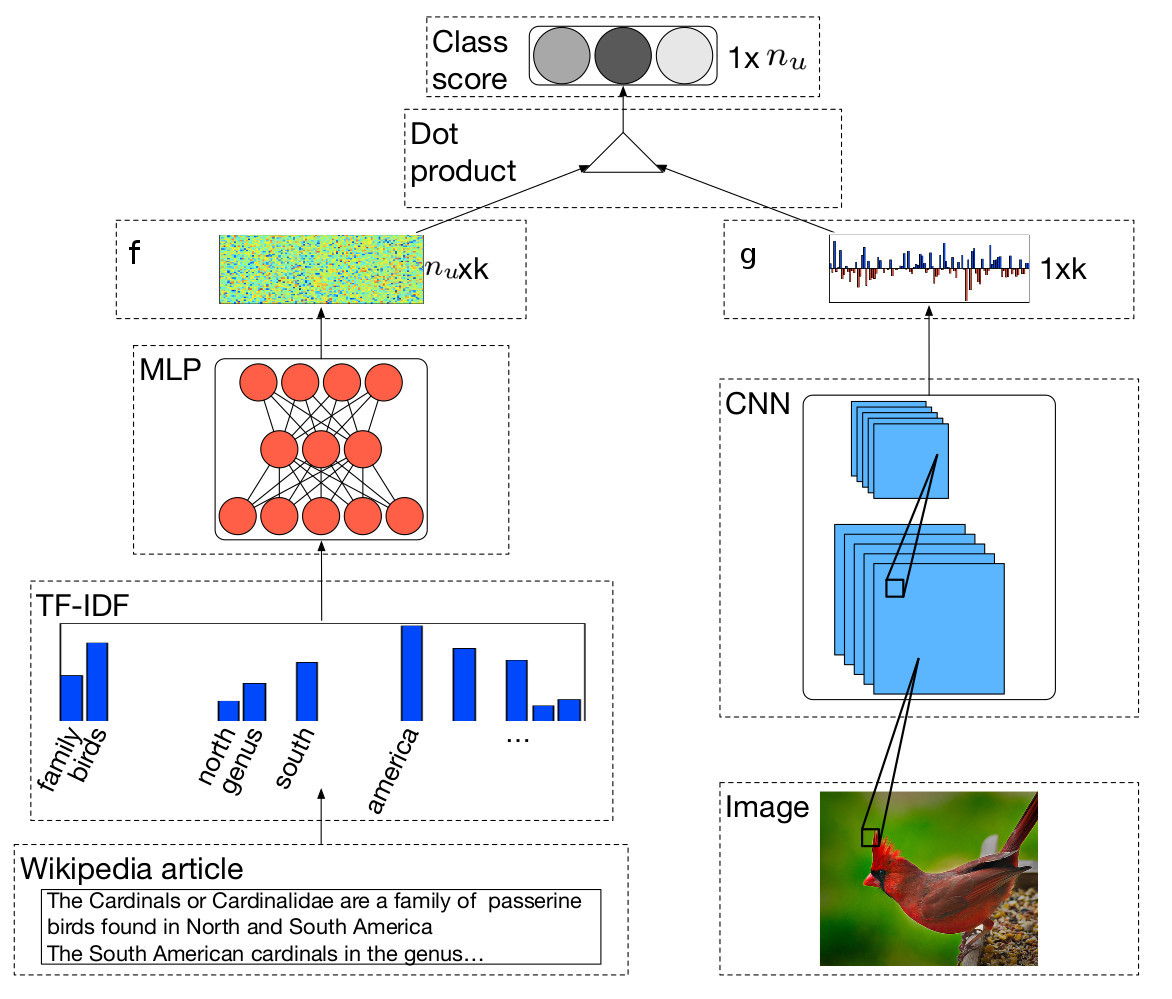
\includegraphics[width=7cm]{images/ba.jpg}
\end{center}
\caption{
 شبکه مورد استفاده برای یادگیری توام نگاشت تصاویر و توصیف‌ها که یک شبکه عصبی عمیق با دو ورودی است. ورودی اول از نوع تصویر است و ابتدا با یک شبکه کانولوشنال سپس با چند لایه چگال به فضایی $k-$بعدی می‌رود. ورودی دوم که یک مقاله از ویکی‌پدیای انلگیسی است پس از تبدیل به نماش برداری به صورت \lr{tf-idf} با چندلایه با اتصالات چگال پردازش شده و به فضایی $k-$بعدی می‌رود. در نهایت امتیاز تعلق تصویر به دسته‌ی متن با ضرب داخلی این دو نگاشت تعیین می‌شود \cite{ba2015}.
}
\end{figure}

در  \cite{ba2015} از شبکه‌های عصبی عمیق برای یادگیری توام نگاشت‌های $\phi$ و $\theta$ استفاده شده است. نمای کلی شبکه مورد استفاده در این روش در تصویر
\ref{fig:deep}
نشان داده شده است. توصیف‌های متنی و ويژگی‌های بصری دو ورودی جداگانه به چنین شبکه‌ای هستند که ابتدا به صورت جداگانه با یک یا چند لایه‌ی با اتصالات کامل به یک فضای مشترک نگاشته شده و سپس بر اساس شباهت نمایش آن‌ها در این فضای میانی دسته‌بندی می‌شوند. تفاوت این روش با سایر روش‌هایی که مرور شد یادگیری توامان نگاشت‌های  $\phi$ و $\theta$ است که با استفاده از شبکه‌های عصبی ممکن شده است. معیار یادگیری این دو نگاشت تنها خطای دسته‌بندی نهایی است.
این روش را می‌توان به صورت ساخت دسته‌بند از روی توصیفات نیز تعبیر کرد؛ با این تفاوت که در این حالت یک تبدیل نیز روی فضای تصاویر اعمال شده و سپس دسته‌بند خطی یادگرفته شده از متون در این فضا به نگاشت تصاویر اعمال می‌شود. در این حالت دسته‌بند خطی $w^y$ یک تابع غیر خطی از توصیف کلاس $y$ است: $w^y = f(c^y)$ که $f$ شبکه عصبی مخصوص متن است (نیمه‌ی چپ تصویر \ref{fig:deep}.) استخراج ویژگی غیر خطی از تصاویر نیز با یک شبکه عصبی که تابع آن را $g$ می‌نامیم، انجام شده است(نیمه‌ی راست تصویر \ref{fig:deep}.) در نهایت دسته‌بندی با تابع زیر انجام می‌شود:
\begin{equation} \label{eq:ba_classifier}
y^* = \argmax_y{w^{yT} g(x)}.
\end{equation}
این روش فراتر از دسته‌بند خطی به حالت فوق نیز با معرفی دسته‌بند کانولوشنال توسعه پیدا می‌کند. در شبکه‌های عصبی کانولوشنال، اطلاعات مکانی در  لایه‌های با اتصال چگال از بین می‌رود. هم‌چنین تعداد وزن‌ها در این لایه‌ها بسیار بیشتر از لایه‌های کانولوشنال زیرین است. در نتیجه بنظر می‌رسد استفاده مستقیم از خروجی لایه‌ی کانولوشنال و اضافه کردن یک لایه کانولوشنال دیگر یادگیری فیلتر بر اساس متن می‌تواند راه‌حل مناسب‌تری از یادگیرفتن یک یا چند لایه‌ی چگال باشد.

فرض کنید $b$ خروجی یک لایه‌ی کانولوشنال با $M$ نقشه از ویژگی‌های تصویر باشد: $b \in \mathbb{R}^{M\times l \times h}$ که $h$ و $l$ ارتفاع و عرض نقشه ویژگی‌ها هستند. دسته‌بند روی $b$ به صورت یک لایه‌ی کانولشنال فورمول‌بندی می‌شود. ابتدا یک کاهش ابعاد غیر خطی روی هر یک از نقشه‌های ویژگی صورت می‌گیرد که آن را با $g'$ نشان می‌دهیم:
$g': \mathbb{R}^{M\times l\times h} \mapsto \mathbb{R}^{K'\times l\times h}$
که
$K' << M$.
در ادامه از نماد  $a'$ برای نقشه ویژگی کاهش بعد یافته استفاه می‌کنیم
$a' = g'(a)$.
از یک توصیف مثل $c^y$ یک  فیلتر کانولوشن $w^y = f'(c^y)$ ایجاد می‌شود که اگر اندازه فیلتر را با $m$ نشان دهیم: $w'_c \in \mathbb{R}^{K' \times m \times m}$. همانند حالت قبل، $f'$ با یک شبکه عصبی چند لایه مشخص می‌شود. در نهایت دسته‌بند کانولوشنال به صورت زیر تعریف می‌شود:
\begin{align}
\label{eq:conv}
\text{score}(x,y)=o\bigg(\sum_{i=1}^{K'}w^{y'}_{i}\  \check{*} \  a'_i\bigg),
\end{align}
 $\text{score}(x,y)$
  امتیاز تعلق $x$ به دسته‌ی $y$ است؛ $o(\cdot)$ یک تابع ادغام\LTRfootnote{pooling} به صورت $o:\mathbb{R}^{l\times h} \mapsto \mathbb{R}$  و $\check{*}$ نشان‌گر عمل کانولوشن است. در این حالت فیلترهای یادگرفته شده به علت این که به محل تصویر وابسته هستند می‌توانند با دقت بهتری تطابق توصیف‌های متنی و تصویر را نشان دهند.

  در نهایت در این پژوهش استفاده همزمان از دسته‌بندهای خطی و کانولوشنال پیشنهاد می‌شود که در با استفاده از آزمایشات عملی نشان داده شده عمل‌کرد بهتری خواهد داشت. برای استفاده همزمان از این دو دسته‌بند امتیاز تطابق از جمع این دو بدست می‌آید:
\begin{align}
\text{score}(x,y)=w^{yT}g(x) + o\bigg(\sum_{i=1}^{K'}w^{y'}_{i}\  \check{*} \  g'(a)_i\bigg).
\end{align}
در این حالت پارامترهای مربوط به $g, g', f , f'$ به صورت همزمان یادگرفته می‌شوند.
یادگیری در شبکه بر اساس خطای تنها خروجی که نشان می‌دهد آیا این متن و توصیف هم‌دسته هستند یا نه صورت می‌گیرد. در این پژوهش دو تابع هزینه برای خطا در نظر گرفته شده ۱) آنتروپی تقاطعی
\LTRfootnote{Cross Entropy}
۲) تابع هزینه لولا\LTRfootnote{hinge loss}. بررسی عمل‌کرد این دو نوع تابع هزینه نشان می‌دهد که بر اساس معیار ارزیابی نهایی هر کدام می‌توان عمل‌کرد بهتری نسبت به دیگری داشته باشد. اگر معیار ارزیابی دقت دسته‌بندی در $k$ انتخاب اول\LTRfootnote{top-k accuracy} باشد تابع هزینه لولا بهتر عمل می‌کند و اگر معیار مساحت زیر نمودار صحت و بازیابی\LTRfootnote{Precision Recall Area Under the Curve} باشد، آنتروپی متقاطع عمل‌کرد بهتری دارد.

\subsection{نگاشت به فضای دسته‌های دیده شده}
با توجه به این که یادگیری تابع تعیین شباهت هر نمونه با دسته‌های آموزش تنها به نمونه‌های آموزش نیاز دارد می‌تواند به طور کامل در زمان آموزش انجام شود. بر این اساس اگر دسته‌های دیده نشده به خوبی بر اساس شباهتشان با دسته‌های دیده شده قابل توصیف باشند، می‌توان یک معیار مطابقت میان آن‌ها و نمونه‌های آزمون بدست آورد. (مثلا بر اساس ضرب داخلی یا فاصله اقدلیدسی در این فضا) در زمینه‌ی یادگیری بدون برد چند روش بر این اساس ارائه شده است. بعضی از این روش‌ها توصیف دسته‌های آزمون بر اساس دسته‌های آموزش را به عنوان ورودی دریافت می‌کنند و برخی دیگر توانایی بدست آوردن این نمایش را بر اساس توصیف‌های جانبی دارند. 


 



%------chapter 3: works
\chapter{روش پیشنهادی} \label{chap:proposed}
در این فصل به بیان روش‌های پیشنهادی در این پژوهش برای مسئله یادگیری صفرضرب می‌پردازیم. روش‌های مطرح شده در این فصل از دو رویکرد متفاوت برای حل مسئله یادگیری صفرضرب استفاده می‌کنند. یک رویکرد یافتن نگاشت از فضای تصاویر به فضای توصیف دسته‌هاست که این نگاشت با استفاده از شبکه‌های ژرف مدل شده است. رویکرد دوم انجام یک خوشه‌بندی در فضای ویژگی‌های ژرف استخراج شده از تصاویر که نمونه‌های آزمون را در خوشه‌هایی تقسیم می‌کند و با یادگرفتن نگاشتی از فضای توصیف دسته‌ها به فضای ویژگی‌های ژرف تصاویر هر خوشه بر یکی از دسته‌های دیده نشده انطباق داده می‌شود.

در ابتدای این بخش به مسئله استخراج ویژگی از تصاویر با استفاده از شبکه‌های ژرف می‌پردازیم، فضای تشکیل شده از ویژگی‌های تصاویر هنگام استفاده از این شبکه‌ها، دارای خاصیت جدایی پذیری دسته‌های مختلف از هم و تشکیل خوشه‌هایی از نمونه‌های هر دسته است؛ فرض وجود چنین خاصیت‌هایی در فضای ویژگی‌های تصاویر، اساس روش‌های ارائه شده در این فصل است.
در بخش \ref{nn} یک شبکه‌ی عصبی چندوظیفه‌ای برای پیش‌بینی ویژگی از تصاویر معرفی می‌کنیم که با در نظر گرفتن نمونه‌های آزمون در زمان آموزش می‌تواند مشکل جابجایی دامنه را کاهش دهد.
در بخش
\ref{clustering_method}
 یک تابع مطابقت نوین برای مسئله دسته‌بندی صفرضرب معرفی می‌کنیم که استفاده از اطلاعات غیرنظارتی موجود در ساختار نمونه‌های دسته‌های دیده نشده را ممکن می‌سازد. این تابع مطابقت از یک خوشه‌بندی روی نمونه‌های آزمون بهره می‌برد که با توجه به استخراج ویژگی‌ها با استفاده از شبکه‌های عصبی ژرف و جداسازی مناسب در فضای این ویژگی‌ها، از دقت مناسبی برخوردار است. این تابع مطابقت به نمونه‌هایی که در یک خوشه قرار دارند برچسب یکسانی نسبت می‌دهد. با توجه به استفاده از خوشه‌بندی در این تابع مطابقت، یک روش خوشه‌بندی نیمه‌نظارتی که منطبق بر فرضیات مسئله یادگیری صفرضرب است ارائه می‌گردد و سپس یک روش دسته‌بندی با استفاده از تابع مطابقت و خوشه‌بندی ارائه شده و یادگیری نگاشتی خطی از توصیف دسته‌ها به فضای تصاویر، تدوین می‌گردد. هرچند که عملکرد این روش ارائه شده برتر از روش‌های پیشگام موجود است ولی محدودیت‌هایی نیز دارد که ناشی از جدا بودن مرحله خوشه‌بندی و نگاشت به فضای مشترک است؛ برای رفع این محدودیت‌ها روش دیگری معرفی می‌شود که خوشه‌بندی و یادگیری نگاشت در آن به صورت توام انجام می‌شود. این یادگیری توام باعث بهبود دقت دسته‌بندی نسبت به روش پیشنهادی قبلی می‌شود.

نمادگذاری مورد استفاده در این فصل سازگار با نمادگذاری معرفی شده در بخش ۲ است که در جدول \ref{tab:notation} برای مراجعه سریع خلاصه شده است.
\begin{center}
\begin{table}[ht]
\centering
\caption{معرفی نمادهای مورد استفاده}
\vspace{2mm}
\label{tab:notation}
\begin{tabular}{|c|r|}
\hline
 نماد &  شرح \\
\hline
  $\mathcal{S}(\mathcal{U})$ & \rl{مجموعه دسته‌های دیده‌شده (دیده‌نشده) }     \\\hline
  $n_s (n_u) $ & \rl{تعداد دسته‌های دیده‌شده (دیده‌نشده) }   \\\hline
  $N_s (N_u) $ & \rl{تعداد نمونه‌های آموزش (آزمون) }   \\\hline
  $X_s (X_u) $ & \rl{ماتریس نمونه‌های آموزش (آزمون) }   \\\hline
  $Y_s (Y_u) $ & \rl{برچسب‌های نمونه‌های آموزش (آزمون) }   \\\hline
  $C_s (C_u) $ & \rl{ماتریس توصیف‌های دسته‌های دیده‌شده (دیده‌نشده) }   \\\hline
  $\mathbf{x_i}  \in \mathbb{R}^d$ & \rl{ بردار ویژگی‌های تصویر $-i$م}   \\\hline
 $ \mathbf{c_y}  \in \mathbb{R}^a$ & \rl{بردار توصیف دسته‌ی $y$}   \\\hline
\hline
 $X_{(i)}$ & \rl{سطر $-i$م ماتریس $X$} \\ \hline
 $\normf{X}$ & \rl{نرم فروبنیوس ماتریس $X$} \\ \hline
 $diag(\mathbf{x})$ & \rl{یک ماتریس قطری که بردار $\mathbf{x}$ روی قطر اصلی آن قرار داده شده} \\ \hline
 $\mathbf{1}$ & \rl{یک بردار که تمام عناصر آن برابر یک است} \\ \hline
 $\mathbf{1}_k$ & \rl{یک بردار که درایه‌ی $-k$م آن یک و سایر عناصرش صفر است } \\ \hline
\end{tabular}
\end{table}
\end{center}

\section{استخراج ویژگی با شبکه‌های عصبی ژرف}\label{cnns}
عمل‌کرد مناسب روش‌های بینایی ماشین از جمله روش‌هایی دسته‌بندی صفرضرب تصاویر  وابستگی زیادی به نمایش بدست آمده از تصاویر دارد. در سال‌های اخیر استفاده از شبکه‌های عصبی پیچشی ژرف کاراترین روش برای استخراج ویژگی از تصاویر بوده است \cite{Oquab2014}. این روش که در آن نحوه‌ی استخراج ویژگی با استفاده از تعداد زیادی داده‌ی برچسب‌دار
\textit{یاد گرفته می‌شود،}
جایگزین روش‌های قبلی مانند SIFT و HOG شده است که در آن‌ها، نحوه‌ی استخراج ویژگی توسط یک خبره تعیین شده و همواره ثابت است.

معماری شبکه‌های عصبی ژرف پیچشی مبتنی بر خاصیت \gls{stationary} بودن تصاویر است، این خاصیت به این معناست که خواص آماری نواحی مختلف تصاویر با یکدیگر یکسان هستند. در نتیجه‌ی وجود این خاصیت \gls{filter} مورد برای استخراج \gls{localfeat} از تصویر در تمام مکان‌های تصویر یکسان در نظر گرفته می‌شود. چنین نگاشتی با عمل پیچش قابل مدل‌سازی است. فرض کنید که $v$ یک تصویر $M\times N$ باشد و $W$ یک صافی خطی، آن‌گاه یک لایه‌ی پیچشی از یک شبکه عصبی به صورت زیر تعریف می‌شود:
\begin{align}
h_1^{(k)} &= g(W^k \ast v + b^k) \label{eq:conv_layer}\\
(W \ast x)_{m,n} &= \sum_{i=-\infty}^{\infty} \sum_{j=-\infty}^{\infty} W_{i,j} x_{m -i, n-j}.
\end{align}
در این رابطه $h^{(1)}$ مقادیر لایه نهان اول شبکه را نشان می‌دهد و $b$ جمله‌‌ی بایاس است، $g$ یک  \gls{ActivationFunction} مانند $tanh$ است. در این حالت فیلتر $W$ که عموما اندازه بسیار کمتری نسبت به تصویر دارد (برای مثال $3 \times 3$ یا
$ 7 \times 7$)
بر تصویر اعمال می‌شود تا ویژگی‌هایی از تصویر استخراج کند. این مدل‌سازی مشابه روش‌های قدیمی‌تری است که مثلا برای تشخیص لبه و گوشه استفاده می‌شوند \cite{harris1988}. مهم‌ترین تفاوت شبکه‌های عصبی و آن روش‌ها در این است که مقادیر فیلتر $W$ یادگرفته می‌شوند و از پیش توسط خبره معین نشده‌اند. همچنین در این شبکه‌ها در هر لایه عموما از چندین صافی استفاده می‌شود و چند  تعداد کم پارامترهای فیلتر و استقلال آن از اندازه تصویر ورودی، باعث شده تعداد پارامتر‌های موجود در یک لایه‌ی پیچشی بسیار کمتر از یک \gls{fully-connected-layer} باشد و در نتیجه امکان افزایش عمق شبکه بیشتر باشد. در نتیجه در شبکه‌های عصبی معمولا از چندین لایه‌ی پیچشی استفاده می‌شود.
\begin{figure}[!t]
\centering
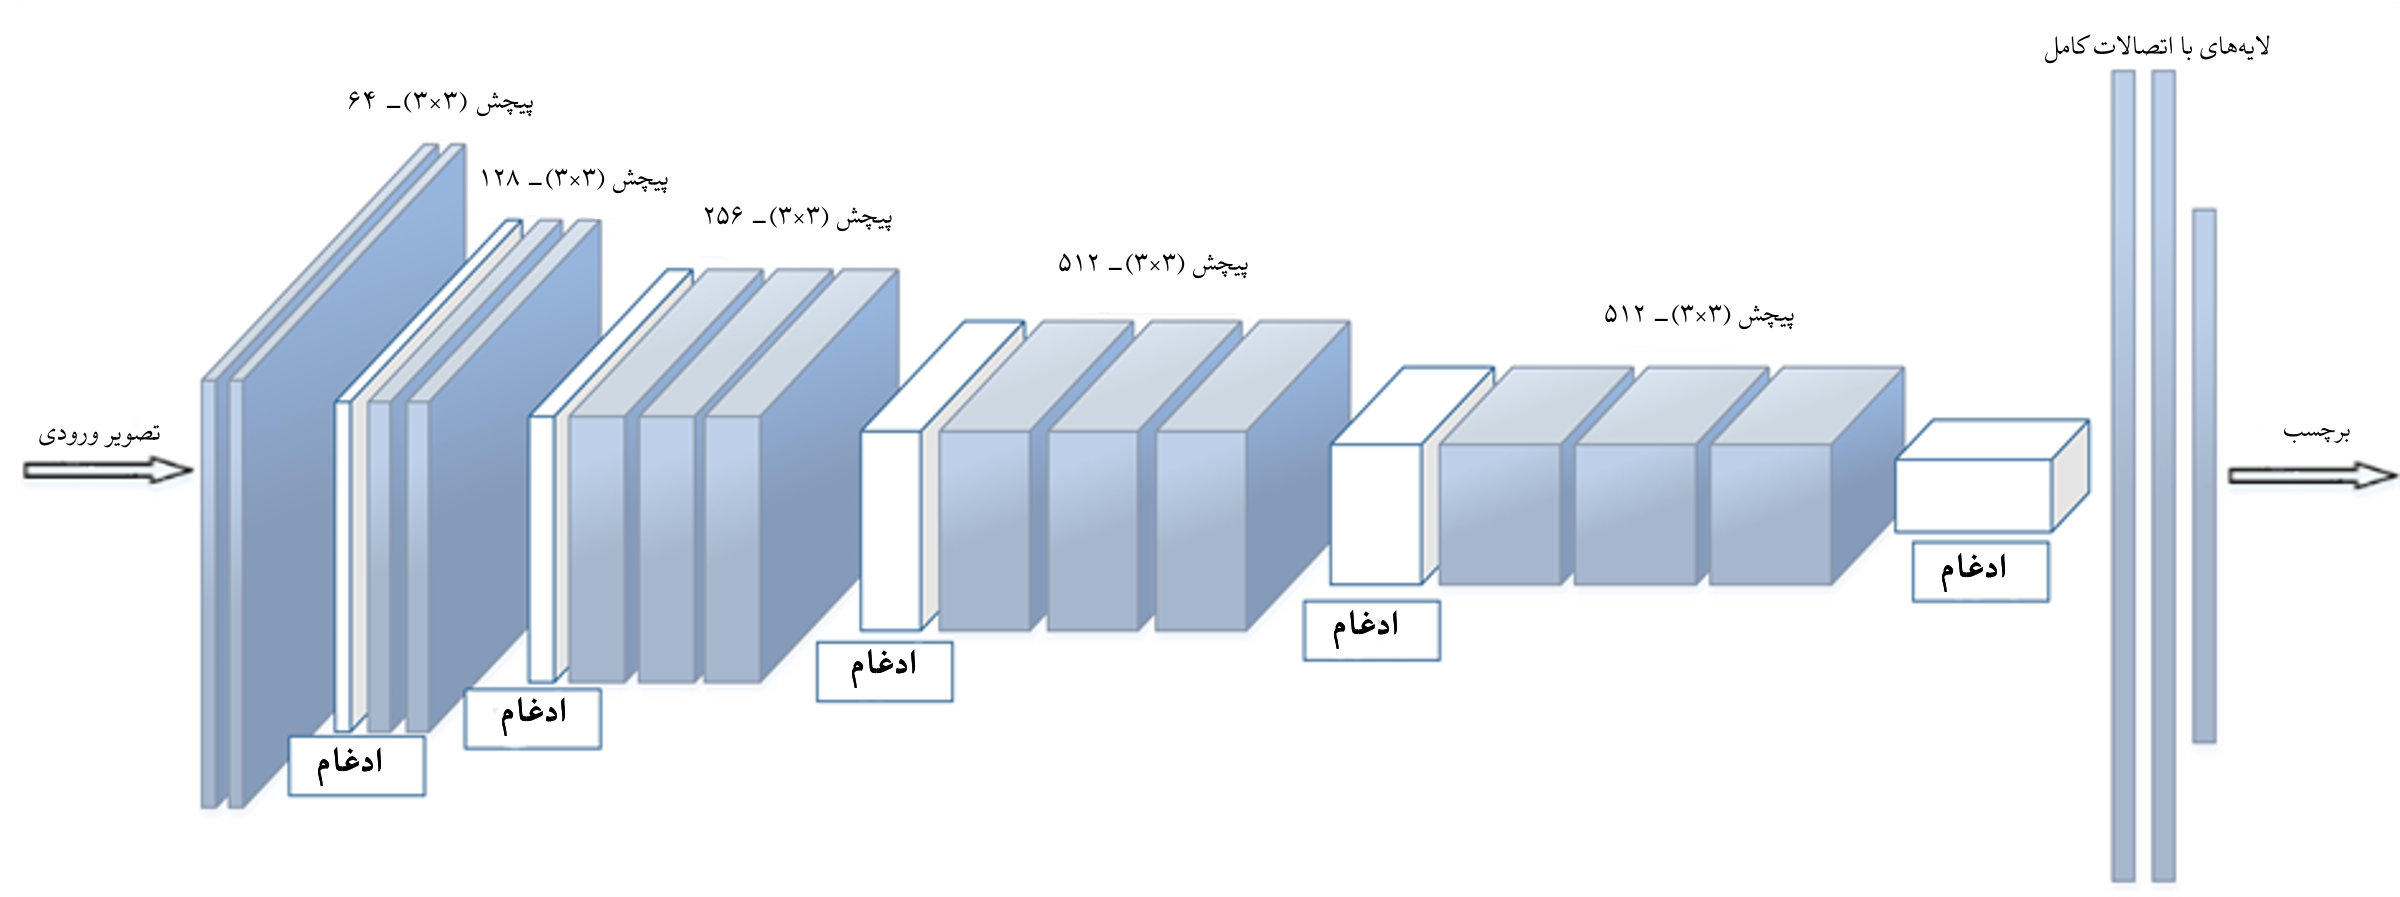
\includegraphics[width=1.1\linewidth]{images/vgg}
\caption[ساختار شبکه استخراج ویژگی]{
ساختار شبکه vgg که در آن لایه‌های سفید مراحل ادغام که اینجا انتخاب بیشینه در پنجره‌های $2 \times 2$ است را نشان می‌دهند.
لایه‌های پیچشی با مکعب‌های آبی مشخص شده‌اند که عرض آن‌ها متناسب با تعداد کانال‌های موجود در آن لایه است \cite{el2016face}.
}
\label{fig:vgg}
\end{figure}
معماری مورد استفاده در روش‌های این فصل برای استخراج ویژگی، مبتنی بر معماری ۱۹ لایه شبکه \lr{vgg} \cite{vgg} است (شکل \ref{fig:vgg}). در این شبکه از ۱۶ لایه‌ی پیچشی استفاده شده است. ساختار هر لایه به این صورت است که تعدادی کانال از ویژگی‌ها (در لایه‌ی اول  خود تصویر) به عنوان ورودی وارد لایه می‌شوند و با استفاده از تعدادی صافی با اندازه $3 \times 3$ به ویژگی‌های خروجی تبدیل می‌شوند. تعداد کانال‌های ورودی در لایه‌ی اول سه کانال رنگی \lr{RGB} است و در لایه‌های بعدی تعداد صافی‌ها به گونه‌ای تعیین شده که تعداد کانال‌های ویژگی‌ها برابر: ۶۴ در لایه‌ی اول و دوم، ۱۲۸ در لایه‌ سوم و چهارم، ۲۵۶ در لایه پنجم تا هشتم و ۵۱۲ در لایه نهم تا شانزدهم است. \gls{ActivationFunction} مورد استفاده در لایه‌های پیچشی تابع \gls{ReLU} است که ضابطه آن به این صورت است:
\begin{equation}
ReLU(\mathbf{x}) = max(\mathbf{0,x}).
\end{equation}
 برای کاهش اندازه ماتریس ویژگی‌ها، میان برخی لایه‌های پیچشی از یک تابع \gls{pooling} استفاده می‌شود. تابع \gls{pooling} مورد استفاده در این شبکه تابع \gls{pooling} بیشینه است یعنی در ماتریس ویژگی‌ حاصل یک پنجره‌ی $2 \times 2$ حرکت داده می‌شود و تنها بزرگترین مقدار میان چهار مقداری پنجره بر آن‌ها منطبق شده به خروجی منتقل می‌شود. بعد از ۱۶ لایه پیچشی سه \gls{fully-connected-layer} وجود دارد. ما برای استخراج ویژگی از خروجی لایه‌ی هدفهم یعنی نخستین  \gls{fully-connected-layer} استفاده می‌کنیم و دو لایه‌ی نهایی کنار گذاشته می‌شوند. ورودی این لایه به این صورت به دست می‌آید که تمام ماتریس‌های ویژگی لایه‌ی شانزدهم به صورت بردارهای یک بعدی در آمده و در کنار هم قرار می‌گیرند، سپس به صورت یک برادر $-25088$ بعدی وارد لایه‌ی هفدهم شده و در این لایه با استفاده از یک نگاشت خطی و \gls{ActivationFunction}   \gls{ReLU} به بردارهای ویژگی $-4096$بعدی تبدیل می‌شود. در شبکه اصلی این خروجی این لایه به یک لایه‌ی مشابه خود و سپس در نهایت با یک لایه \gls{fully-connected-layer} که خروجی آن به اندازه تعداد دسته‌هاست با  \gls{ActivationFunction}
 \lr{softmax}
 به پیش‌بینی برچسب تبدیل می‌شود.

\section{یک شبکه‌عصبی چندوظیفه‌ای}\label{nn}
\begin{figure}[!t]
\centering
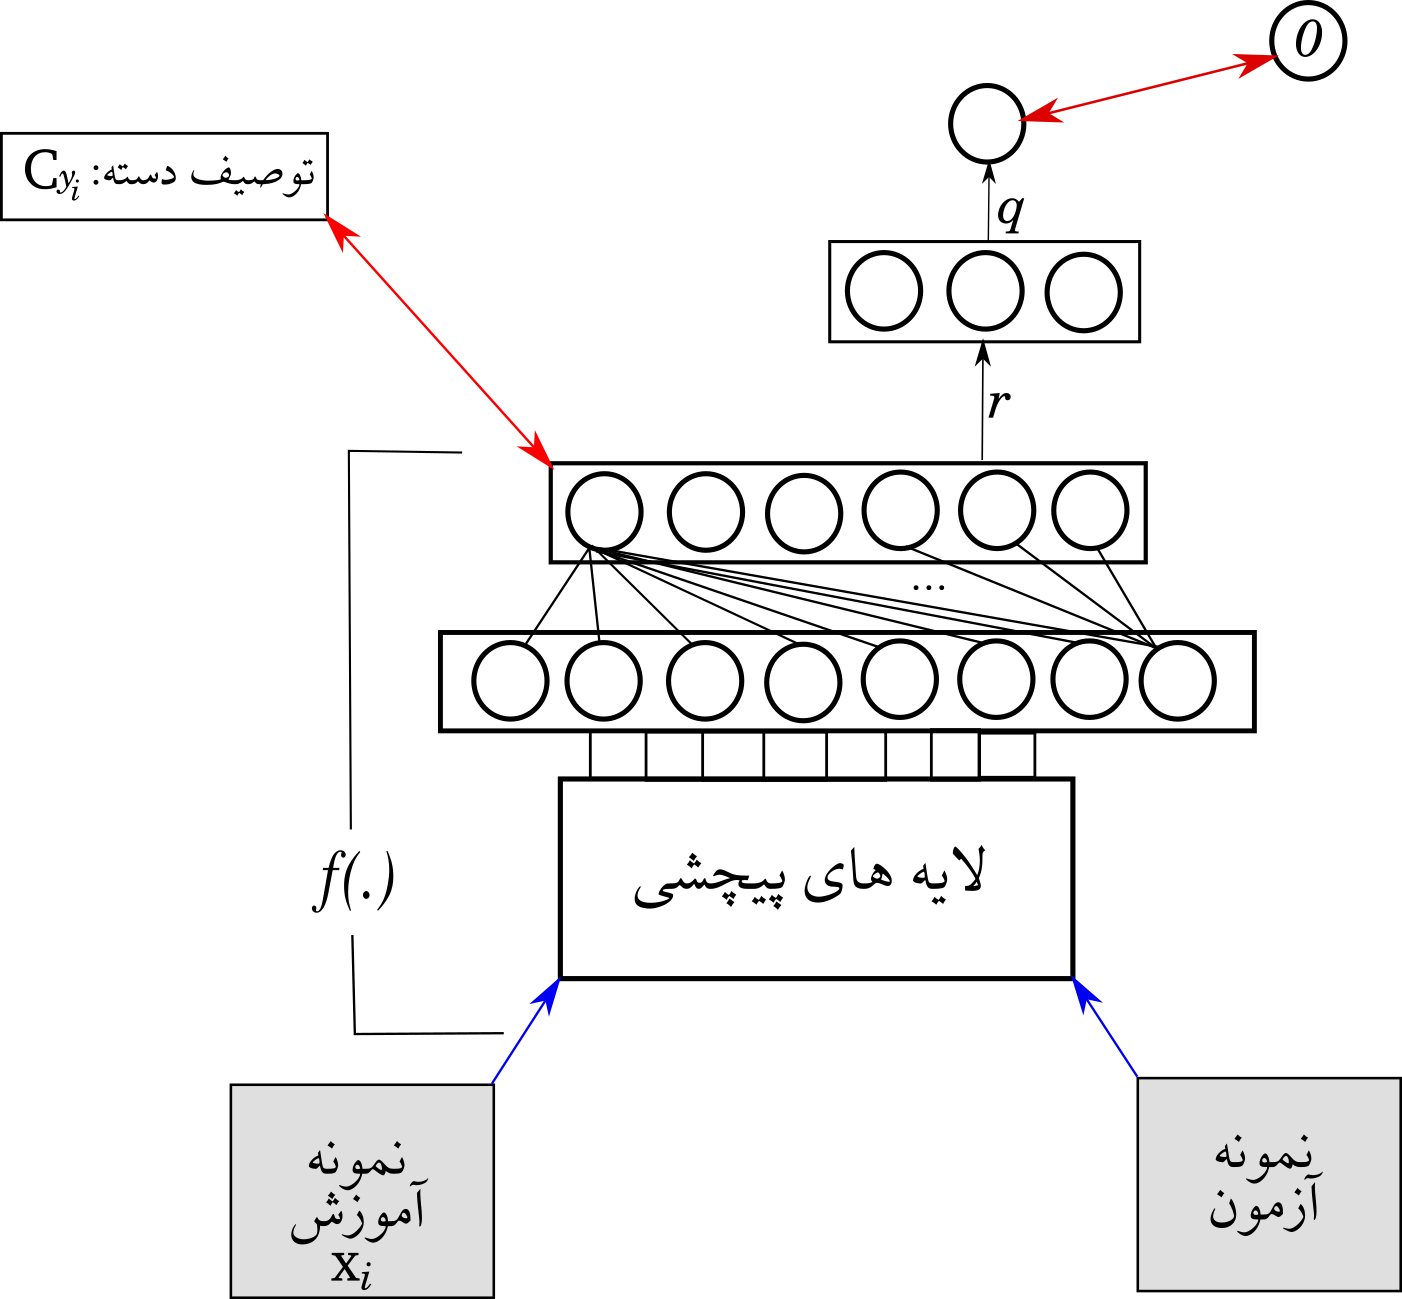
\includegraphics[width=0.85\linewidth]{images/net}
\caption[شبکه‌ی چندوظیفه‌ای پیشنهادی]{
ساختار شبکه چند وظیفه‌ای پیشنهادی. فلش‌های آبی رنگ ورودی‌های شبکه را نشان می‌دهند و فلش‌های قرمز رنگ مقایسه خروجی شبکه با خروجی مورد انتظار را. خطوط سیاه‌رنگ اتصالات شبکه‌ را نشان می‌دهند. زیر شبکه‌ی برگرفته شده از شبکه vgg و یک لایه‌ی با اتصالات چگال اضافه شده بین دو دو ورودی مشترک هستند. لایه‌های $r$ و $q$ مخصوص نمونه‌های آزمون هستند. خروجی لایه‌ی $q$ همواره با مقدار صفر مقایسه می‌شود.
}
\label{fig:nn2}
\end{figure}

یادگیری نگاشت‌ها با استفاده از داده‌های دسته‌های دیده‌شده، همان‌طور که در بخش \ref{lr:semi} اشاره شد، دچار مشکل جابجایی دامنه است و  روی داده‌های دسته‌های دیده‌نشده به خوبی قابل تعمیم نیست. یک راه حل برای مقابله با این مشکل این است که در حین یادگیری نگاشت اجبار شود که حاصل نگاشت یک نمونه‌ی آزمون به نوعی نزدیک به نگاشت توصیف دسته‌های آزمون باشد. همان ‌طور که در بخش
\ref{lr:semi}
بیان شد، چنین راه‌حلی در
\cite{Kodirov2015}
استفاده شده است. معیار نزدیکی نگاشت‌ها در آن روش یک امتیاز پیشین از شباهت هر نمونه‌ی آزمون با دسته‌های دیده نشده است که  توسط یک روش دیگر استخراج شده می‌شود. یعنی ابتدا یک روش دسته‌بندی
احتمالی  که در آن پژوهش روش \lr{IAP} \cite{lampert09} برای این کار انتخاب شده بود، به صورت مستقل روی مجموعه دادگان اجرا شده و احتمال‌هایی که برای انتساب هر نمونه به دسته‌های آزمون از آن روش بدست می‌آید بعنوان وزن‌های شباهت در نظر گرفته می‌شود و فاصله هر توصیف پیش‌بینی شده برای هر نمونه با توصیف دسته‌های آزمون متناسب با این وزن‌های شباهت جریمه می‌شود.
 ما در این بخش یک روش مبتنی بر شبکه‌های عصبی ژرف معرفی می‌کنیم که در آن نگاشتی غیرخطی و چندلایه از تصاویر به بردارهای صفت یادگرفته می‌شود. معیار یادگیری این نگاشت، پیش‌بینی صحیح صفت برای نمونه‌های آموزش (که بردار صفت صحیح برای آن‌ها مشخص است) و هم‌چنین نزدیک بودن حاصل نگاشت هر نمونه‌ی آزمون به توصیف یکی از دسته‌های دیده نشده است. برای مدل کردن این نگاشت، از یک شبکه‌ی عصبی استفاده شده است. اگر نگاشت مدل شده با شبکه عصبی را با $f$ نشان دهیم، تابع هزینه‌ی مورد استفاده برای آموزش شبکه به صورت زیر تعریف می‌شود:
\begin{equation}
\label{eq:nn_loss}
\min_{f}
\frac{1}{N_s} \sum_{n=1}^{N_s} loss(f(\mathbf{x_i), c_{y_i}}) +
\frac{\beta}{N_u} \sum_{i=N_s}^{N_s+N_u} \Big ( \min_{j=n_s,\ldots,n_s + n_u} \normtwo{f(\mathbf{x_i) - c_j}} \Big ),
\end{equation}
که $\beta$ یک فراپارامتر است.
جمله‌ی اول، جمله‌ی مربوط به خطایی پیش‌بینی صفت‌هاست تفاوت میان صفات پیش‌بینی شده توسط شبکه و صفات صحیح را برای نمونه‌های آموزش جریمه می‌کند.
 جمله‌ی دوم برای رفع مشکل جابجایی دامنه طراحی شده است و تحمیل می‌کند که حاصل نگاشت یک نمونه‌ی آزمون حتما نزدیک توصیف یکی از دسته‌های دیده‌نشده باشد، این دسته‌ی دیده نشده، دسته‌ای در نظر گرفته شده است که توصیف آن با نگاشت کمترین فاصله را دارد. این قسمت از رابطه فوق را می‌توان به صورت شهودی این گونه توضیح داد که در غیاب جمله‌ی دوم برای هر نمونه یک بردار توصیف پیش‌بینی می‌شد و سپس نزدیک‌ترین بردار توصیف از میان توصیف دسته‌های آزمون به عنوان توصیف صحیح در نظر گرفته شده و برچسب بر اساس آن پیش‌بینی می‌شد. حال جمله‌ی دوم رابطه \eqref{eq:nn_loss} جریمه‌ای به میزان فاصله‌ی توصیف پیش‌بینی شده برای هر نمونه با بردار توصیف همان دسته‌ای که به آن نزدیک‌تر است، در نظر می‌گیرد. حال اگر این فرض صحیح باشد که
 حاصل نگاشت در اکثر موارد به توصیف صحیح نزدیکتر است، یا به عبارتی این که در اکثر مواقع استفاده از دسته‌بند نزدیکترین همسایه روی نگاشتی که تنها با جمله‌ی اول آموزش دیده، دقتی بیش از ۵۰٪ دارد، وجود چنین جمله‌ای باعث می‌شود که مواردی که قبلا درست تشخیص داده می‌شدند حالا با دقت بیشتر (فاصله کمتر از بردار توصیف دسته‌ی مورد نظر) باز هم درست پیش‌بینی شوند. با توجه به افزایش دقت نگاشت روی این نمونه‌ها، انتظار می‌رود برای برخی نمونه‌هایی که در حالت قبل پیش‌بینی نادرست به آن‌ها تعلق می‌گرفت نیز با این نگاشت بهبود یافته، پیش‌بینی صحیح برای آن‌ها صورت بگیرد.

 تابع $loss(\cdot, \cdot)$ در معادله \eqref{eq:nn_loss} در مجموعه دادگانی که صفات دودویی هستند تابع \gls{crossentropy} متقاطع در نظر گرفته شده است یعنی:
 \begin{equation}
 loss(y,z) = z \log(1-y) + (1-z) \log(y).
 \end{equation}
 برای مجموعه دادگانی که مقادیر بردارهای توصیف در آن‌ها مقادیر دلخواه حقیقی است تابع خطای مربع اختلاف در نظر گرفته شده است:
 \begin{equation}
 loss(y,z) = \normtwo{y-z}.
 \end{equation}
 \subsection{بهینه‌سازی }\label{opt_nn}

 تابع کمینه به کاربرده شده در جمله‌دوم معادله
\eqref{eq:nn_loss}
در برخی نقاط مشتق‌پذیر نیست، اما با توجه به اینکه اندازه‌ی این نقاط صفر است تابع تقریبا همه‌جا مشتق‌پذیر است و آموزش شبکه با استفاده از \gls{backprop}
 مقدار گرادیان ممکن خواهد بود. به صورت دقیق‌تر، بهینه‌سازی رابطه \eqref{eq:nn_loss} عملیات محاسبه‌ی مقدار کمینه را داخل شبکه تعبیه می‌کنیم (شکل \ref{fig:nn2})؛ به این صورت که لایه‌های جدید $q$ و$r$ برای نمونه‌های دیده نشده اضافه می‌شود که:
\begin{align}
\label{eq:min_layer}
(q(\mathbf{v}))_j &=  \normtwo{f(\mathbf{v) - c_j}}, \\
r(\mathbf{z}) &= \min_{j=1\ldots n_u} (\mathbf{z})_j.
\end{align}
در رابطه \eqref{eq:min_layer}، لایه‌ی $q$ یک بردار توصیف پیش‌بینی شده را به در ورودی دریافت کرده است و خروجی آن برداری است که تعداد ابعادش برابر تعداد دسته‌های دیده‌نشده است و مقدار هر بعد آن برابر فاصله‌ی بردار $v$ با بردار توصیف (امضای) یک دسته‌ی دیده‌نشده. سپس خروجی این لایه به لایه‌ی $r$ وارد می‌شود و در این لایه کوچکترین مقدار این بردار انتخاب می‌شود. نتیجتاً ترکیب این دولایه کمینه‌ی فاصله‌ی $v$ با امضاهای دسته‌های دیده‌نشده را تولید خواهد کرد که برابر جمله‌ی دوم در رابطه \eqref{eq:nn_loss} خواهد بود.

در هنگام آموزش با پس‌انتشار، مشق تابع هزینه‌ی $l$ نسبت به هر ورودی مثل $z$ در لایه‌ی $r$ با ضابطه‌ی زیر محاسبه می‌شود:
\begin{equation}
\label{eq:grad_min}
\frac{\partial l}{\partial z} = \sum_j \mathds{1}[(z)_j=\min(z)] \cdot \frac{\partial l}{(z)_j}.
\end{equation}

پس از آموزش شبکه، در فاز آزمون لایه‌های $q$ و $r$ حذف شده و بردار توصیف برای تصاویر آزمون با استفاده از شبکه پیش‌بینی می‌شود، در نهایت دسته‌بندی با استفاده از دسته‌بند نزدیک‌ترین همسایه روی نمونه‌های آزمون انجام خواهد شد. برای اندازه‌گیری میزان شباهت بردارهای صفات در این دسته‌بند از فاصله منهتنی استفاده کرده‌ایم:
\begin{equation}
y^{\star}_n = \mathbf{1}_{\argmin_{j} \norm{f(\mathbf{x_n - c_j})}_1} .
\end{equation}
مراحل آموزش شبکه در الگوریتم \ref{alg:nn} آورده شده است.
\شروع{program}[t!]
	\begin{enumerate}[label={\arabic*},itemsep=.1em, parsep=.1em]
\فقره {\bf ورودی:} تصاویر و توصیف‌های آموزش و آزمون و برچسب‌های نمونه‌های آموزش.
\فقره {\bf خروجی:} برچسب‌های پیش‌بینی شده برای نمونه‌های آزمون.
\فقره پیش آموزش شبکه تنها با نمونه‌های آموزش و مقایسه خروجی با توصیف صحیح.
\فقره آموزش کامل شبکه با داده‌های آموزش و آزمون.
\فقره حذف لایه‌های $r$ و $q$.
\فقره خروجی شبکه را به ازای $X_u$ در $P_u$ بریز.
\فقره دسته‌بند نزدیک‌ترین همسایه $NN$ را با بردارهای توصیف دسته‌های آزمون بساز
\فقره عناصر $P_u$ را با استفاده از $NN$ دسته‌بندی کن.
\فقره حاصل مرحله قبل را به عنوان پیش‌بینی نهایی برگردان.
\end{enumerate}
\caption{الگوریتم آموزش و آزمون شبکه عصبی پیشنهادی}
\label{alg:nn}
\پایان{program}
\subsection{معماری شبکه}\label{net_architechture}
ما از قسمتی از شبکه‌ی ۱۹ لایه‌ی \lr{vgg} \cite{vgg} که شامل ۱۶ لایه‌ی پیچشی ابتدا و لایه‌‌‌اول با اتصالات چگال به عنوان یک زیر شبکه در ورودی شبکه خود استفاده می‌کنیم. همان‌طور که در بخش
\ref{cnns}
شرح داده شد،
 با این زیر شبکه تصاویر ورودی به بردارهای $-4096$بعدی نگاشته می‌شنود. سپس یک لایه‌ی با اتصالات چگال قرار دارد که این حاصل را به بردارهای توصیف دسته‌ها می‌نگارد. برای نمونه‌های آموزش، خروجی این لایه با بردار توصیف صحیح مقایسه می‌شود. برای نمونه‌های آزمون خروجی این لایه به  لایه‌های  $q$ و$r$ متصل می‌شود و مقدار خروجی $r$ با مقدار مطلوبش که صفر است مقایسه خواهد شد.

\gls{ActivationFunction} در همه‌ی لایه‌ها تابع \gls{ReLU} است؛ با این استثنا که برای مجموعه‌ دادگانی که مقادیر بردار توصف دودویی هستند، در لایه‌ی آخر از تابع سیگموید با ضابطه
\begin{equation}
\sigma(x) = \frac{1}{1 + e^{-x}},
\end{equation}
بعنوان \gls{ActivationFunction} استفاده شده است تا مقادیر در بازه‌ی $[0,1]$ نگاشته شوند.

\subsection{یک مدل پایه برای مقایسه}\label{nn_basic}
برای روشن شدن تاثیر استفاده از اطلاعات بدون نظارت نمونه‌های آزمون در یادگیری بهتر نگاشت، مدل ارائه شده را با یک مدل ساده برای پیش‌بینی صفت مقایسه می‌کنیم. در این مدل ساده تنها  از
\glspl{fully-connected-layer}
بعد از استخراج ویژگی با لایه‌های پیچشی، برای پیش‌بینی صفت استفاده می‌کنیم. ساختار این مدل در تصویر \ref{fig:nn_basic} نمایش داده شده است. در این شبکه از یک یا چند
\gls{fully-connected-layer}
بعد از لایه‌های پیچشی استفاده می‌شود. مشابه حالت قبل \gls{ActivationFunction} برای مجموعه دادگانی که مقادیر توصیف دسته‌هایشان دودویی است تابع سیگموید، و برای مجموعه دادگانی که مقادیر بردارهای توصیف در آن‌ها مقادیر دلخواه حقیقی است تابع \gls{ReLU} استفاده شده است.
ابعاد  \gls{fully-connected-layer} پایانی الزاما برابر تعداد ابعاد بردارهای توصیف است و برای سایر   \gls{fully-connected-layer} نیز همین تعداد ابعاد انتخاب شده است.
مقایسه نتایج دقت دسته‌بندی بین مدل قبلی و این مدل در بخش \ref{exp:nn} نشان‌دهنده‌ی تاثیر مثبت استفاده از اطلاعات بدون نظارت موجود در نمونه‌های آزمون است که باعث بهبود حداقل ۱۰ درصدی دقت دسته‌بندی شده است.
\begin{figure}[!ht]
\centering
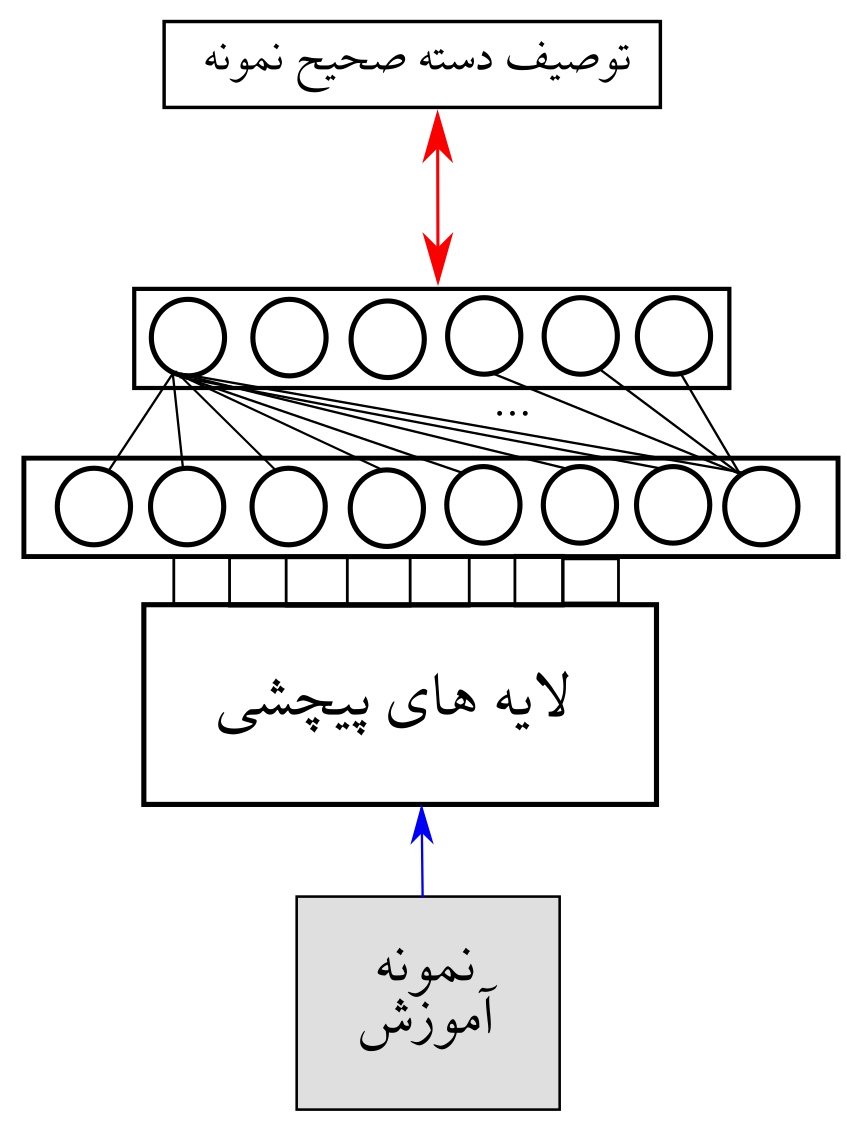
\includegraphics[width=0.4\linewidth]{images/basic_net}
\caption[شبکه‌ی پایه برای پیش‌بینی صفت]{
ساختار شبکه پایه. فلش آبی رنگ ورودی‌های شبکه را نشان می‌دهند و فلش‌های قرمز رنگ مقایسه خروجی شبکه با خروجی مورد انتظار را.}
\label{fig:nn_basic}
\end{figure}
\section{ تابع مطابقت مبتنی بر خوشه‌بندی }\label{compatibility_function}
در اکثر روش‌های پیشین که در فصل \ref{chap:lr} مرور شد، تابع مطابقت میان تصاویر و توصیف‌ها برای اختصاص برچسب به داده‌های آزمون بر اساس فاصله کمینه یا ضرب داخلی بیشینه در یک فضای مشترک محاسبه می‌شد. استثناهای این موضوع، استفاده از روش انتشار برچسب در \cite{Fu2014} و \cite{Kodirov2015} و هم‌چنین پیش‌بینی مستقیم برچسب‌ها در
\cite{li15max}
و
\cite{semi15}
هستند.

\begin{figure}[!t]
\centering
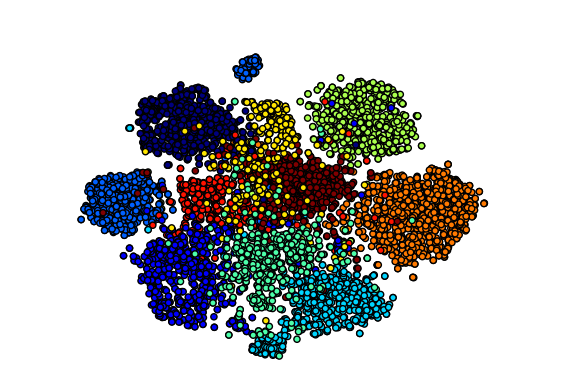
\includegraphics[width=0.85\linewidth]{images/awa_clusters}
\caption[نمایش دسته‌های آزمون مجموعه دادگان AwA ]{
نمایش دوبعدی بوسیله \lr{t-SNE} برای ده دسته‌ی آزمون از مجموعه دادگان AwA با ده رنگ متفاوت نشان داده شده است. درستی فرض قابل خوشه‌بندی در تصویر مشخص است، یعنی ویژگی‌های استخراج شده با استفاده از شبکه‌های ژرف توانایی ایجاد تمایز بالا میان دسته‌ها را دارا هستند.
}
\label{fig:awa_clusters}
\end{figure}

در این بخش ما یک تابع مطابقت جدید بر اساس یک خوشه‌بندی روی داده‌های دسته‌های دیده نشده، تعریف می‌کنیم. اگر فضای نمایش تصاویر دارای این خاصیت باشد که دسته‌های مختلف به صورت خوشه‌های مجزا باشند، استفاده از خوشه‌بندی برای دسته‌بندی برای انتساب برچسب از نظر شهودی توجیه‌پذیر است.
با توجه به نمایش غنی بوجود آمده برای تصاویر توسط شبکه‌های ژرف این فرض در بسیاری از موارد برقرار است. برای نمونه، نمایش \lr{t-SNE} نمونه‌های آزمون مجموعه داده‌های AwA در تصویر
\ref{fig:awa_clusters}
نشان داده شده است و برقراری فرض قابل خوشه‌بندی بودن در آن قابل مشاهده است. این ادعا با استفاده از آزمایش در بخش
\ref{exp:cluster}
اثبات خواهد شد. روش‌های پیشنهادی ما در این فصل بر اساس این ساختار و استفاده از وجود چنین خاصیتی در فضای تصاویر است.
%\section{معرفی یک تابع مطابقت}\label{copatibility_function}

یک راه استفاده از چنین خاصیتی در فضای تصاویر، معرفی یک تابع مطابقت است که علاوه بر شباهت نگاشت‌یافته‌ی نمونه‌ها و توصیف‌ها به سایر نمونه‌های در همسایگی هر نمونه نیز وابسته باشد. بدین منظور ما یک تابع مطابقت جدید پیشنهاد می‌دهیم که در آن برچسب تعلق گرفته به هر نمونه به نمونه‌هایی که با آن‌ها در یک خوشه قرار گرفته است وابسته است. به این منظور ابتدا باید یک خوشه‌بندی روی نمونه‌ها انجام شود سپس با استفاده از یک معیار (که یک نمونه از آن را در بخش \ref{simple_method} معرفی می‌کنیم) میزان شباهت خوشه به توصیف تعیین می‌شود. این در مقابل حالتی است که تابع مطابقت، میزان شباهت هر نمونه را به طور جداگانه با توصیف دسته‌ها محاسبه می‌کرد.  در این حالت هر خوشه باید یک برچسب دریافت کند و برچسب اختصاص یافته به هر خوشه، توسط تمام اعضای آن به ارث برده می‌شود. این تابع مطابقت تا کنون در روش‌های موجود برای یادگیری صفرضرب استفاده نشده بوده است. نسخه‌های متفاوتی از این تابع مطابقت بر حسب چگونگی تعیین برچسب هر خوشه قابل ارائه است که ما در اینجا دو مورد از آن‌ها را بیان می‌کنیم.
یک نحوه برای انتساب خوشه‌ها به دسته‌های دیده نشده استفاده از رای اکثریت است، در این حالت بایست ابتدا یک پیش‌بینی برای همه نمونه‌های آزمون صورت بگیرد (برای مثال با استفاده از روش معرفی شده در بخش \ref{nn})، فرض کنید که این برچسب‌گذاری را با
$z_n$
برای
 $N_s < n \leq N_s + N_u$
نشان دهیم. هم‌چنین یک خوشه‌بندی روی داده‌ها انجام شده که آن را با
$r_n$ برای
$N_s < n \leq N_s + N_u$
نشان می‌دهیم. حال   $\ell(k)$ که برچسب خوشه‌ی $-k$م است از رابطه زیر تعیین خواهد شد:
\begin{equation}
\label{eq:voting}
\ell(k) = \argmax_{n_s < i \leq n_s + n_u} \, \Big [ \sum_{m=N_s+1}^{N_s+N_u} \mathds{1}(r_n = k) \times \mathds{1}(z_n = i) \Big ].
\end{equation}
در این حالت،
 این تابع مطابقت قابل اضافه شدن به روش‌های دیگر نیز می‌باشد. به این صورت که پیش‌بینی‌های انجام شده در آن روش را در نظر گرفته و با استفاده از آن‌ها در هر خوشه رای‌گیری انجام دهیم تا برچسبی که کل خوشه دریافت می‌کند تعیین شود. آزمایش‌ها نشان می‌دهند که  اضافه شدن این تابع مطابقت عمل‌کرد شبکه عصبی چندوظیفه‌ای پیشنهادی را بهبود می‌دهد.

 یک نسخه‌ی دیگر از این تابع مطابقت که در روش ارائه شده در بخش \ref{simple_method} مورد استفاده قرار می‌گیرد مربوط به حالتی است که نگاشتی از فضای توصیف دسته‌ها به فضای تصاویر وجود داشته باشد. فرض کنید که چنین نگاشتی یادگرفته شده و با $\theta$ نشان داده شود. هم‌چنین نگاشت
 $\phi(x)$
  نگاشت تبدیل تصاویر به ویژگی‌های ژرف است. مانند حالت قبل یک خوشه‌بندی $r_n$ روی نمونه‌های آزمون صورت گرفته و
   $\boldsymbol{\mu_k} $
    مرکز خوشه $-k$م را نشان می‌دهد. در نتیجه داریم:
 \begin{equation}
 r_n = \argmin_{k} \normtwo{\phi(\mathbf{x_n}) - \boldsymbol{\mu_k}}.
 \end{equation}
 حالا میزان مطابقت نمونه‌ی $\mathbf{x_n} $ و توصیف $\mathbf{c} $ با استفاده از رابطه زیر تعریف می‌شود:
 \begin{equation}
 compatibility(\mathbf{x,c}) = - \norm{\boldsymbol{\mu_{r_n}} -  \theta(\mathbf{c})}_2.
 \end{equation}
 تعبیر رابطه فوق این است که میزان مطابقت نمونه $x$ با دسته‌ی آزمون $y$، بر اساس میزان نزدیکی مرکز خوشه‌ای که $x$ به آن تعلق دارد با تصویر توصیف دسته‌ی $y$ در فضای ویژگی‌های تصاویر تعریف می‌شود.


%-----------------------------------------------------------Section -----------
\section{یک خوشه‌بندی نیمه‌نظارتی}\label{clustering_method}
عمل‌کرد تابع مطابقت معرفی شده در بخش قبل وابسته به دقت خوشه‌بندی انجام شده روی داده‌هاست. در واقع دقت خوشه‌بندی انجام شده، حد بالای دقت نهایی روش خواهد بود؛ چرا که در تابع مطابقت معرفی شده، تمام اعضای یک خوشه برچسب یکسانی را دریافت می‌کنند در نتیجه اگر اعضای درون یک خوشه در نتیجه اگر عناصر درون یک خوشه در حقیقت هم‌دسته نیز نباشند حداکثر اعضایی متعلق به یکی از دسته‌ها برچسب صحیح دریافت می‌کنند و پیش‌بینی برای سایر اعضای خوشه که متعلق به دسته‌های دیگر هستند نادرست خواهد بود.
 این حد بالا  در حالتی رخ می‌دهد که هر خوشه برچسبی را دریافت کند که برچسب صحیح  اکثر اعضای آن است. با توجه به این موضوع وجود یک خوشه‌بندی دقیق برای استفاده از این تابع مطابقت ضروری است. البته در آزمایش‌های انجام شده، با استفاده از  الگوریتم خوشه‌بندی
\lr{k-means} \cite{kmeans}
نیز می‌توان به عمل‌کرد پیشگام دست پیدا کند. اما این الگوریتم در خوشه‌بندی نمونه‌های آزمون استفاده‌ای از برچسب‌هایی که برای نمونه‌های آموزش وجود دارد، نخواهد کرد و این اطلاعات می‌توان باعث بهبود عمل‌کرد خوشه‌بندی شود. از طرفی الگوریتم‌های نیمه‌نظارتی موجود برای خوشه‌بندی نیز بر مسئله یادگیری صفرضرب تطابق ندارند. در حالت معمول یادگیری نیمه‌نظارتی \cite{chapel06}، مسئله به این صورت تعریف می‌شود که داده‌های برچسب‌دار و بدون برچسب همگی به یک مجموعه دسته‌ی یکسان تعلق دارند و داده‌های بدون برچسب نیز در نهایت برچسب یکسانی با داده‌های برچسب‌دار دریافت می‌کنند. این در حالی‌ست که در مسئله یادگیری صفرضرب، نمونه‌های بدون برچسب در دسته‌های مجزا از نمونه‌های برچسب‌دار قرار می‌گیرند. با توجه به این موضوع، یک روش خوشه‌بندی نیمه‌نظارتی پیشنهاد می‌کنیم که با فرض‌های مسئله یادگیری صفرضرب منطبق باشد. در این روش خوشه‌بندی همانند k-means عمل می‌شود با این تفاوت که اگر شماره خوشه نمونه‌های دیده شده  برابر با برچسب صحیح آن‌ها نباشد، جریمه‌ای در نظر گرفته می‌شود. تابع هزینه این روش به این صورت تعریف شده است:
\begin{equation} \label{eq:my_clustering}
\min_{R, \boldsymbol{\mu_1, \ldots, \mu_k }}  \sum_{n,k} r_{nk} \normtwo{\mathbf{x_n} - \boldsymbol{\mu_k}} +
 \beta \sum_{n=1}^{N_s} \mathds{1}(\mathbf{r_n} \neq \mathbf{y_n}),
\end{equation}
در این معادله $ \boldsymbol{\mu_1, \ldots, \mu_k }$ مراکز خوشه‌ها و $R$ ماتریس اختصاص داده‌ها خوشه‌هاست، جمله اول همان جمله موجود در تابع هزینه‌ی
\lr{k-means}
است. علاوه بر این، در جمله‌ی دوم برای هر نمونه‌ی برچسب‌دار، اگر به خوشه‌ای تعلق بگیرد که شماره آن با برچسبش متفاوت باشد، جریمه $\beta$ در نظر گرفته می‌شود. در نتیجه این روش، $n_s$ خوشه ابتدایی را به سمت این سوق می‌دهند که همان $n_s$ دسته‌ی دیده شده باشند.  $\beta$ یک فراپارامتر مدل است که اهمیت این جمله اضافه شده را تعیین می‌کند.

\subsection{بهینه‌سازی}\label{simple_opt}
 کمینه‌کردن تابع هزینه معرفی شده در رابطه
\eqref{eq:my_clustering}،
با توجه به این که $R$ یک \gls{partitioning} روی نمونه‌هاست، مانند بهینه‌سازی تابع هزینه‌ی \lr{k-means} یک مسئله‌ی \nphard است \cite{kmeans_nphard}. در نتیجه ما از یک تقریب
مشابه الگوریتم خوشه‌بندی \lr{k-means} استفاده می‌کنیم که یک بهینه محلی برای این تابع را پیدا می‌کند. به این منظور،  یک روند \gls{alternative}  میان بهینه کردن بر اساس $R$ و $\mu_k$ها به کار گرفته می‌شود. برای بروز رسانی $\mu_k$ روی اعضای خوشه $k$ میانگین گرفته می‌شود:
\begin{equation} \label{eq:updata_mu}
 \boldsymbol{\mu_k} = \frac{\sum_{n=1}^{N_s + N_u}  \mathds{1}(r_{nk}=1)\mathbf{x_n}}{\sum_{n=1}^{N_s+N_u}\mathds{1}(r_{nk}=1)}.
\end{equation}
برای بروز رسانی $R$ هر نمونه که متعلق به دسته‌های دیده‌نشده است و برچسب صحیحی برای آن موجود نیست، به خوشه‌ای اختصاص می‌یابد که کمترین فاصله را با مرکز آن دارد:
\begin{equation} \label{eq:updata_R}
R_{(n)} = \mathbf{1}_{\argmin_k \normtwo{x_n - \mu_k}}, \quad n=N_s+1,\ldots,N_s+N_u
\end{equation}
اما برای نمونه‌های دسته‌های دیده شده که برچسب صحیحی برای آن‌ها موجود است علاوه بر فاصله تا مرکز خوشه مقدار جمله دوم رابطه \eqref{eq:my_clustering} نیز در تخصیص خوشه موثر است. در این حالت برای تخصیص نمونه به خوشه‌ای با شماره‌ای متفاوت با برچسب صحیح جریمه‌ای به مقدار $\beta$ در نظر گرفته می‌شود.
\begin{align}\label{eq:updata_R2}
R_{(n)} = \mathbf{1}_{\argmin_k \normtwo{x_n - \mu_k} + \beta \mathds{1}(y_n \neq 1_k)}, \quad n=1,\ldots,N_s
\end{align}
با توجه به این که قوانین بروزرسانی در روابط \eqref{eq:updata_mu} تا \eqref{eq:updata_R2} مقدار پیشنهاد شده برای هر پارامتر با فرض ثابت بودن ثابت پارامترها، مقدار بهینه است این روند به یک بهینه‌ی محلی همگرا خواهد شد.

برای مقداردهی اولیه به $\mu_k$ برای  خوشه‌های مربوط به دسته‌های دیده شده، میانگین عناصر آن‌ها را قرار می‌دهیم:
\begin{equation} \label{eq:init_mu}
 \boldsymbol{\mu_k^0} = \frac{\sum_{n=1}^{N_s + N_u}  \mathds{1}(Y_{s(n)} = \mathbf{1_k})\cdot \mathbf{x_n}}{\sum_{n=1}^{N_s+N_u}\mathds{1}(Y_{s(n)} = \mathbf{1_k})},
\quad 1 \leq k \leq n_s
\end{equation}
برای سایر خوشه‌ها، یعنی خوشه‌های مربوط به دسته‌های دیده نشده از الگوریتم
\lr{k-means++ } \cite{kmeanspp}
با $k' = k- n_s$ یعنی تعداد خوشه‌هایی که به جز دسته‌های دیده‌شده وجود دارد،
استفاده می‌کنیم.


% فرض کنید که نمونه‌های $X_u$ با یک روش خوشه‌بندی به $n_u$ خوشه تقسیم شده‌اند و $R$ ماتریس اختصاص خوشه‌ها با نمایش یکی‌یک است.
\section{روش دسته‌بندی مبتنی بر خوشه‌بندی} \label{simple_method}
در این بخش روشی معرفی می‌شود که همراه با خوشه‌بندی بخش قبل یک چارچوب برای دسته‌بندی در مسئله یادگیری صفرضرب را تشکیل می‌دهند. برای نسبت دادن برچسب به خوشه‌ها، به دنبال یافتن نمایشی از امضای هر دسته در فضای تصاویر به عنوان نماینده آن دسته در فضای تصاویر هستیم. از نظر شهودی مطلوب است که این نماینده‌ها بر مرکز خوشه‌هایی که در فضای تصاویر تشکیل می‌شود منطبق باشند. برای محقق شدن این خاصیت، نگاشت را به صورتی یاد می‌گیریم که حاصل نگاشت توصیف دسته‌های آموزش منطبق بر میانگین نمونه‌های این دسته‌ها باشد:
\begin{equation} \label{eq:d_definition}
  D = \argmin_D \normf{X_s - D Z_s}^2 + \gamma \normf{D}^2,
\end{equation}
در این معادله، ستون‌های
 $Z_s \in \mathbb{R}^{a \times N_s}$
  امضای دسته‌های نمونه‌های $X_s$ هستند و $\gamma$ یک فراپارامتر است که با اعتبارسنجی تعیین خواهد شد. مسئله تعریف شده برای یافتن نگاشت $D$، امضای کلاس را طوری می‌نگارد که نزدیک به مرکز نمونه‌های آن دسته باشد و این در حالت ایده‌آل همان مرکز خوشه‌ها خواهد بود. یعنی انتظار می‌رود
  حاصل نگاشت امضای هر دسته با استفاده از $D$ در مرکز نمونه‌های آن دسته قرار بگیرد، از طرفی در یک خوشه‌بندی ایده‌آل خوشه‌بندی سازگار با برچسب‌های صحیح داده‌هاست در نتیجه میانگین اعضای یک خوشه در حقیقت میانگین اعضای یکی از دسته‌های آزمون خواهد بود. حالا تنها گام باقی‌مانده برای تکمیل روش این است که به گونه‌ای تشخیص داده شود که هر کدام از خوشه‌ها با کدام یک از دسته‌های دیده‌نشده در تناظر است برای این کار از دسته‌بند نزدیک‌ترین همسایه استفاده می‌کنیم به این صورت که مراکز خوشه‌ها و حاصل نگاشت امضای دسته‌ها در فضای تصاویر را در نظر گرفته و هر خوشه را به دسته‌ای انتساب می‌دهیم که به نمایش  امضای آن در این فضا نزدیک‌تر است.

یافتن نگاشت $D$ بر اساس  کمینه‌کردن رابطه
  \eqref{eq:d_definition}
  به وسیله‌ی یک رابطه فرم بسته قابل انجام است.
  به این منظور از رابطه‌ی \eqref{eq:d_definition} برحسب عناصر $D$ مشتق می‌گیریم و برابر صفر قرار می‌دهیم:
  \begin{align*}
  &\frac{\partial}{\partial D} \normf{X_s - D Z_s}^2 + \gamma \normf{D}^2 =
    \frac{\partial} {\partial D}tr((X_s -DZ_s)^T (X_s-DZ_s)) + \gamma \frac{\partial}{\partial D}tr(D^TD) \\
& = 2(DZ_s - X_s)Z_s^T + 2 \gamma D =0 \\
&\Rightarrow  DZ_sZ_s^T -  X_sZ_s^T + \gamma D =0 \Rightarrow D(Z_sZ_s^T + \gamma I) =  X_sZ_s^T
  \end{align*}
  و در نتیجه خواهیم داشت:
  \begin{equation} \label{eq:d_answer}
  D = X_s Z_s^T (Z_s Z_s^T + \gamma I)^{-1}.
\end{equation}

برای تخصیص برچسب به هر خوشه از این رابطه استفاده می‌کنیم:
\begin{equation}
\label{eq:simple_assignment}
\ell(\boldsymbol{\mu_k}) = \argmin_{u=1,\ldots,n_u} \normf{\boldsymbol{\mu_k} - DC_{u}}^2
\end{equation}
و تمامی عناصر خوشه‌ی $k$م برچسب $\ell(\boldsymbol{\mu_k})$ را دریافت می‌کنند.

در این روش سه فراپارامتر وجود دارد، یک پارامتر $\gamma$ در معادله
\eqref{eq:d_definition}
است و دو پارامتر دیگر که مربوط به خوشه‌بندی نیمه‌نظارتی هستند، یعنی $k$ و $\beta$ در معادله
\eqref{eq:my_clustering}.
در آزمایش‌ها عملی دریافتیم که روش به مقدار پارامتر $\gamma$ حساس است در نتیجه مقدار آن توسط یک روند اعتبارسنجی تعیین خواهد شد، نحوه‌ی اعتبارسنجی به صورت دقیق در بخش
\ref{exp:validation}
بیان خواهد شد. در مقابل، مدل به پارامترهای $k$ و $\beta$ حساس نبود، در نتیجه برای ساده و سریع‌تر شدن روند آموزش مقدار آن‌ها را ثابت در نظر گرفته‌ایم. برای $k$ مقدار
$k = n_s + 2n_u$
در نظر گرفته شده است چرا که عموما افزایش تعداد خوشه‌ها نسبت به دسته‌ها می‌تواند دسته‌هایی که الزاما به صورت یک خوشه نیستند را هم مدل کند.
 مقدار $\beta$ نیز در حالتی که داده‌ها به صورت $\norm{x}_1=1$ نرمال شده‌اند، برابر $1$ در نظر گرفته شده است. با ارائه نتایج عملی تاثیر این دو پارامتر در فصل
 \ref{exp:simple}
 نشان داده می‌شود که این انتخاب‌ها، انتخاب‌های تاثیرگذاری نبوده و عمل‌کرد روش به مقدار این دوپارامتر حساس نیست.
در آزمایش‌ها عملی که در فصل
\ref{chap:experiments}
گزارش می‌شود، مشاهده می‌شود که این روش  عمل‌کرد پیشگام در دقت دسته‌بندی صفرضرب را روی سه مجموعه دادگان از چهار مجموعه بهبود می‌بخشد.



روند کامل این روش دسته‌بندی در الگوریتم
\ref{alg:simple}
بیان شده است.

\شروع{program}
	\begin{enumerate}[label={\arabic*},itemsep=.1em, parsep=.1em]
\فقره {\bf ورودی:} تصاویر و توصیف‌های آموزش و آزمون و برچسب‌های نمونه‌های آموزش $X_s, X_u, Y_s, Z_s, C_u$
\فقره {\bf خروجی:} برچسب‌های پیش‌بینی شده برای نمونه‌های آزمون:$Y_u$
\فقره   $k \in \{ 1,2, \ldots, n_s + n_u \}$
\فقره  $n \in \{ 1,2, \ldots, N_s + N_u \}$
\فقره  $\boldsymbol{\mu_k}$ را برای  $k=1,\ldots,n_s$،  با رابطه \eqref{eq:init_mu} مقداردهی کن.
\فقره  $\boldsymbol{\mu_k}$ را برای $k=n_s+1,\ldots,n_s+n_u$، با استفاده از \lr{k-means++} مقداردهی کن.
\فقره تا همگرایی به یک بهینه‌ی محلی، موارد زیر را تکرار کن

\فقره
$\qquad$
${\argmin_i \lVert x_n - \mu_i \rVert_2^2} \rightarrow a_n \, $
برای
$\, n = N_s + 1, \ldots, N_s+N_u \,$
\فقره
 $\qquad$
${\argmin_i \lVert x_n - \mu_i \rVert_2^2} + \beta \mathds{1}(y_n \neq 1_i) \rightarrow a_n \, $
برای
 $n = 1, \ldots, N_s \quad$
\فقره
 $\qquad$ $\sum_{n} \mathbf{x_n} \mathds{1}(a_n = k) / \sum_n (\mathds{1}(a_n = k) \rightarrow \mathbf{\mu_k}$

\فقره
 $X_s Y_s^T (Y_s Y_s^T + \gamma I)^{-1} \rightarrow D$
\فقره
 $\argmin_j \lVert \mathbf{\mu_k} - (DS_u)_{(j)} \rVert_2 \rightarrow l[k]$
\فقره
   $ \mathbf{1}_{l[a_n]} \rightarrow \mathbf{(Y_u)_{(n)}} $
\فقره $Y_u$ را برگردان
\end{enumerate}
\caption{الگوریتم ساده خوشه‌بندی و دسته‌بندی با تابع مطابقت پیشنهاد شده}
\label{alg:simple}
\پایان{program}


%-------------------------------------------------- section
\section{خوشه‌بندی و نگاشت توام} \label{jeac}
روش ارائه شده در فصل قبل، هر چند که به دقت دسته‌بندی بالاتری از روش‌های پیشین دست پیدا می‌کند اما دقت دسته‌بندی در آن توسط دقت خوشه‌بندی صورت گرفته محدود شده است. هم‌چنین انجام جداگانه عمل خوشه‌بندی و یادگیری نگاشت از فضای توصیف‌ها به فضای تصاویر امکان استفاده از کامل از اطلاعات برای یادگیری توام و سازگاری بین این دو یادگیری را از بین می‌برد. این درحالی است که با توجه به وجود داده‌های برچسب‌دار از دسته‌های دیده شده، یادگیری توام این دو قسمت یعنی خوشه‌بندی و نگاشت از فضای توصیف‌ها به فضای تصاویر می‌تواند باعث شود که اختصاص نمونه‌های آزمون به خوشه‌ها به گونه‌ای انجام شود که همزمان هر دو معیار شبیه بودن به سایر نمونه‌های درون خوشه (که تنها در مرحله خوشه‌بندی روش قبلی در نظر گرفته می‌شد) و معیار نزدیکی نمونه‌های یک خوشه به حاصل نگاشت توصیف دسته‌ی آن‌ها (که تنها در مرحله یادگیری نگاشت دیده می‌شد) هر دو به صورت همزمان در نظر گرفته شوند.
 برای دست‌یابی به چنین هدفی یک چارچوب معرفی می‌کنیم که خوشه‌بندی و نگاشت توصیف دسته‌ها به فضای تصاویر در آن به صورت توام انجام شود.
برای این منظور تابع هزینه‌ی زیر پیشنهاد می‌شود:
\begin{align}
\label{eq:joint}
 \min_{R,D} \normf{X_s - D Z_s}^2  &+ \lambda \normf{X_u - D C_u R^T }^2 + \gamma \normf{D}^2 \\
   s.t. \quad & R \in \{0,1\}^{N_u \times n_u}. \nonumber
\end{align}
در این معادله $\gamma$ و $\lambda$ فراپارامترهای مدل هستند. جمله اول و سوم در رابطه بالا مشابه رابطه \eqref{eq:d_definition} هستند و تاثیر آن‌ها همانند حالت قبل این است که نگاشت $D$ بتواند امضای دسته‌های دیده نشده را به مرکز تصاویر هر دسته بنگارد. جمله دوم که در این معادله اضافه شده، ذاتا یک جمله خوشه‌بندی است. اگر جمله دوم در عبارت بالا را از فرم ماتریسی خارج کرده و بر حسب عناصر $R$ بیان کنیم این مسئله واضح‌تر  خواهد شد:
\begin{equation}
\label{eq:essentialy_clustering}
\sum_{n=N_s+1}^{N_s + N_u} \sum_{k=1}^{n_u} r_{nk} \normtwo{\mathbf{x_n} - D \mathbf{c_k}},
\end{equation}
که مشابه تابع هزینه‌ی
\lr{k-means}
است، با این تفاوت که مراکز خوشه‌ها کاملا آزاد نیستند بلکه مراکز خوشه‌ها باید تصویر امضای دسته‌های دیده نشده باشد که توسط نگاشت $D$ به فضای تصاویر نگاشته شده است. در این حالت برچسب‌های پیش‌بینی شده برای نمونه‌ها همان انتساب‌های آن‌ها به خوشه‌هاست که در طول جریان آموزش توامان با نگاشت $D$ یادگرفته می‌شود. در نتیجه مشکل بیان شده برای روش قبل، در این چهاچوب وجود ندارد. جمله خوشه‌بندی را در این چارچوب می‌توان به این صورت نیز تعبیر کرد که این جمله یادگیری نگاشت $D$ را به صورتی بهبود می‌دهد که مشکل جابجایی دامنه در آن وجود نداشته باشد. در حالت عادی برای یادگیری نگاشت $D$ توسط رابطه
\eqref{eq:d_definition}
تنها از نمونه‌های آموزش برای یافتن $D$ استفاده می‌شد، در نتیجه مشکل جابجایی دامنه برای داده‌های آزمون بوجود می‌آمد، چرا که این داده‌ها در تعیین نگاشت $D$ بی‌تاثیر بوده‌اند. اما جمله اضافه شده در چارچوب فوق الزام می‌کند که امضای هر دسته‌ی دیده نشده نزدیک به تعدادی از داده‌های آزمون (که توسط $R$ مشخص می‌شوند) نگاشته شود. این مسئله می‌تواند مانع از مشکل جابجایی دامنه شود. این موضوع در بخش
\ref{exp:discussion}
بیشتر بررسی خواهد شد.
\subsection{بهینه‌سازی}

\شروع{program}[t!]
	\begin{enumerate}[label={\arabic*},itemsep=.1em, parsep=.1em]
\فقره {\bf ورودی:} تصاویر و توصیف‌های آموزش و آزمون و برچسب‌های نمونه‌های آموزش $X_s, X_u, Y_s, Z_s, C_u$
\فقره {\bf خروجی:} برچسب‌های پیش‌بینی شده برای نمونه‌های آزمون:$R$
\فقره $R$ را با خروجی الگوریتم \ref{alg:simple} مقدار دهی کن.
\فقره تا هنگامی که مقدار $R$ تغییر نکند،  تکرار کن:
\فقره $\qquad$  $D$ را با رابطه \eqref{eq:joint_d_update} بروزرسانی کن.
\فقره $\qquad$ عناصر $R$ را با استفاده از رابطه \eqref{eq:joint_r_update} بروزرسانی کن.
\فقره $R$ را برگردان
\end{enumerate}
\caption{الگوریتم یادگیری نگاشت و خوشه‌بندی به صورت توام}
\label{alg:jeac}
\پایان{program}

مسئله بهینه‌سازی رابطه \eqref{eq:joint} بر حسب هر دو متغیر $R$ و $D$
\gls{convex}  نیست اما بر حسب هر کدام از آن‌ها به تنهایی، محدب است. در نتیجه برای یافتن یک بهینه محلی از یک روند تناوبی میان بهینه‌کردن بر حسب $R$ و $D$ استفاده می‌کنیم.
با فرض ثابت بودن $R$ بهینه‌سازی بر اساس $D$ دارای جواب به فرم بسته است، برای بدست آوردن این جواب نسبت به عناصر $D$ از رابطه \eqref{eq:joint} مشتق می‌گیریم:
\begin{align*}
& \frac{\partial}{\partial D}\normf{X_s - D Z_s}^2  + \lambda \normf{X_u - D C_u R^T }^2 + \gamma \normf{D}^2 \\
& =2 (DZ_s - X_s)Z_s^T + \lambda (DC_uR^T - X_u) RC_u^T + \gamma D = 0 \\
& \Rightarrow D(Z_sZ_s^T + C_uR^TRC_u^T + \gamma I) - X_sZ_s^T + X_uRC_u^T  = 0
\end{align*}
در نتیجه خواهیم داشت:
\begin{equation} \label{eq:joint_d_update}
  D = (X_s Z_s^T + \beta X_u R C_u^T) (Z_s Z_s^T + \beta C_u R^T R C_u^T  + \gamma I)^{-1},
\end{equation}
و مقدار بهینه برای $R$، زمانی که $D$ ثابت باشد، با نسبت دادن هر نمونه به نزدیک‌ترین مرکز خوشه به دست می‌آید:
\begin{equation} \label{eq:joint_r_update}
  r_{ij} = \mathds{1}[j = \argmin_{k} \lVert X_{u(i)} - D S_{u(k)} \rVert_2 ].
\end{equation}
در این روند بین بروز رسانی $D$ و $R$ تناوب انجام می‌شود تا جایی که $R$ ثابت بماند یعنی تغییری در برچسب‌های پیش‌بینی شده برای هیچ‌کدام از نمونه‌ها رخ ندهد. در آزمایش‌ها انجام شده این همگرایی همواره در کمتر از ۲۰ بار بروز رسانی به دست می‌آید.

مراحل این روش در الگوریتم \ref{alg:jeac} آمده است. در مورد گام ۳ از این الگوریتم این توضیح لازم است که از میان $R$ و $D$ تنها یکی نیاز به مقداردهی اولیه دارد؛ چرا که روابط بروز رسانی هر کدام تنها به مقدار پارامتر دیگر بستگی دارد و از مقدار پیشین خود مستقل است. در نتیجه در روند بهینه‌سازی تناوبی هرکدام از $R$ و $D$ که ابتدا بروز رسانی شوند، در بروز رسانی آن‌ها تنها به مقدار اولیه پارامتر دیگر نیاز است و خود آن نیاز به مقداردهی اولیه ندارند. ما در اینجا $R$ را مقداردهی اولیه کرده و روند بهینه‌سازی را با بروزرسانی $D$ آغاز می‌کنیم. این انتخاب نسبت به حالت مقابلش یعنی مقداردهی اولیه $D$ با رابطه
\eqref{eq:d_answer}
 در گام سوم الگوریتم و تعویض گام‌های ۵ و ۶ برتری دارد. چرا که در مقداردهی اولیه استفاده شده برای $R$ از اطلاعات موجود در تمام داده‌ها از جمله نمونه‌های آزمون نیز استفاده شده است حال آن‌که مقداردهی $D$ با رابطه‌ی \eqref{eq:d_answer} تنها به نمونه‌های آموزش وابسته بوده و از اطلاعات بدون نظارت موجود در نمونه‌های آزمون بهره‌ای نمی‌برد. برای نشان دادن صحت این ادعا نتیجه دقت دسته‌بندی در هردوی این حالات سنجیده شده و نتایج آن در  \ref{exp:comp} گزارش شده است. مشاهده می‌شود که استفاده از مقداردهی اولیه برای $R$ به صورت بیان شده در الگوریتم \ref{alg:jeac} به طور متوسط $6.8$٪ دقت بالاتری در دسته‌بندی نسبت به مقداردهی $D$  با رابطه \eqref{eq:d_answer} دارد.
\section{جمع‌بندی}
در این بخش ابتدا نحوه‌ی استخراج ویژگی با شبکه‌های عصبی پیچشی ژرف شرح داده شد. پس از آن یک شبکه عصبی برای انجام پیش‌بینی صفت در مسئله یادگیری صفرضرب ارائه شد. پس از آن یک تابع مطابقت جدید برای مسئله یادگیری صفرضرب ارائه شد. برای بهره‌گیری مناسب از این تابع مطابقت یک خوشه‌بندی دقیق روی نمونه‌های آزمون مورد نیاز بود. به این خاطر، سپس یک الگوریتم خوشه‌بندی نیمه‌نظارتی که با فرض‌های مسئله‌ی یادگیری صفرضرب هم‌خوانی داشته باشد ارائه گردید. یک چارچوب برای دسته‌بندی صفرضرب با استفاده از تابع مطابقت و خوشه‌بندی پیشنهادی و یک نگاشت خطی از فضای توصیف دسته‌ها به فضای تصاویر ارائه شد. بعد از آن یک روش که یادگیری نگاشت و خوشه‌بندی در آن  به صورت توام انجام شود ارائه شد و در مورد نحوه‌ی بهینه‌سازی توابع پیشنهادی در این روش‌ها بحث شد.
%--------------------------section

\chapter{نتایج عملی} \label{chap:experiments}
در این فصل، روش پیشنهادی را روی چند مجموعه دادگان آزمایش کرده و نتایج آن را با سایر روش‌های ارائه شده برای یادگیری صفرضرب مقایسه می‌کنیم. ساختار این فصل به این صورت است:
 در بخش \ref{exp:datasets} به معرفی مجموعه دادگان مورد استفاده در آزمایش‌ها می‌پردازیم.
سپس در  بخش \ref{exp:nn} آزمایش‌های عملی مربوط به شبکه عصبی پیشنهادی ارائه می‌شود و عمل‌کرد آن با سایر روش‌های پیش‌بینی صفت همچنین با یک مدل ساده‌تر که از اطلاعات بدون نظارت موجود در نمونه‌های عملی استفاده نمی‌کند، مقایسه می‌شود. در این بخش هم‌چنین یک نسخه از  تابع مطابقت ارائه شده در بخش \ref{compatibility_function} به روند دسته‌بندی اضافه می‌شود و بهبود نتایج با آن مورد بررسی قرار می‌گیرد.
بخش \ref{exp:validation} به شرح نحوه اعتبارسنجی برای تنظیم پارامترها می‌پردازد.
در بخش \ref{criteria} معیار سنجش روش‌ها معرفی می‌شود.
 در بخش \ref{exp:cluster} روش خوشه‌بندی نیمه نظارتی از بخش \ref{clustering_method} مورد آزمایش قرار می‌گیرد،
  در بخش \ref{exp:simple} به بررسی تابع مطابقت ارائه شده  در بخش \ref{compatibility_function} پرداخته می‌شود
   و در بخش \ref{exp:jeac} روش خوشه‌بندی و نگاشت توام از بخش \ref{jeac} مورد بررسی قرار می‌گیرد.
    در بخش \ref{exp:discussion} نتایج ارائه شده در بخش‌های پیشین مورد تحلیل قرار می‌گیردند و سعی می‌شود دلایل عمل‌کرد بهتر روش پیشنهادی شرح داده شود.
    در نهایت در بخش \ref{exp:conclusion} جمع‌بندی این فصل صورت می‌گیرد.


\section{مجموعه دادگان مورد استفاده}\label{exp:datasets}
برای آزمایشات عملی ما از چهار مجموعه داده‌ی مرسوم برای سنجش عمل‌کرد روش‌های یادگیری صفرضرب استفاده می‌کنیم.

\textbf{\lr{Animal with Attributes (AwA)}} \cite{lampert09}:
این مجموعه داده شامل تصاویری از ۵۰ گونه از پستانداران است. هر دسته توسط یک بردار صفت $-85$بعدی توصیف می‌شود. در این مجموعه داده توصیف‌های دسته‌ها هم به صورت مقادیر دودویی به معنای وجود یا عدم وجود آن صفت وجود دارند و هم توسط اعداد حقیقی با توجه به میزان وجود آن صفت در هر دسته در دسترس هستند. در آزمایش‌های انجام شده از مقادیر پیوسته برای توصیف دسته‌ها استفاده شده است، چرا که در روش‌های پیشین نشان داده شده که این مقادیر توانای ایجاد تمایز بیشتری دارند \cite{Akata2015}. هم‌چنین از تقسیم‌بندی آموزش و آزمون انجام شده در خود مجموعه داده استفاده می‌کنیم که در آن ۴۰ دسته به عنوان دسته‌های دیده شده و ۱۰ دسته به عنوان
دسته‌های دیده نشده در نظر گرفته شده‌اند.

\textbf{\lr{aPascal/aYahoo (aPY)}}\cite{farhadi09}:
مجموعه تصاویر
 \lr{VOC 2008} \cite{pascal}
 که شامل ۲۰ دسته است بعنوان دسته‌های دیده شده در نظر گرفته شده است و تصاویر \lr{aYahoo} که شامل ۱۲ دسته هستند به عنوان دسته‌های دیده نشده. برای این دو مجموعه داده، بردار صفت‌های $-64$بعدی دودویی برای هر تصویر موجود است. برای بدست آوردن توصیف هر دسته که در مسئله یادگیری صفرضرب مورد نیاز است، همانند روش‌های پیشین، روی بردار صفت‌های تصاویر هر دسته میان گرفته
 شده است  \cite{lampert09}.


\textbf{\lr{SUN Attribute}} \cite{sun}:
مجموعه تصاویر SUN شامل ۷۱۷ دسته می‌باشد و در این مجموعه برای هر یک از تصاویر یک بردار صفت $-102$بعدی موجود است که برای تبدیل آن به توصیف‌های در سطح دسته‌ها، روی بردار صفت‌های تصاویر هر دسته میانگین گرفته شده است. ما تقسیم‌بندی آموزش/آزمون انجام گرفته در \cite{jayaraman14} استفاده می‌کنیم که در آن ۱۰ دسته به عنوان دسته‌های دیده نشده در نظر گرفته شده‌اند.

\textbf{\lr{Caltech UCSD Birds-2011 (CUB)}} \cite{cub}:
این مجموعه داده شامل تصاویری از ۲۰۰ گونه از پرندگان است. هر تصویر با ۳۱۲ صفت دودویی توصیف می‌شود و توصیف در نظر گرفته شده برای هر دسته میانگین توصیف نمونه‌های آن دسته است. تقسیم‌بندی مورد استفاده برای دسته‌های آموزش و آزمون، دسته‌بندی مورد استفاده در \cite{akata13} است که توسط کارهای بعدی نیز مورد استفاده قرار گرفته است
\cite{sse, Akata2015, Reed2016}.


در تمام مجموعه داده‌ها، برای تصاویر از ویژگی‌های بدست آمده با شبکه‌های ژرف استفاده می‌کنیم چرا که توانایی ایجاد تمایز این ویژگی‌ها نسبت به ویژگی‌های
\textit{کم‌عمق}
سنتی مانند \lr{SIFT}  و \lr{HOG}  بیشتر است.
ویژگی‌های مورد استفاده از  اولین لایه با اتصالات چگال از شبکه ۱۹ لایه‌ی \lr{VGG} \cite{vgg} بدست آمده است. پیش آموزش شبکه  روی زیرمجموعه‌ای از
مجموعه دادگان ImageNet
\cite{imagenet}
مربوط به چالش سال ۲۰۱۲ دسته‌بندی تصاویر در مقیاس بالا
\LTRfootnote{ImageNet Large Scale Visual Recognition Challenge (ILSVRC12)}
 \cite{ILSVRC15} انجام شده است.
 این تصاویر شامل ۱۵۰۰۰۰ تصویر از ۱۰۰۰ دسته هستند.
 این ویژگی‌ها به صورت عمومی توسط نویسندگان
\cite{sse}
در اختیار قرار گرفته است.

مشخصات مجموعه دادگان مورد استفاده به صورت خلاصه در جدول \ref{tab:datasets} آمده است.
\begin{center}

\begin{table}[ht]
\centering
\caption{مشخصات مجموعه دادگان مورد استفاده در آزمایشات عملی}
\vspace{2mm}
\label{tab:datasets}
\begin{tabular}{|r|c|c|c|c|c|c|}
\hline
 مجموعه داده & ابعاد توصیف‌ & ابعاد تصاویر &  دسته‌های آموزش & دسته‌های آزمون &  نمونه‌های آموزش &  نمونه‌های آزمون \\
\hline
AwA
& 85 & 4096 & 40 & 10 & 24295 & 6180 \\\hline
 aPY
& 64 & 4096 & 20 & 12 & 12695 & 2644 \\\hline
CUB-2011
& 312 & 4096 & 150 & 50 & 8855 & 2933 \\ \hline
 SUNA
& 102 & 4096 & 707 & 10 & 14140 & 200 \\
\hline
\end{tabular}
\end{table}
\end{center}
%
\section{نحوه‌ی اعتبارسنجی}\label{exp:validation}
برای تعیین پارامترهای مورد استفاده در روش‌های ارائه شده،  از یک الگوریتم اعتبار سنجی مرسوم در روش‌های یادگیری صفرضرب استفاده می‌شود.
پارامترهای موجود در روش‌ها عبارتند از:
\begin{itemize}
\item
 \gls{hyperparameter} $\beta$ در رابطه \eqref{eq:nn_loss}. این \gls{hyperparameter} که در شبکه عصبی چندوظیفه‌ای پیشنهاد شده به کار رفته و نشان‌دهنده میزان تاثیر نمونه‌های آزمون در تابع هزینه است.
\item
مقدار $\alpha$ در رابطه \eqref{eq:d_definition} که وزن جمله‌ی منظم‌سازی را در یادگیری نگاشت از فضای توصیف دسته‌ها به فضای تصاویر تعیین می‌کند.
\item
مقادیر  $\lambda$ و $\eta$ در رابطه \eqref{eq:joint} که به ترتیب میزان اهمیت جمله مربوط به نمونه‌های آزمون و وزن جمله‌ی منظم‌سازی را در یادگیری نگاشت از فضای توصیف دسته‌ها به فضای تصاویر  تعیین می‌کنند.
\end{itemize}
در این شیوه‌ی اعتبار سنجی تعدادی از دسته‌های آموزش به عنوان دسته‌های اعتبارسنجی در نظر گرفته شده و اعتبار سنجی به این صورت انجام می‌شود که آموزش روی سایر دسته‌ها صورت گرفته و روی دسته‌های اعتبارسنجی که دیده نشده فرض شده‌اند، سنجیده می‌شود. بدیهی است که مجموعه‌ دسته‌های آزمون اصلی در این روند به هیچ صورتی مورد استفاده قرار نمی‌گیرند. وقتی مقادیر پارامترها تعیین شد، روش روی کل دسته‌های دیده‌شده آموزش می‌بیند. ما تعداد دسته‌های اعتبارسنجی را برای هر مجموعه به گونه‌ای انتخاب کردیم که نسبت تعداد دسته‌های اعتبارسنجی به سایر دسته‌های آموزش برابر نسبت تعداد دسته‌های آزمون به کل دسته‌های آموزش باشد. برای اعتبار سنجی الگوریتم به ازای هر مقدار پارامتر ۱۰ بار با انتخاب تصادفی دسته‌های اعتبارسنجی از دسته‌های آزمون اجرا شده و عمل‌کرد روی این ۱۰ حالت میانگین گرفته شده است.
%
\section{معیار سنجش روش‌ها}\label{criteria}
 معیار مورد استفاده برای این مقایسه که پرکاربردترین معیار در این زمینه است، \gls{mulit-class-accurary} است که به این صورت تعریف می‌شود. فرض کنید برچسب‌های صحیح نمونه‌های آزمون را با
$l_1, l_2, \ldots, l_m$
و  برچسب‌های پیش‌بینی شده برای آن‌ها را با
$p_1, p_2, \ldots, p_m$
نشان دهیم که
$l_i, p_i \in \mathbb{N}$.
این معیار تعداد پیش‌بینی‌های درست را نسبت به تعداد کل پیش‌بینی‌های انجام شده نشان می‌دهد. اگر برای نمایش آن از نماد $MCA$ استفاده کنیم، داریم:
\begin{equation}
MCA = \frac{\sum_{i=1}^m \mathds{1}(l_i = p_i)}{m}.
\end{equation}
\section{پیش‌بینی صفت با شبکه عصبی چند وظیفه‌ای} \label{exp:nn}

در این بخش، شبکه‌ی عصبی معرفی شده در بخش \ref{nn} با سایر روش‌های پیش‌بینی صفت مقایسه می‌کنیم.
ساختار شبکه مورد استفاده به این صورت است که ابتدا تصویر برای استخراج ویژگی به ۱۷ لایه با وزن‌های منجمد که در جریان آموزش قرار نمی‌گیرند وارد می‌شود. این ۱۷ لایه از شبکه ۱۹ لایه‌ی $vgg$ که در بخش
\ref{cnns}
شرح داده شد، گرفته شده‌اند. وزن‌های این لایه‌ها با پیش آموزش روی یک زیرمجموعه از مجموعه دادگان \lr{ImageNet} مربوط به \lr{ILSVRC12} بدست آمده است.
بعد از این ۱۷ لایه یک یا دو \gls{fully-connected-layer} به کار گرفته شده است. اندازه خروجی لایه‌ی آخر همواره باید برابر با ابعاد توصیف‌ها باشد. بنابراین در هنگام استفاده از تنها یک لایه، اندازه این لایه برابر
$(4096 \rightarrow a)$
خواهد بود. هنگام استفاده از دو لایه اندازه خروجی لایه میانی را نیز برابر با تعداد ابعاد توصیف‌ها در نظر گرفته‌ایم، در نتیجه در این حالت ابتدا یک لایه با ابعاد
$(4096 \rightarrow a)$
سپس یک \gls{fully-connected-layer} دیگر به ابعاد
$(a \rightarrow a)$
به کار گرفته شده است. نتایج مربوط به حالت اول و دوم  در جدول \ref{tab:nn} به ترتیب با عناوین
\textit{ یک لایه}
و
\textit{ دو لایه}
مشخص شده‌اند.

 \gls{ActivationFunction} برای مجموعه دادگان  \lr{AwA} و \lr{CUB-2011} که مقادیر بردارهای صفات در آن‌ها حقیقی است، تابع \lr{ReLU} در نظر گرفته شده است. برای مجموعه دادگان \lr{SUN} و \lr{aPY}  مقادیر بردارهای صفات برای نمونه‌های آن‌ها دودویی بوده و در نتیجه مقادیر بردارهای صفات برای دسته‌ها که میانگین این بردارها برای نمونه‌هاست در بازه
$[0,1]$
قرار می‌گیرد. در نتیجه از \gls{ActivationFunction} سیگموید استفاده شده تا مقادیر در این فاصله قرار بگیرند.

 \glspl{batchsize} در جریان آموزش برابر ۱۲۸ در نظر گرفته شده است.
پیش از آموزش شبکه به صورت کامل، از یک روند پیش‌آموزش استفاده کرده‌ایم که در آن تنها نمونه‌های آموزش به شبکه وارد شده و خروجی با توصیف صحیح آن‌ها مقایسه می‌شود (نیمه‌ی چپ تصویر
\ref{fig:nn2}).
تعداد تکرارها در جریان پیش آموزش ۱۵ و در آموزش کلی شبکه ۳۰ در نظر گرفته شده است چرا که روند همگرایی در همین تعداد تکرار اتفاق می‌افتد و افزایش تکرارها تاثیری در بهبود نتایج ندارد.
جهت آموزش شبکه برای مجموعه دادگان \lr{AwA} و \lr{CUB-2011} از الگوریتم بهینه‌سازی \lr{adam}
\cite{adam}
استفاه شده است. برای مجموعه دادگان \lr{SUN} و \lr{aPY} الگوریتم
\lr{adadelta} \cite{adadelta}
مورد استفاده قرار گرفته است.
\begin{table}[t]
\caption [دقت دسته‌بندی با شبکه عصبی چندوظیفه‌ای]{
مقایسه دقت دسته‌بندی چنددسته‌ای روش پیشنهادی با سایر روش‌ها. جدول شامل دقت دسته‌بندی چنددسته‌ای به صورت
(میانگین $\pm$ انحراف معیار) است. نتایج سایر روش‌ها از مقالاتی که روش در آن‌ها ارائه شده نقل شده و آزمایش‌ها توسط ما تکرار نشده است. خانه‌هایی که از جدول با $-$ مشخص شده‌اند به معنای عدم ارائه نتایج روش برای مجموعه‌دادگان مربوطه در مقاله اصلی است.
}
\label{tab:nn}
\begin{tabular}{|r|c|c|c|c|}
\hline
روش  & AwA & CUB-2011 & aPY & SUNA \\
\hline
\lr{Jayaraman and Grauman}  \cite{jayaraman14}  & $43.01 \pm 0.07$ &        -         & $26.02 \pm 0.05$        & $56.18 \pm 0.27$ \\
\hline
\lr{Lampert et al (DAP)} \cite{lampert09} 	&$41.4$ &	-	& 	$19.1$	& $22.2 \pm 1.6$ \\
\hline
\lr{Lampert et al (IAP)} \cite{lampert09} 	&$42.2$ &	-	& 	$16.9$	& $18.0 \pm 1.5$ \\
\hline
\lr{Akata et al} \cite{akata2013} 	&$37.4$ &	$18.0$& 	-	& - \\
\hline
شبکه پایه (بخش \ref{nn_basic}) - یک لایه
                      & {${56.78 \pm 1.29}$}  & {${32.60 \pm 0.82}$} & $24.57 \pm 1.36$ & { ${58.33 \pm 1.52}$} \\ \hline
                      شبکه پایه  (بخش \ref{nn_basic}) دو لایه
                      & {${52.14 \pm 0.31}$}  & {${31.65 \pm 0.41}$} & {${22.56 \pm 1.29}$} & { ${62.00 \pm 2.64}$} \\ \hline
شبکه چندوظیفه‌ای (بخش \ref{nn}) - یک لایه
                      & {$\mathbf{74.52 \pm 1.93}$}  & {$\mathbf{33.91 \pm 0.21}$} & $\mathbf{33.10 \pm 1.36}$ & { $\mathbf{66.13 \pm 0.50}$} \\ \hline
شبکه  چندوظیفه‌ای (بخش \ref{nn}) - دو لایه
                      & {${57.10 \pm 0.47}$}  & {${31.27 \pm 0.87}$} & {${22.32 \pm 0.48}$} & { ${66.83 \pm 1.52}$} \\ \hline
\end{tabular}

\end{table}

در این بخش هم‌چنین برای روشن‌تر شدن تاثیر استفاده از نمونه‌های بدون برچسب آزمون و اطلاعات بدون نظارت موجود در ساختار ویژگی‌های ژرف استخراج شده از تصاویر، نتایج مربوط به مدل پایه‌ی شرح داده شده در بخش
\ref{nn_basic}
نیز گزارش شده است. ساختار و تنظیمات مورد استفاده برای شبکه حالت پایه کاملا مشابه شبکه چندوظیفه‌ای در نظر گرفته شده است. یعنی تعداد لایه‌های و اندازه هرلایه و هم‌چنین
\gls{ActivationFunction}
مورد استفاده برای مجموعه دادگان مختلف و هم چنین
\gls{batchsize}
مانند حالت قبل است. تعداد تکرارها در جریان آموزش برای شبکه ساده ۸۰ تکرار در نظر گرفته شده است. نتایج مربوط به این شبکه در جدول \ref{tab:nn} با عنوان
\textit{ شبکه پایه}
آمده است.


 پیاده‌سازی این شبکه با استفاده از ابزارهای متن باز
\lr{Theano} \cite{theano}
و
 \lr{Keras} \cite{keras}
صورت گرفته است و برای اجرای آن‌ها از پردازنده گرافیکی
\lr{Nvidia Titan Black}
با ۶ گیگابایت حافظه گرافیکی
استفاده شده است.
 زمان اجرای الگوریتم برای مجموعه داده‌های مورد استفاده در همه موارد کمتر از ۳۰ دقیقه بوده است.


جدول \ref{tab:nn} دقت دسته‌بندی چند دسته‌ای با استفاده از این روش را به همراه نتایج سایر روش‌های با رویکرد پیش‌بینی صفت نشان می‌دهد. همان‌طور که مشاهده می‌شود، استفاده از این شبکه عمل‌کرد بهتری نسبت به سایر روش‌های پیش‌بینی صفت داشته است.
\subsection{استفاده از تابع مطابقت پیشنهادی}\label{exp:nn_comp}
همان‌طور که در بخش \ref{compatibility_function} عنوان شد تابع مطابقت پیشنهادی  در این پژوهش قابلیت اضافه شدن به سایر روش‌های موجود که از دسته‌بند نزدیک‌ترین همسایه یا سنجش مطابقت با ضرب داخلی در یک فضای مشترک استفاده می‌کنند را دارد و می‌تواند نتایج آن‌ها را بهبود دهد. در این بخش به عنوان نمونه این تابع مطابقت را به روش مبتنی بر شبکه عصبی چندوظیفه‌ای ارائه شده اضافه می‌کنیم. این کار به این صورت انجام می‌شود که پس از انجام پیش‌بینی نهایی شبکه عصبی، یک خوشه‌بندی با الگوریتم \lr{k-means} روی مجموعه داده‌های آزمون انجام می‌شود که در آن $k=2n_u$. سپس با استفاده از عملیات رای‌گیری روی پیش‌بینی‌های روش قبل، با استفاده از رابطه \eqref{eq:voting} به هر خوشه یک برچسب تعلق می‌گیرد. حاصل اجرای چنین روندی در جدول \ref{tab:nn_comp} آمده است. سطر اول این جدول دقت دسته‌بندی را در حالت عادی که تنها از دسته‌بند نزدیک‌ترین همسایه برای تخصیص برچسب استفاده می‌شود، نشان می‌دهد. سطر دوم دقت دسته‌بندی را در حالتی که تابع مطابقت پیشنهادی روی همان خروجی‌های مربوط به سطر اول اجرا شده است. همان‌طور که مشاهده می‌شود استفاده از این تابع مطابقت در همه موارد باعث بهبود نتایج شده‌است. دلیل این موضوع استفاده از اطلاعات نیمه‌نظارتی موجود در نمونه‌های آزمون و  اجباری شدن هم‌برچسب بودن نمونه‌های مشابه در یک خوشه است.  این مسئله با توجه به ساختار غنی موجود در ویژگی‌های ژرف استخراج شده از تصاویر باعث می‌شود نمونه‌هایی که پیش از این با دسته‌بند نزدیک‌ترین همسایه اشتباه دسته‌بندی می‌شدند حال چون اکثریت نمونه‌های موجود در خوشه‌ی آن‌ها برچسب صحیح دریافت کرده‌اند، این نمونه‌ها نیز که همان برچسب را دریافت می‌کنند در دسته‌ی صحیح دسته‌بندی شوند.
 شبکه مورد استفاده در این آزمایش، حالت یک لایه‌ی همان شبکه معرفی شده در ابتدای این بخش است.
\begin{table}[t]
\caption [دقت دسته‌بندی با شبکه عصبی به همراه تابع مطابقت پیشنهادی]{
مقایسه دقت دسته‌بندی (٪) شبکه عصبی پیشنهادی در حالت استفاده از دسته‌بند نزدیکترین همسایه با حالتی که تابع مطابقت پیشنهادی بخش  \ref{compatibility_function} برای تخصیص برچسب استفاده می‌شود.
نتایج ذکر شده برای حالت استفاده از تابع مطابقت دقیقا بر روی پیش‌بینی‌های متناظرشان در حالت استفاده از دسته‌بند نزدیک‌ترین همسایه در سطر بالا اعمال شده‌اند.
}
\label{tab:nn_comp}
\begin{center}
\begin{tabular}{|r|c|c|c|c|}
\hline
روش  & AwA & CUB-2011 & aPY & SUNA \\
\hline
شبکه چندوظیفه‌ای - نزدیکترین همسایه
                      & {${73.77}$}  & {${32.52}$} & ${33.10}$ & { ${66.50}$} \\ \hline
شبکه  چندوظیفه‌ای - تابع مطابقت پیشنهادی
                      & $74.48$  & \textbf{${33.58}$} & \textbf{${42.47}$} & \textbf{ ${67.50}$} \\ \hline
\end{tabular}

\end{center}
\end{table}

\subsection{تحلیل پارامتر}\label{exp:nn_params}
در این بخش به تحلیل تاثیر \gls{hyperparameter} $\gamma$ در رابطه \eqref{eq:nn_loss} می‌پردازیم. این پارامتر وزن جمله‌ی اضافه شده به شبکه‌ی پایه که برای تضمین شباهت خروجی شبکه روی نمونه‌های آزمون به بردار توصیف یکی از دسته‌های آزمون به کار می‌رود و مقدار آن  در جریان آموزش با اعتبارسنجی تعیین می‌شود. تاثیر مقدار این \gls{hyperparameter} بر دقت نهایی دسته‌بندی در تصویر
\ref{fig:nn_param}
آمده است. از سیر صعودی ابتدای این نمودار تاثیر مثبت وجود این جمله نسبت به حالتی که از آن استفاده نشود مشخص است. از طرفی محل بیشینه شدن آن، اهمیت آن نسبت به جمله‌ی دیگر نشان می‌دهد که باید با وزنی حدود $\frac{1}{1000}$ جمله دیگر یعنی خطای پیش‌پینی صحیح صفات برای نمونه‌های آزمون وجود داشته باشد و در غیر این‌صورت باعث کاهش دقت خواهد شد.
\begin{figure}[!th]
\centering
\begin{subfigure}[b]{0.43\linewidth}
    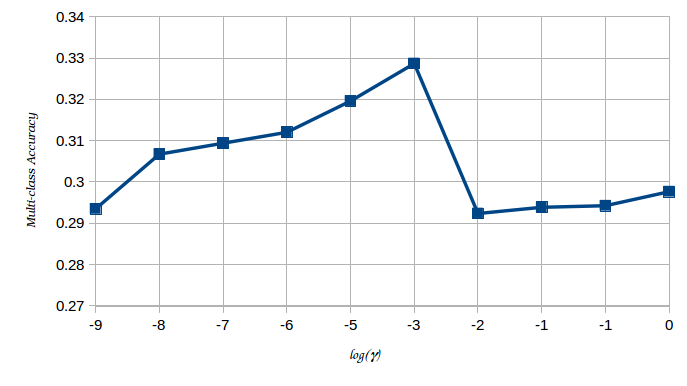
\includegraphics[width=\linewidth]{images/nn_param_apy}
    \caption{aPY}
\end{subfigure}
%
\begin{subfigure}[b]{0.43\linewidth}
    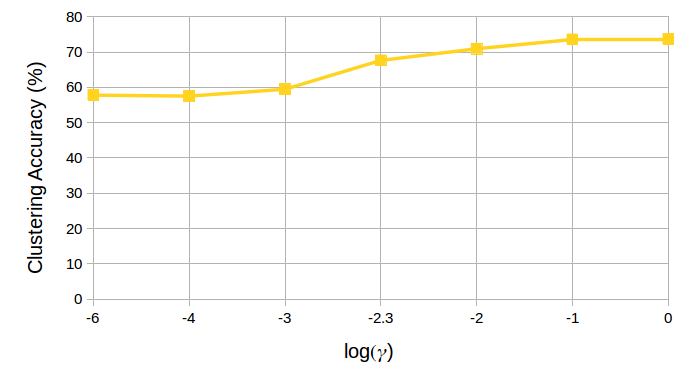
\includegraphics[width=\linewidth]{images/nn_gamma_awa}
    \caption{AwA}
\end{subfigure}
%
\begin{subfigure}[b]{0.43\linewidth}
    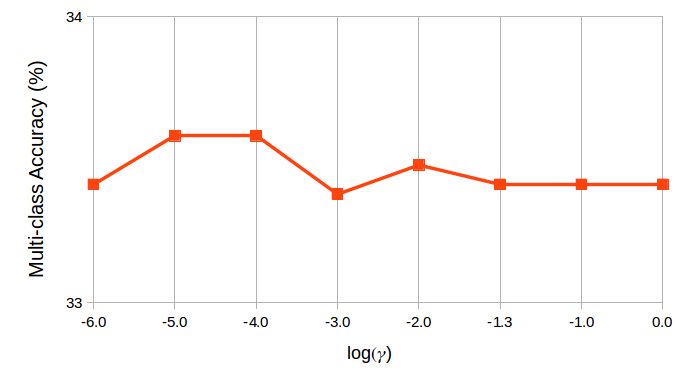
\includegraphics[width=\linewidth]{images/nn_param_birds}
    \caption{CUB-2011}
\end{subfigure}
\begin{subfigure}[b]{0.43\linewidth}
    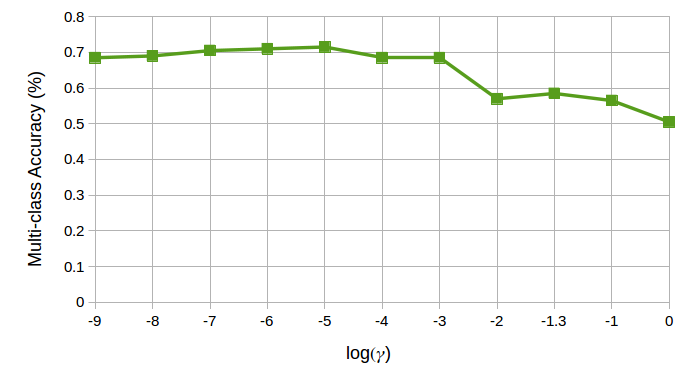
\includegraphics[width=\linewidth]{images/nn_param_sun}
    \caption{SUNA}
\end{subfigure}
\caption[نمودار تحلیل پارامتر شبکه عصبی]{
میزان دقت دسته‌بندی چند دسته‌ای در شبکه چندوظیفه‌ای ارائه شده (نسخه یک لایه) بر حسب $\log_{10}$ پارامتر $\gamma$ در معادله
\eqref{eq:nn_loss}.
}
\label{fig:nn_param}
\end{figure}




\section{بررسی خوشه‌بندی نیمه‌نظارتی}
\begin{table}[ht]
\centering
\caption[بررسی عمل‌کرد خوشه‌بندی نیمه‌نظارتی پیشنهاتی]{
امتیاز معیار دقت (٪) تخصیص خوشه‌ها که با رای‌گیری روی برچسب‌های صحیح به شماره دسته تبدیل شده است؛ بر روی چهار مجموعه داده مورد استفاده در یادگیری صفرضرب. نتایج روش پیشنهادی به صورت
\textit{ میانگین $\pm$ انحراف معیار }
برای سه اجرا گزارش شده‌است.}
\vspace*{2mm}
  \label{tab:clustering}
\begin{tabular}{|r|c|c|c|c|}
\hline
روش خوشه‌بندی & AwA & CUB-2011 & aPY & SUNA \\
\hline
k-means                             &  ${65.80}$                 & ${35.61}$           & ${65.37 }$               & ${17.49 }$   \\
\hline
خوشه‌بندی نیمه‌نظارتی (بخش \ref{clustering_method})
                      & \textbf{${70.74\pm 0.32}$}  & \textbf{${42.63\pm 0.07}$} & \textbf{${69.93\pm 3.4}$} & \textbf{ ${45.50 \pm 1.32}$} \\
\hline
\end{tabular}
\vspace{2mm}
\end{table}

در این بخش به بررسی عمل‌کرد روش خوشه‌بندی نیمه‌نظارتی ارائه شده در بخش \ref{clustering_method} می‌پردازیم. برای این منظور روش ارائه شده را روی هر مجموعه داده اجرا کرده، خوشه‌های مربوط به دسته‌های دیده‌شده را کنار گذاشته  و هر یک از خوشه‌های دیگر را به یک دسته از دسته‌های آزمون نسبت می‌دهیم. برای این کار در هر خوشه بر اساس برچسب صحیح نمونه‌ها رای‌گیری می‌شود و برچسبی که بیشتر اعضای آن خوشه آن را دارا هستند به کل اعضای خوشه نسبت داده می‌شود. نتیجه با برچسب‌های صحیح مقایسه شده و \gls{mulit-class-accurary} در جدول \ref{tab:clustering} گزارش شده است.
 برای مقایسه عمل‌کرد، آزمایش مشابهی را با روش \lr{k-means} اجرا می‌کنیم. به این صورت که  الگوریتم \lr{k-means} را با $k=n_s + 2n_u$ اجرا کرده و با هر خوشه با رای‌گیری برچسب یکی از دسته‌های دیده نشده را نسبت می‌دهیم. نتایج مربوط به این آزمایش نیز در جدول \ref{tab:clustering} گزارش شده است.

 در آزمایش‌های فوق پارامترهای $k$ و $\beta$ در رابطه \eqref{eq:my_clustering} توسط قواعد سرانگشتی ارائه شده در بخش \ref{simple_opt} تنظیم شده‌اند. برای روشن شدن میزان تاثیر این پارامترها در عمل‌کرد این روش خوشه‌بندی، دقت حاصل شده در این خوشه‌بندی بر اساس هر کدام از این پارامترها سنجیده شده و نتیجه در تصویر \ref{fig:cluster_params} ارائه شده است.
 همان‌طور که دیده می‌شود افزایش تعداد خوشه‌ها باعث افزایش دقت خوشه‌بندی  (با تعریف ارائه شده در بالا) شده است. باید به این نکته توجه کرد که این سیر صعودی طبیعی است و الزاما به معنای عمل‌کرد بهتر روش با تعداد خوشه‌های بیشتر نیست. در حقیقت، در حالت حدی بدیهی، وقتی تعداد خوشه‌ها با تعداد نمونه‌ها برابر شود دقت خوشه‌بندی به ۱ خواهد رسید. چرا که در این حالت هر خوشه تنها یک عضو دارد و با رای‌گیری روی برچسب اعضا، تنها رای همان عضو که برچسب صحیح خود است وجود دارد و در نتیجه تمام خوشه‌ها برچسب صحیحی دریافت خواهند کرد. با توجه به این مسئله، تنظیم این پارامتر با استفاده از اعتبارسنجی روی دقت خوشه‌بندی امکان پذیر نیست چرا که جواب بهینه‌ی آن یک حالت بدیهی خواهد بود. در عوض با توجه به استفاده‌ی ما از این روند خوشه‌بندی در دسته‌بندی صفرضرب، این پارامتر باید با توجه به تاثیرش بر دقت دسته‌بندی صفرضرب تنظیم شود. در این حالت همان‌طور که نتایج بخش \ref{exp:simple} نشان می‌دهد، دقت دسته‌بندی حساسیت کمی به تعداد خوشه‌ها دارد در نتیجه برای کاهش زمان آموزش توسط یک قاعده سرانگشتی تعیین خواهد شد.
 تاثیر مقدار پارامتر $\beta$ در دقت خوشه‌بندی نیز در  سمت راست تصویر \ref{fig:cluster_params} قابل مشاهده است، علاوه بر این تاثیر این پارامتر روی دقت نهایی دسته‌بندی صفرضرب نیز در بخش \ref{exp:simple} مورد بررسی قرار می‌گیرد. در این پژوهش برای ساده نگه داشتن روش با توجه به تاثیر نه چندان محسوس این پارامتر از اعتبار سنجی روی مقدار این پارامتر نیز صرف‌نظر شده است. امکان تعیین مقدار این اعتبار سنجی دقیقا با روند شرح داده شده در بخش \ref{exp:validation} امکان‌پذیر است و تنها بایست مقادیر کاندید به مجموعه جستجو اضافه شود.
  \begin{figure}[!h]
  \centering
  \begin{subfigure}[b]{0.43\linewidth}
    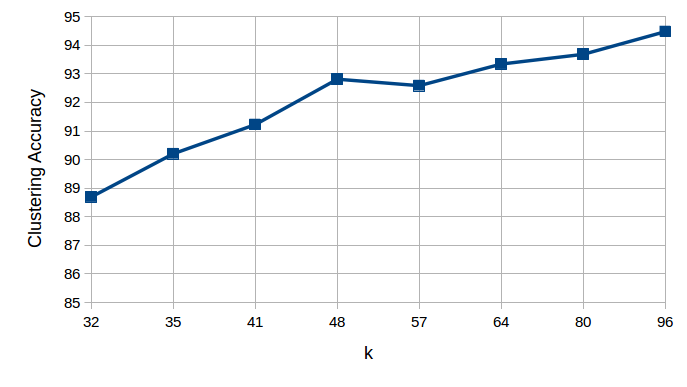
\includegraphics[width=\linewidth]{images/cluster_k_apy}
    % \caption{\lr{aPY, k}}
  \end{subfigure}
%
  \begin{subfigure}[b]{0.43\linewidth}
    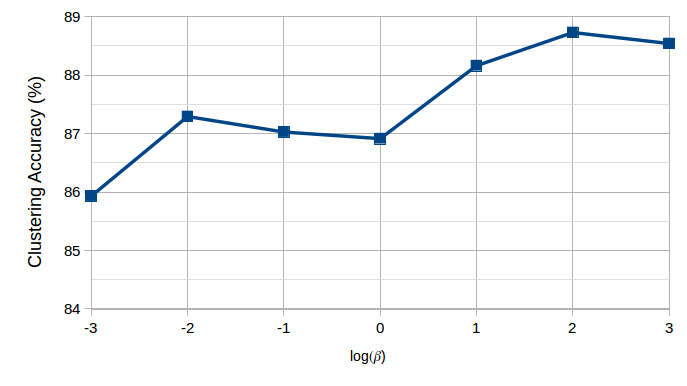
\includegraphics[width=\linewidth]{images/cluster_beta_apy}
    % \caption{\lr{aPY, $log(\beta)$}}
  \end{subfigure}
    \begin{subfigure}[b]{0.43\linewidth}
    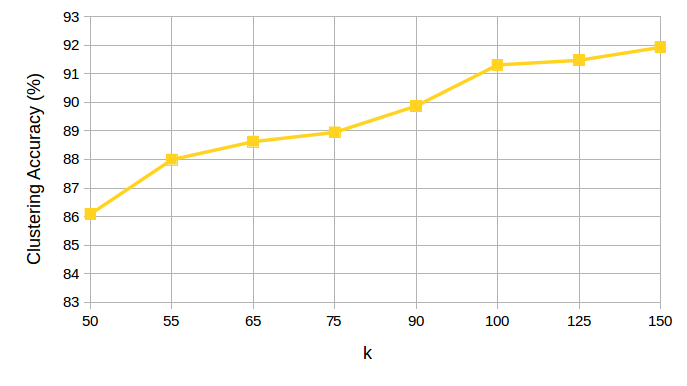
\includegraphics[width=\linewidth]{images/cluster_k}
    % \caption{\lr{AwA, k}}
  \end{subfigure}
    \begin{subfigure}[b]{0.43\linewidth}
    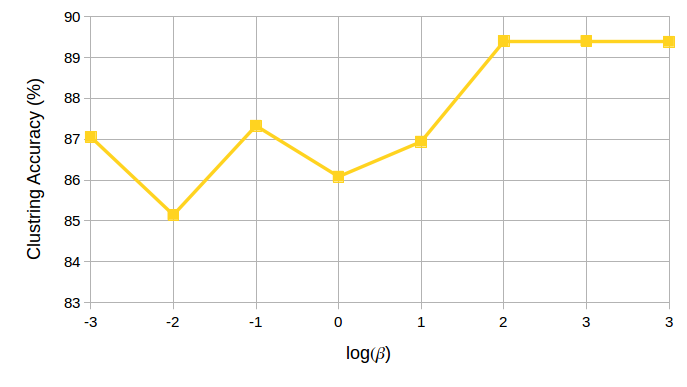
\includegraphics[width=\linewidth]{images/cluster_beta}
    % \caption{\lr{AwA, $log(\beta)$}}
  \end{subfigure}
    \begin{subfigure}[b]{0.43\linewidth}
    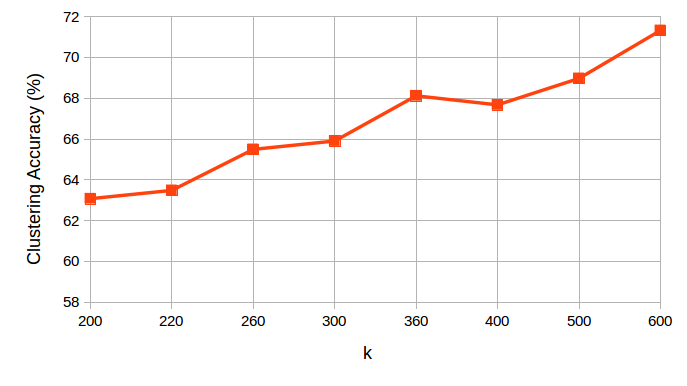
\includegraphics[width=\linewidth]{images/cluster_k_birds}
    % \caption{\lr{CUB-2011, k}}
  \end{subfigure}
    \begin{subfigure}[b]{0.43\linewidth}
    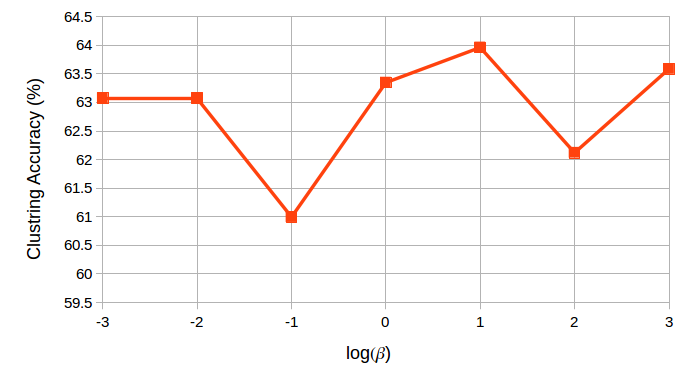
\includegraphics[width=\linewidth]{images/cluster_beta_birds}
    % \caption{\lr{CUB-2011, $log(\beta)$}}
  \end{subfigure}
    \begin{subfigure}[b]{0.43\linewidth}
    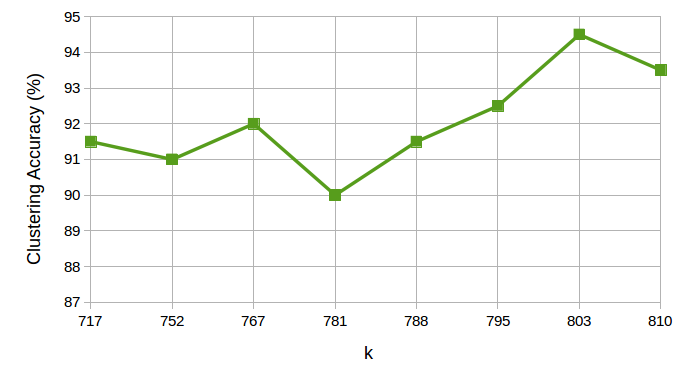
\includegraphics[width=\linewidth]{images/cluster_k_sun}
  \end{subfigure}
    \begin{subfigure}[b]{0.43\linewidth}
    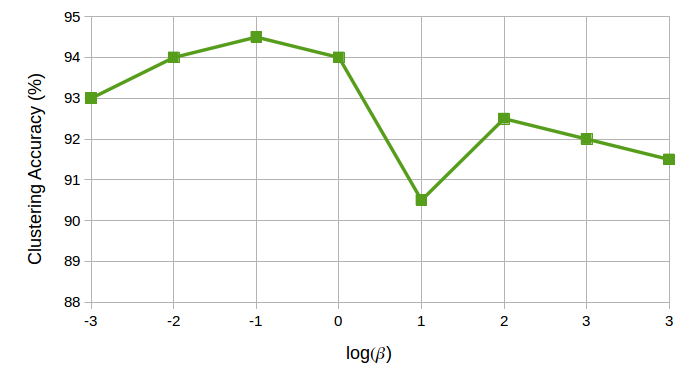
\includegraphics[width=\linewidth]{images/cluster_beta_sun}
    % \caption{\lr{SUNA $log(\beta)$}}
  \end{subfigure}
%

  \caption[تحلیل پارامترهای روش یادگیری نگاشت و خوشه‌بندی توام]{
  تاثیر پارامترهای  روش خوشه‌بندی نیمه‌نظارتی.
\textbf{سمت چپ}:
  نتیجه دقت خوشه‌بندی با تغییر تعداد خوشه‌های در نظر گرفته شده.
 \textbf{سمت راست}:
 نتیجه دقت  دسته‌بندی چند خوشه‌بندی بر حسب مقادیر پارامتر $\beta$ در رابطه \eqref{eq:my_clustering}.\\
 برای راحتی مقایسه محور عمودی  همه‌ی نمودارها با بازه‌های یک درصدی تقسیم‌بندی شده‌اند.\\
سطر اول (آبی‌رنگ): مجموعه دادگان \lr{aPY}. سطر دوم (زرد رنگ): مجموعه دادگان \lr{AwA}. سطر سوم (قرمز رنگ): مجموعه دادگان \lr{CUB-2011}. سطر چهارم (سبز رنگ): مجموعه دادگان \lr{SUNA}.
%مشاهده توام تاثیر هر دو پارامتر.
% نتایج نمودارها مربوط به مجموعه دادگان \lr{Animals with Attributes} است.
 }
  \label{fig:cluster_params}
  \end{figure}


\section{دسته‌بندی ساده با تابع مطابقت مبتنی بر خوشه‌بندی} \label{exp:simple}
در این بخش به بررسی عملی روش پیشنهادی برای دسته‌بندی با خوشه‌بندی و تابع مطابقت می‌پردازیم که  در بخش \ref{simple_method} معرفی شد و مراحل آن در الگوریتم \ref{alg:simple} ذکر شده است. این روش مبتنی بر یک خوشه‌بندی روی داده‌های آزمون بود و با استفاده از یک نگاشت خطی از فضای توصیف دسته‌ها به فضای تصاویر، مرکز هر خوشه را به یک دسته‌ی دیده نشده منتسب می‌کرد. بر اساس تابع مطابقت پیشنهادی (بخش \ref{compatibility_function})، تمام اعضای هر خوشه همان برچسبی که مرکزشان دریافت کرده را دریافت می‌کند.

این روش با استفاده از دو نوع خوشه‌بندی آزمایش شده است. یکی خوشه‌بندی نیمه‌نظارتی پیشنهادی که نتایج این حالت با عنوان
\textit{پیشنهادی (خوشه‌بندی نیمه‌نظارتی + تابع مطابقت) }
در جدول \ref{tab:results} آمده است.
 برای بررسی تاثیر خوشه‌بندی ارائه شده یک نسخه دیگر از این روش که در آن از خوشه‌بندی \lr{k-means} بجای خوشه‌بندی پیشنهادی استفاده شده است نیز مورد آزمایش قرار گرفته است. نتایج مربوط به این روش با عنوان
\textit{ پیشنهادی (تابع مطابقت + \lr{k-means} ) }
آمده است. نتایج ارائه شده حاصل سه بار اجرا هستند که به صورت
\textit{ میانگین $\pm$ انحراف معیار }
بیان شده‌اند. همان‌گونه که از نتایج مشخص است، استفاده از خوشه‌بندی نیمه‌نظارتی ارائه شده همواره نتایج بهتری نسبت به استفاده از خوشه‌بندی  \lr{k-means} تولید خواهد کرد.

 تاثیر پارامترهای مورد استفاده در این قسمت در شکل \ref{fig:simple_params} آمده است. همان‌طور که مشاهده می‌شود \gls{hyperparameter} $\eta$ در رابطه
 \eqref{eq:d_answer}
تاثیر قابل توجهی بر دقت دسته‌بندی نهایی دارد، در نتیجه ما مقدار این \gls{hyperparameter} را با استفاده از روند اعتبارسنجی شرح داده شده در بخش \ref{exp:validation} تنظیم کرده‌ایم. از طرف دیگر مشاهده می‌شود تعداد خوشه‌ها در خوشه‌بندی نیمه‌نظارتی ارائه شده تاثیر قابل توجهی بر دقت دسته‌بندی ندارد، در نتیجه برای سادگی و کاهش زمان روند آموزش ما این \gls{hyperparameter} را همان‌طور که در بخش
 \ref{clustering_method}
 شرح داده شد با استفاده از یک قاعده سرانگشتی بر حسب تعداد دسته‌ها تعیین می‌کنیم که تعداد خوشه‌ها برای هر مجموعه داد‌ه‌گان برابر $k = n_s + 2n_u$ در نظر گرفته می‌شود.

 \begin{figure}[!h]
   \captionsetup[subfigure]{labelformat=empty, font=footnotesize}
  \centering
  \begin{subfigure}[b]{0.3\linewidth}
    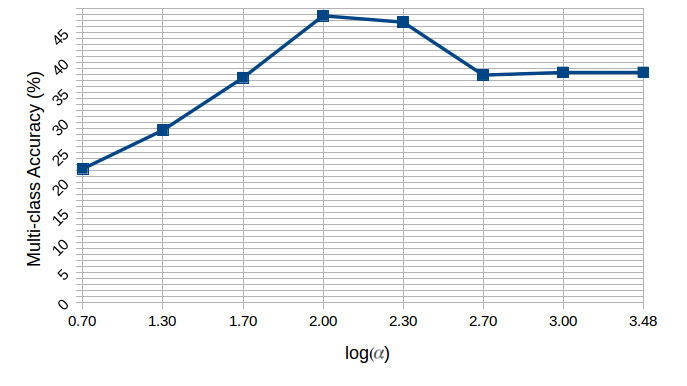
\includegraphics[width=\linewidth]{images/simple_gamma}
  \end{subfigure}
  \begin{subfigure}[b]{0.3\linewidth}
    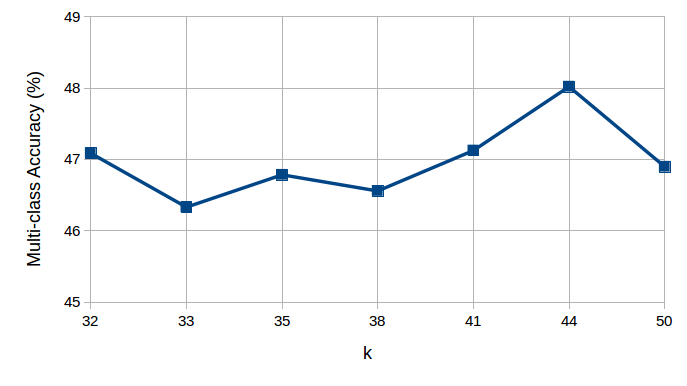
\includegraphics[width=\linewidth]{images/simple_k}
  \end{subfigure}
    \begin{subfigure}[b]{0.3\linewidth}
    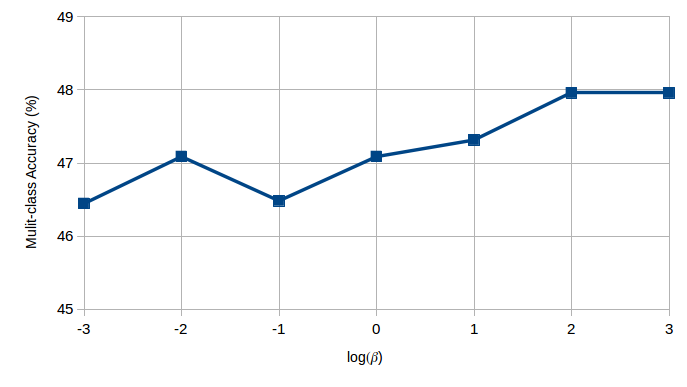
\includegraphics[width=\linewidth]{images/simple_beta}
  \end{subfigure}
  %%%%%%%%%%%%
    \begin{subfigure}[b]{0.3\linewidth}
    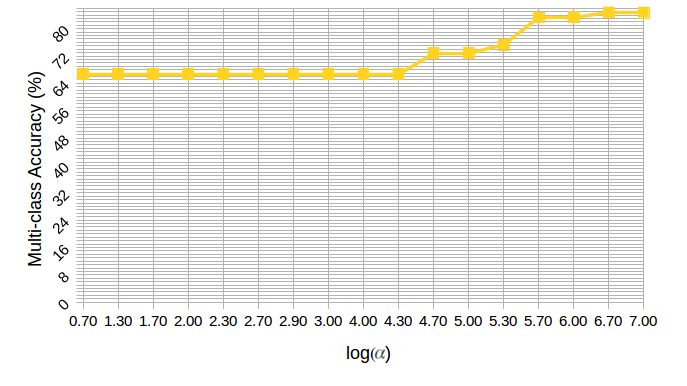
\includegraphics[width=\linewidth]{images/simple_gamma_awa}
  \end{subfigure}
  \begin{subfigure}[b]{0.3\linewidth}
    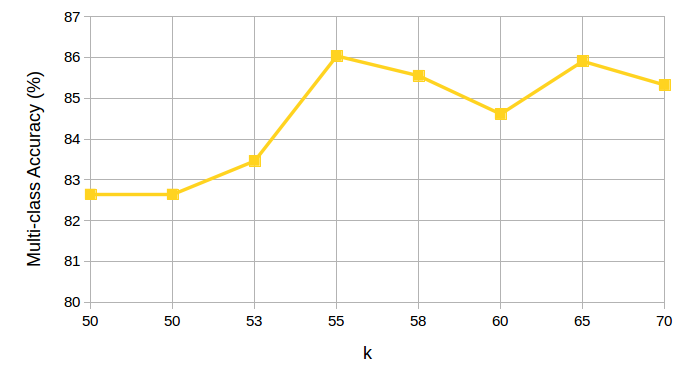
\includegraphics[width=\linewidth]{images/simple_k_awa}
  \end{subfigure}
    \begin{subfigure}[b]{0.3\linewidth}
    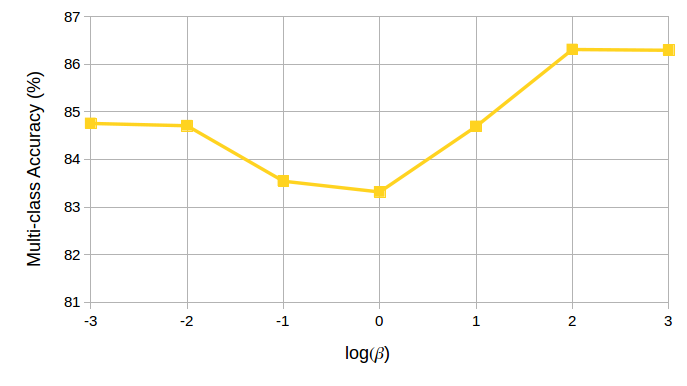
\includegraphics[width=\linewidth]{images/simple_beta_awa}
  \end{subfigure}
  %
    \begin{subfigure}[b]{0.3\linewidth}
    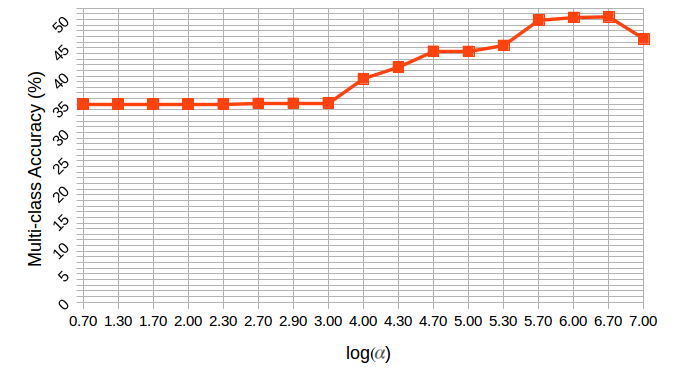
\includegraphics[width=\linewidth]{images/simple_gamma_birds.png}
  \end{subfigure}
  \begin{subfigure}[b]{0.3\linewidth}
    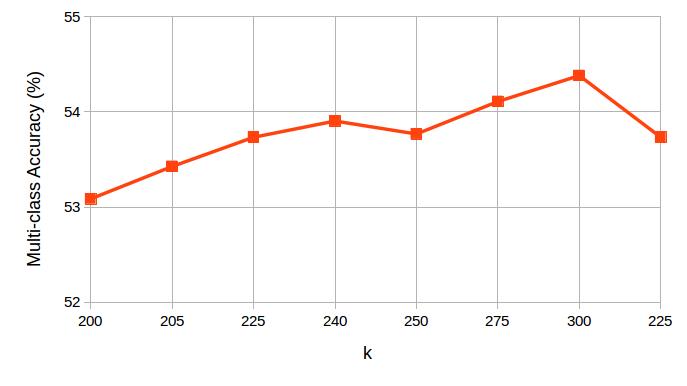
\includegraphics[width=\linewidth]{images/simple_k_birds.png}
  \end{subfigure}
    \begin{subfigure}[b]{0.3\linewidth}
    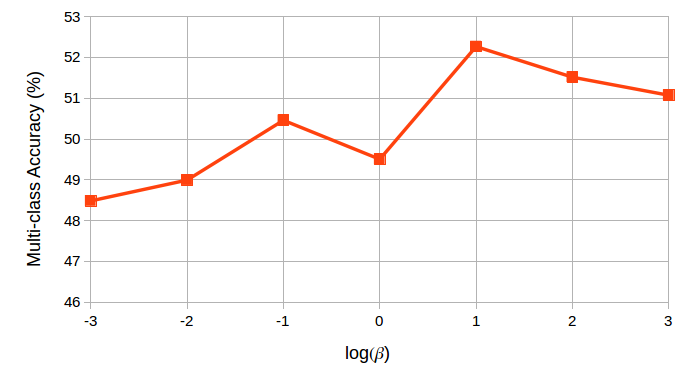
\includegraphics[width=\linewidth]{images/simple_beta_birds.png}
  \end{subfigure}
  %%00000000000000000000000000000
    \begin{subfigure}[b]{0.3\linewidth}
    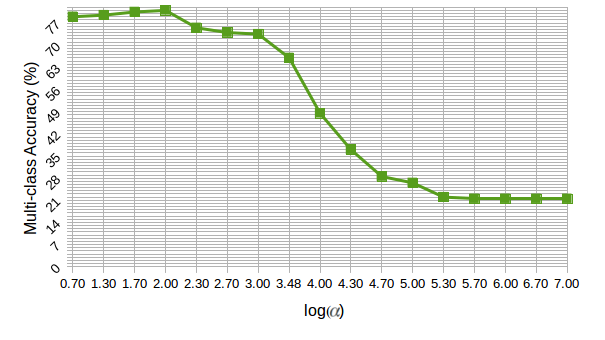
\includegraphics[width=\linewidth]{images/simple_gamma_sun.png}
  \end{subfigure}
  \begin{subfigure}[b]{0.3\linewidth}
    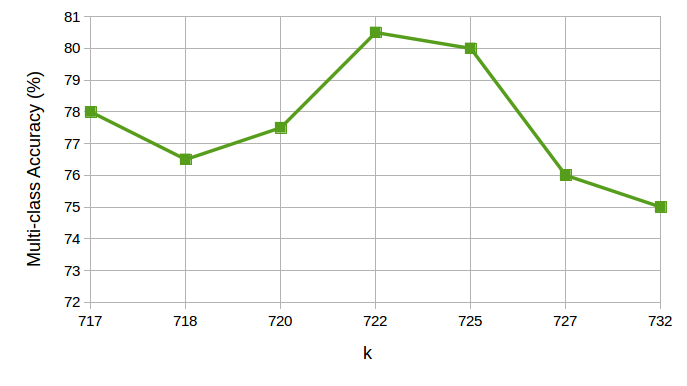
\includegraphics[width=\linewidth]{images/simple_k_sun}
  \end{subfigure}
  \begin{subfigure}[b]{0.3\linewidth}
    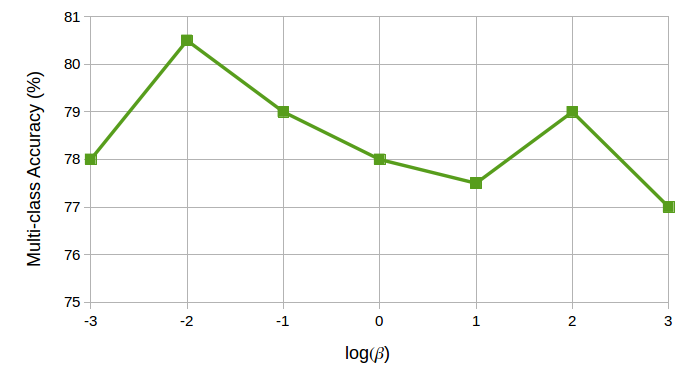
\includegraphics[width=\linewidth]{images/simple_beta_sun}
  \end{subfigure}
  \caption[تحلیل پارامترهای روش دسته‌بندی با خوشه‌بندی نیمه‌نظارتی]{
  تاثیر پارامترهای  روش دسته‌بندی با خوشه‌بندی نیمه‌نظارتی.    \textbf{سمت چپ}: نتیجه دقت دسته‌بندی چند دسته‌ای بدست آمده بر حسب \gls{hyperparameter}  $\alpha$ در رابطه
 \eqref{eq:d_answer}
 که اهمیت جمله منظم‌سازی را نشان می‌دهد. همان‌طور که مشاهده می‌شود، عمل‌کرد روش به این \gls{hyperparameter} حساس است.
 \textbf{وسط }:
 نتیجه دقت  دسته‌بندی چند دسته‌ای بدست آمده بر حسب تعداد خوشه‌ها در خوشه‌بندی نیمه‌نظارتی. با توجه مقیاس این نمودار مشخص می‌شود که دقت حاصل شده حساسیت کمی نسبت به این پارامتر دارد.
  \textbf{سمت راست}:
  نتیجه دقت دسته‌بندی چنددسته‌بای بر حسب پارامتر $\beta$ در خوشه‌بندی نیمه نظارتی (رابطه \eqref{eq:my_clustering}).\\
  برای راحتی مقایسه محور عمودی  همه‌ی نمودارها با بازه‌های یک درصدی تقسیم‌بندی شده‌اند.\\
سطر اول (آبی‌رنگ): مجموعه دادگان \lr{aPY}. سطر دوم (زرد رنگ): مجموعه دادگان \lr{AwA}. سطر سوم (قرمز رنگ): مجموعه دادگان \lr{CUB-2011}. سطر چهارم (سبز رنگ): مجموعه دادگان \lr{SUNA}.
 }
  \label{fig:simple_params}
  \end{figure}




\section{ خوشه‌بندی و یادگیری نگاشت توام}\label{exp:jeac}
\label{exp:cluster}
روش پیشنهادی دوم که در بخش \ref{jeac} ارائه شد به خوشه‌بندی و یادگیری نگاشت توام می‌پرداخت و برچسب نمونه‌های آزمون در آن به طور مستقیم در جریان آموزش بدست می‌آید.
تنظمیات آزمایش برای روش خوشه‌بندی و نگاشت توام مانند حالت قبل سه بار اجرا و گزارش نتایج به صورت \textit{ میانگین $\pm$ انحراف معیار } است. دو نوع  مقداردهی اولیه انجام شده است. یکی همان‌طور که در بخش \ref{jeac} بیان شد، مقداردهی $R$ که با استفاده از الگوریتم
\ref{alg:simple}
انجام می‌شود. نتایج مربوط به این حالت در جدول  \ref{tab:results} با عنوان
\textit{ پیشنهادی (توام، مقداردهی $R$)}
آمده‌اند. یک مقداردهی دیگر شروع بهینه‌سازی تناوبی در الگوریتم
\ref{alg:jeac}
 با مقداردهی $D$ است که توسط رابطه
\eqref{eq:d_answer}
صورت گرفته است. نتایج مربوط به این حالت با عنوان
\textit{پیشنهادی (توام، مقداردهی $D$)}
آمده‌اند. مقایسه نتایج مربوط به این دو نحوه‌ی مقداردهی اولیه نشان می‌دهد که استفاده از روش پیشنهادی الگوریتم \ref{alg:simple}  برای رسیدن به دقت بالا ضروری است، چرا که مشاهده می‌شود که استفاده از مقداردهی اولیه برای $R$ به صورت بیان شده در الگوریتم \ref{alg:jeac} به طور متوسط $6.8$٪ دقت بالاتری در دسته‌بندی نسبت به مقداردهی $D$  با رابطه \eqref{eq:d_answer} دارد. دلیل این موضوع همان‌طور که در بخش \ref{jeac} بیان شد استفاده از اطلاعات بدون نظارت نمونه‌های آزمون در بدست آوردن مقدار اولیه برای $R$ است در حالیکه در مقداردهی اولیه $D$ تنها نمونه‌های آموزش دخالت دارند.

به علت حساسیت نتایج این روش به پارامترهای آن  (مقادیر  $\lambda$ و $\eta$ در رابطه \eqref{eq:joint})، مقادیر آن‌ها توسط روند اعتبارسنجی شرح داده شده در بخش
\ref{exp:validation}
تنظیم می‌شود. میزان تاثیر مقادیر این دو پارامتر در نتیجه روش در تصویر \ref{fig:jeac_params} نشان داده شده است. در نمودارهای ارائه شده معیار دقت دسته‌بندی چنددسته‌ای بر حسب مقادیر این دو پارامتر ترسیم شده‌اند.
 \begin{figure}[!h]
   \captionsetup[subfigure]{labelformat=empty, font=footnotesize}
  \centering
  \begin{subfigure}[b]{0.43\linewidth}
    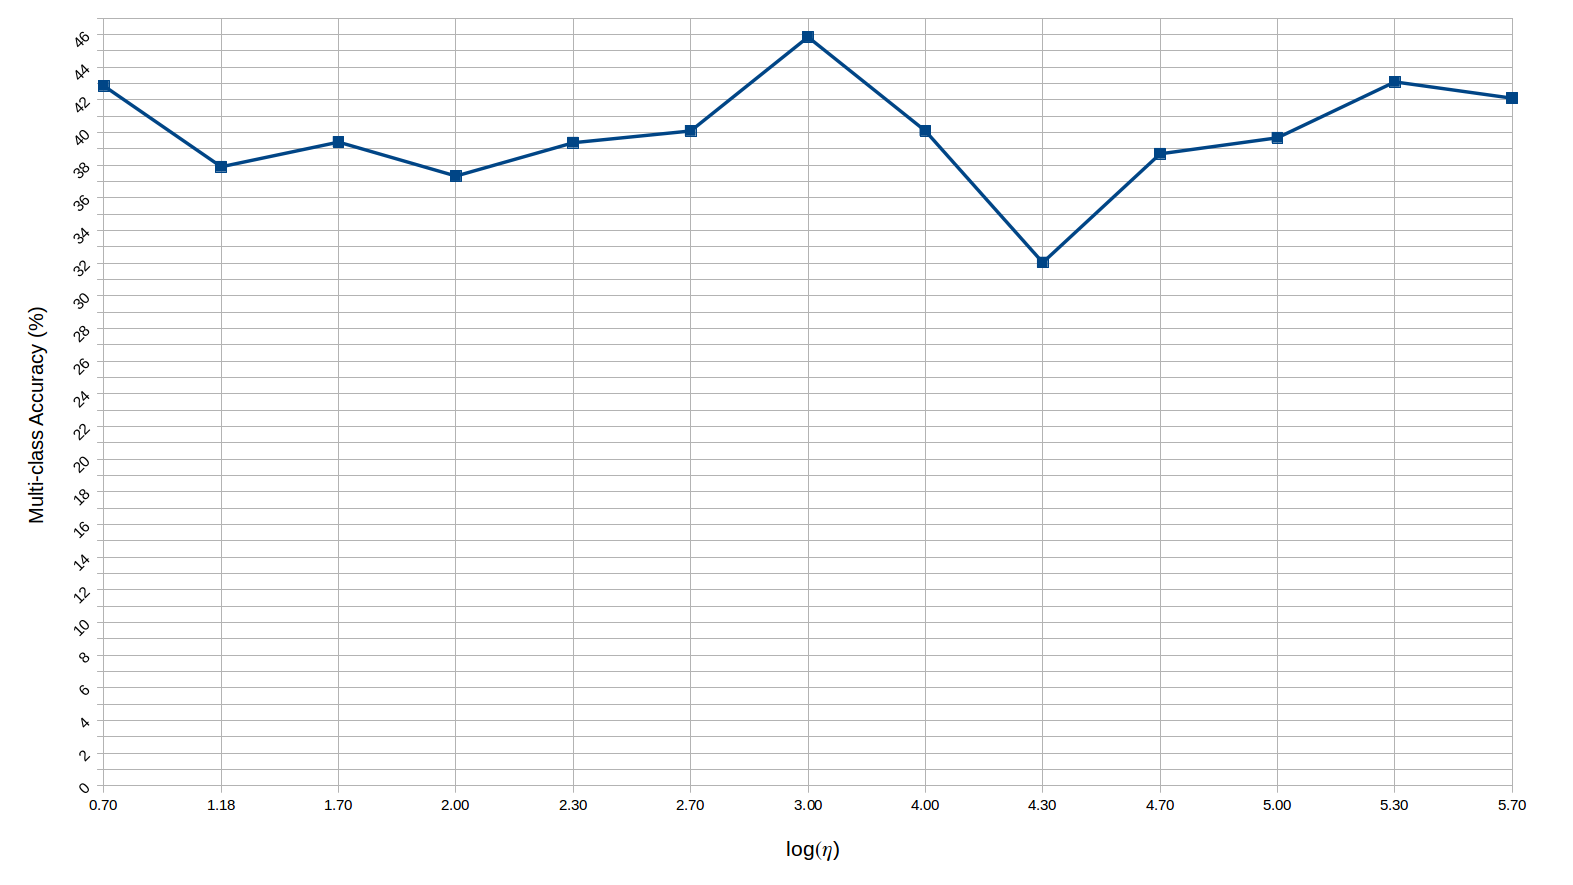
\includegraphics[width=\linewidth]{images/jeac_gamma}
  \end{subfigure}
  \begin{subfigure}[b]{0.43\linewidth}
    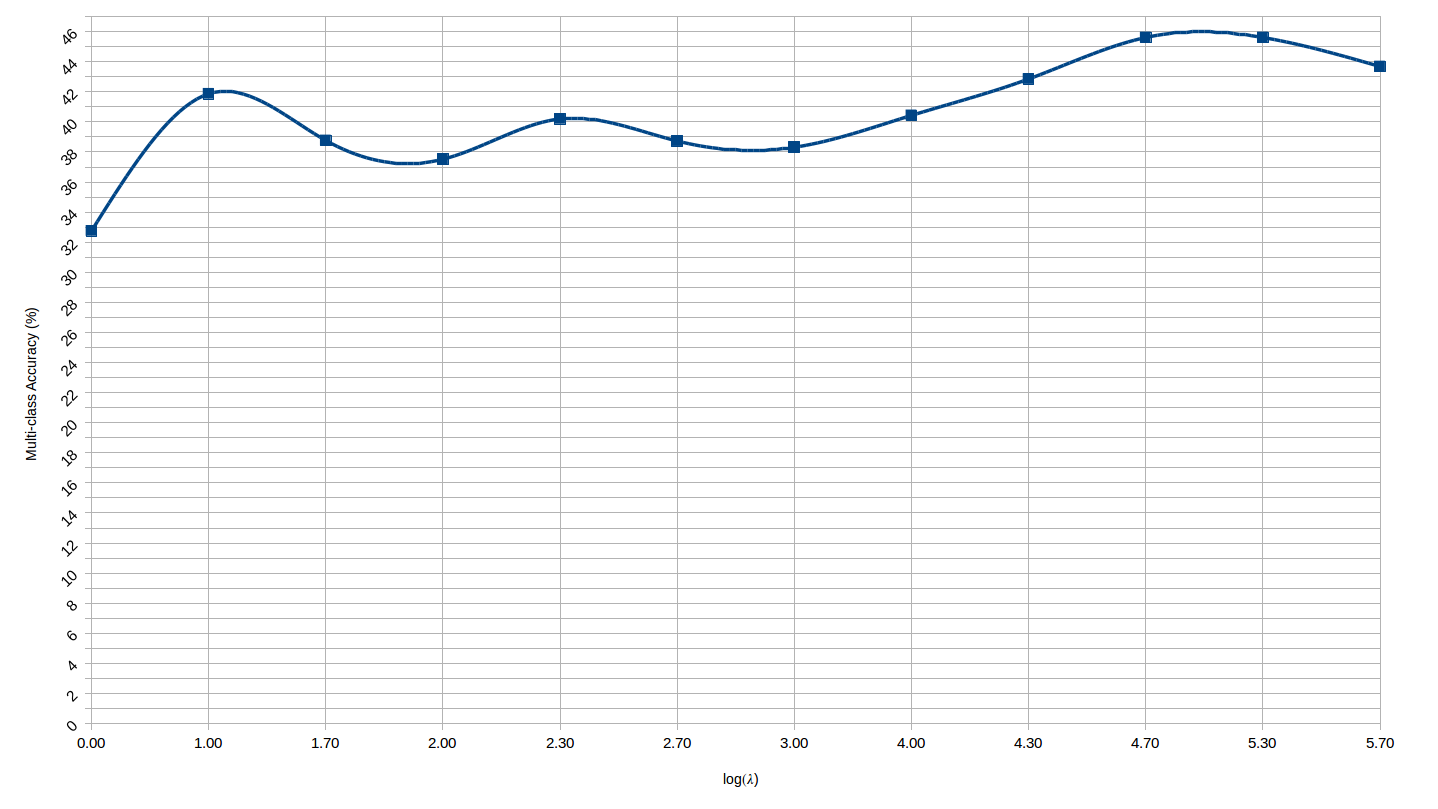
\includegraphics[width=\linewidth]{images/jeac_lambda}
  \end{subfigure}
  %%%%%%%%%%%%
    \begin{subfigure}[b]{0.43\linewidth}
    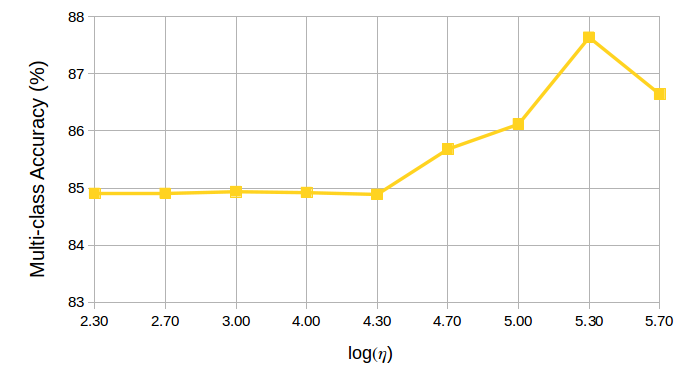
\includegraphics[width=\linewidth]{images/jeac_gamma_awa}
  \end{subfigure}
    \begin{subfigure}[b]{0.43\linewidth}
    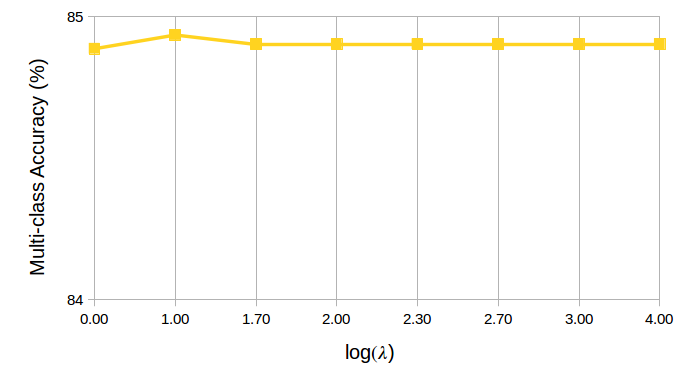
\includegraphics[width=\linewidth]{images/jeac_lambda_awa}
  \end{subfigure}
  %
    \begin{subfigure}[b]{0.43\linewidth}
    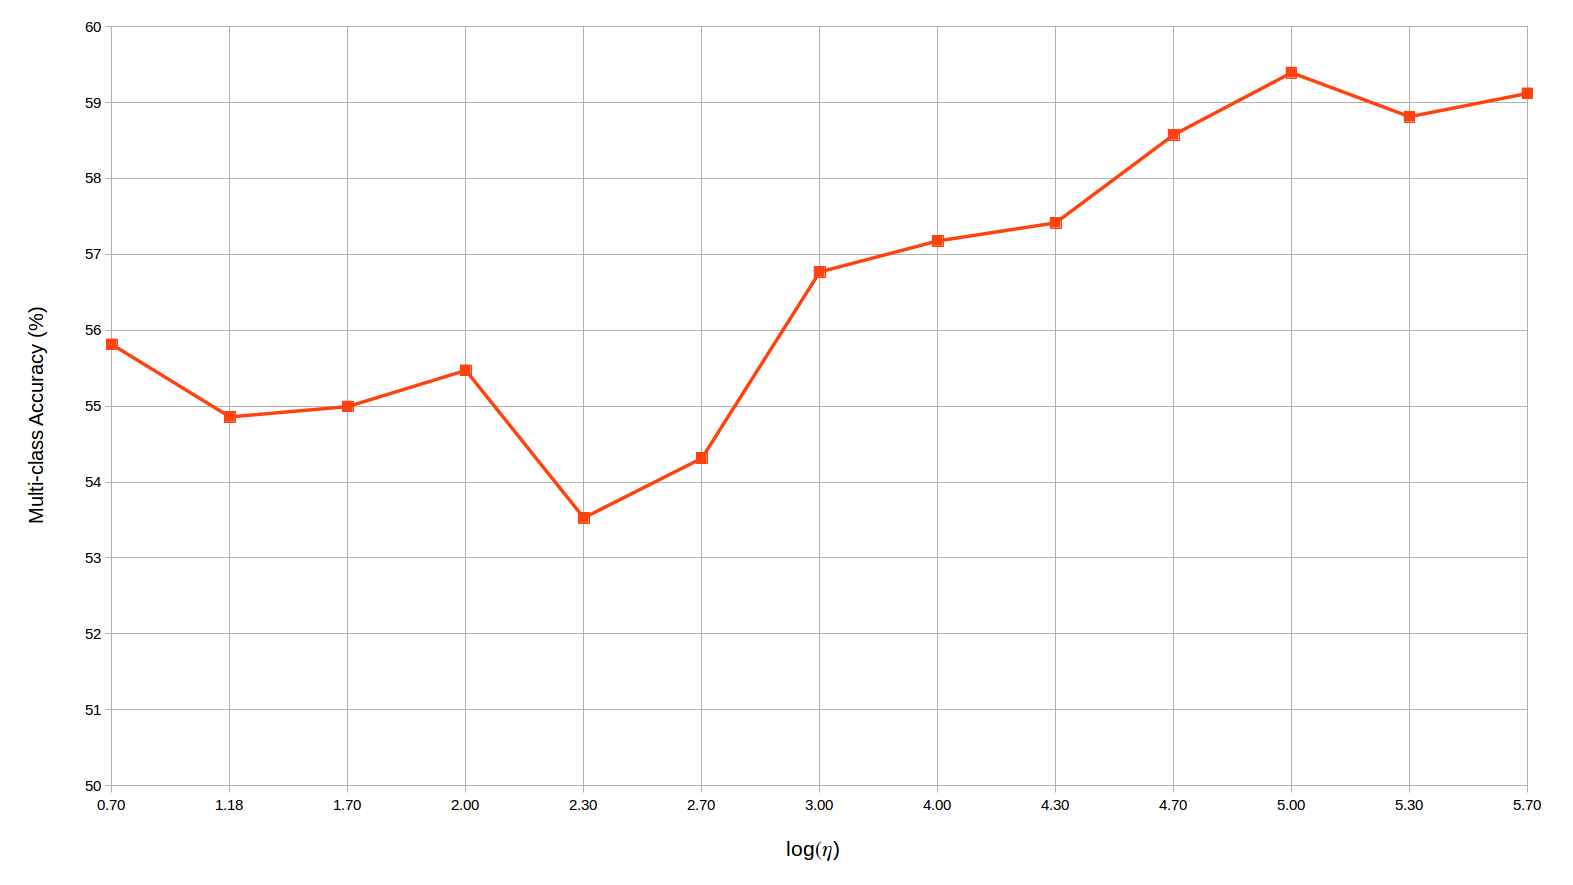
\includegraphics[width=\linewidth]{images/jeac_gamma_birds.png}
  \end{subfigure}
\begin{subfigure}[b]{0.43\linewidth}
    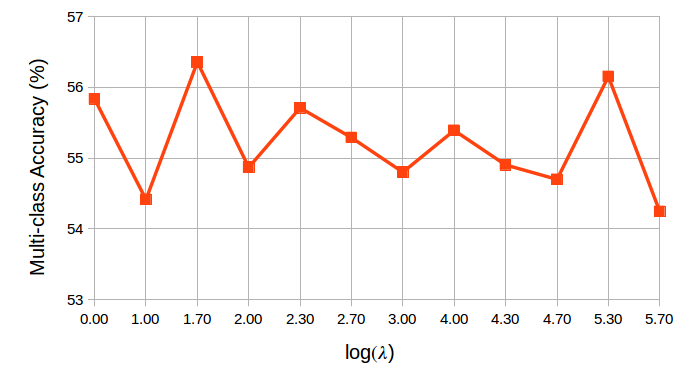
\includegraphics[width=\linewidth]{images/jeac_lambda_birds.png}
  \end{subfigure}
  %%00000000000000000000000000000
    \begin{subfigure}[b]{0.43\linewidth}
    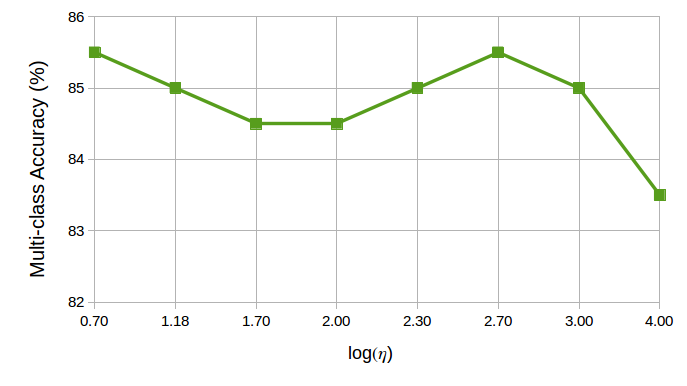
\includegraphics[width=\linewidth]{images/jeac_gamma_sun.png}
  \end{subfigure}
  \begin{subfigure}[b]{0.43\linewidth}
    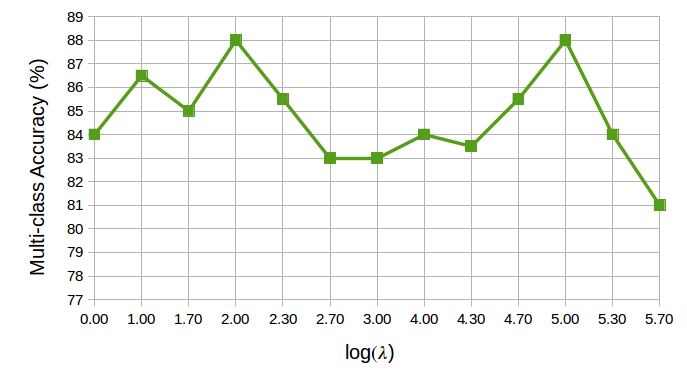
\includegraphics[width=\linewidth]{images/jeac_lambda_sun}
  \end{subfigure}
  \caption[تحلیل پارامترهای روش یادگیری نگاشت و خوشه‌بندی توام]{
  تاثیر پارامترهای  روش یادگیری نگاشت و خوشه‌بندی نیمه‌نظارتی برای مجموعه دادگان مختلف.
\textbf{سمت چپ:}
   نتیجه دقت دسته‌بندی چند دسته‌ای بدست آمده بر حسب \gls{hyperparameter}  $\nu$ در رابطه
\eqref{eq:joint}
 که اهمیت جمله منظم‌سازی را نشان می‌دهد.
 % همان‌طور که مشاهده می‌شود، عمل‌کرد روش به این \gls{hyperparameter} حساس است.
 \textbf{سمت راست}:
 نتیجه دقت  دسته‌بندی چند دسته‌ای بدست آمده بر حسب مقادیر پارامتر $\lambda$ در رابطه \eqref{eq:joint}
برای راحتی مقایسه محور عمودی  همه‌ی نمودارها با بازه‌های یک درصدی تقسیم‌بندی شده‌اند.\\
سطر اول (آبی‌رنگ): مجموعه دادگان \lr{aPY}. سطر دوم (زرد رنگ): مجموعه دادگان \lr{AwA}. سطر سوم (قرمز رنگ): مجموعه دادگان \lr{CUB-2011}. سطر چهارم (سبز رنگ): مجموعه دادگان \lr{SUNA}.
 }
  \label{fig:jeac_params}
  \end{figure}

\subsection{روش‌های مورد مقایسه}\label{exp:other_methods}
در این بخش قصد داریم روش‌های پیشنهادی در بخش‌های \ref{simple_method} و \ref{jeac} را با مطرح‌ترین روش‌های اخیر در حوزه یادگیری صفرضرب مقایسه کنیم.
سایر روش‌هایی که در جدول  \ref{tab:results} برای مقایسه آورده شده‌اند، روش‌هایی هستند که بالاترین دقت‌های دسته‌بندی را در دسته‌بندی صفرضرب با استفاده از توصیف‌های به صورت بردار صفت دارا هستند.
روش‌های ارائه شده در
\cite{li15max, semi15, Kodirov2015}
از این جهت که \textit{نیمه‌نظارتی} هستند، یعنی از  نمونه‌های آزمون نیز در زمان آموزش استفاده می‌کنند، با روش‌های ما بیشترین نزدیکی را دارند. البته در
\cite{li15max, semi15}
از ویژگی‌های کم‌عمق برای تصاویر استفاده شده است که توانایی جداسازی دسته‌ها در آن بسیار پایین‌تر از ویژگی‌های بدست آمده از شبکه‌های عصبی ژرف است که در روش‌های پیشنهادی ما مورد استفاده قرار گرفته است. روش‌های
\cite{Akata2015, Xian2016}
با استفاده از توابع هزینه‌ی بیشترین حاشیه سعی در یادگیری نگاشت از هر دو فضای تصاویر و توصیف دسته‌ها به فضای مشترک دارند. این روش‌ها از ویژگی‌های شبکه‌ی ژرف
\lr{GoogleNet}
 \cite{googlenet}
 برای استخراج ویژگی استفاده می‌کنند. ابعاد ویژگی‌های بدست آمده ۱۰۲۴ است که بعد کمتری نسبت به ویژگی‌های ۴۰۹۶-بعدی استخراج شده از شبکه ۱۹ لایه‌ی vgg دارد و توانایی جداسازی دسته‌ها در آن پایین‌تر است. همان‌طور که مشاهده می‌شود استفاده از این ویژگی‌های با بعد بیشتر عمل‌کرد روش ارائه شده در \cite{Akata2015} را بهبود داده است.

 روش‌هایی که بهترین نتایج را در میان روش‌های رقیب کسب کرده‌اند، روش ارائه شده در \cite{sse} و تعمیم آن در \cite{agnostic}  هستند. هرچند این روش‌ها نیمه‌نظارتی نیستند و تنها از نمونه‌های آموزش برای یادگیری نمایش تصاویر و توصیف دسته‌ها در یک فضای مشترک، که فضای هیستوگرام دسته‌های دیده شده است استفاده می‌کنند، نتایج بهتری نسبت به روش‌های نیمه‌نظارتی پیشین در \cite{li15max, semi15, Kodirov2015} کسب کرده‌اند. این مسئله می‌توان نشان‌گر یک مسیر مناسب در ترکیب روش پیشنهادی در این پژوهش با فضای مشترک مورد استفاده در آن روش‌ها برای کارهای آتی باشد.

\begin{table}[ht]
\caption [مقایسه دقت دسته‌بندی]{
مقایسه دقت دسته‌بندی چنددسته‌ای روش پیشنهادی با سایر روش‌ها. نتایج بر اساس نوع ویژگی مورد استفاده برای تصاویر دسته‌بندی شده‌اند. جدول شامل دقت دسته‌بندی چنددسته‌ای به صورت
(میانگین $\pm$ انحراف معیار) است. نتایج سایر روش‌ها از مقالاتی که روش در آن‌ها ارائه شده نقل شده و آزمایش‌ها توسط ما تکرار نشده است. نتایج روش‌های پیشنهادی حاصل سه اجرا هستند.
}
\vspace{4mm}
 \label{tab:results}
 {\footnotesize
\begin{tabular}{|r|r|c|c|c|c|}
\hline
ویژگی تصاویر & روش  & AwA & CUB-2011 & aPascal-aYahoo & SUN \\
\hline
{کم‌عمق}
& \lr{Li and Guo } \cite{li15max}                 &  $38.2 \pm 2.3$   &                 &                         & $18.9 \pm 2.5$ \\
& \lr{Li \textit{et al.}}~\cite{semi15}                    &  $40.05\pm 2.25$ &                 &   $24.71 \pm 3.19$       &     \\
& \lr{Jayaraman and Grauman}  \cite{jayaraman14}  & $43.01 \pm 0.07$ &                 & $26.02 \pm 0.05$        & $56.18 \pm 0.27$ \\
\hline
{GoogleNet}
& \lr{Akata \textit{et al.}}~\cite{Akata2015}              & $66.7$          & $50.1$            &                         & \\
%& \lr{Changpinyo \textit{et al.}}~\cite{Synthesized}       & $72.9$           & $54.5$            &                         & $62.7$ \\
& \lr{Xian \textit{et al.}}~\cite{Xian2016}                & $71.9$            & $45.5$            &                         & \\
\hline
{VGG-19}
&\lr{ Khodirov \textit{et al.}} \cite{Kodirov2015}
                                            & $73.2$            &  $39.5$           & $26.5$                    &  \\
& \lr{Akata \textit{et al.}}~\cite{Akata2015}              & $61.9$            &  $50.1$           &                         & \\
& \lr{Zhang and Saligrama}  \cite{sse}            &  $76.33 \pm 0.53$ & $30.41 \pm 0.20$ &   $46.23 \pm 0.53$      & $82.50 \pm 1.32$    \\
& \lr{Zhang and Saligrama} \cite{agnostic}       &  $80.46 \pm 0.53$ & $42.11 \pm 0.55$ &   \textbf{$50.35 \pm 2.97$}      & $83.83 \pm 0.29$    \\
&  پیشنهادی (تابع مطابقت + \lr{k-means})
                          & $86.34 \pm 0.13$               & $52.48 \pm 0.60$              & $48.03 \pm 1.56$              & $75.75 \pm 1.06$ \\
& پیشنهادی (تابع مطابقت + خوشه‌بندی نیمه‌نظارتی)
                        & $86.38 \pm 0.56$              & $ 53.10\pm 0.43 $             & $48.52 \pm 0.29$              &$ 80.66 \pm 0.76$ \\
& پیشنهادی (توام، مقداردهی $D$)
                     & $83.03$                        & $57.55$                       & $42.62$          & $72.50$\\
& پشنهادی (توام، مقداردهی $R$)
                     & \textbf{\em $88.64 \pm 0.04$}  & \textbf{\em $58.80 \pm 0.64$} & $49.77 \pm 2.02$ & \textbf{\em $86.16 \pm 0.57$} \\
\hline
\end{tabular}
}
\end{table}

\section{تحلیل نتایج}\label{exp:discussion}
با توجه به جدول \ref{tab:results} روش پیشنهادی یادگیری توام نگاشت و خوشه‌بندی هنگام مقداردهی اولیه مقادیر $R$ مجموعا به بهترین نتایج دست‌یافته است. این روش روی سه مجموعه داد‌ه‌گان از چهار مجموعه که روش‌ها با آن محک زده شده‌اند نتایج بهتری نسبت به سایر روش‌ها دارد و عمل‌کرد پیشگام در حوزه یادگیری صفرضرب را ارتقاء داده است. روی مجموعه داده‌گان \lr{aPascal/aYahoo} روش ارائه شده در 
\cite{agnostic}
نتایج بهتری کسب کرده است. دلیل این موضوع می‌تواند شباهت بسیار زیاد میان امضای دسته‌ها در این مجموعه دادگان و عدم ایجاد جداسازی بالا میان دسته‌ها توسط این بردارهای توصیف است. در روش پیشنهادی یادگیری نگاشت و خوشه‌بندی توام، با توجه به نزدیکی زیاد این بردارهای توصیف، نگاشت آن‌ها در فضای ویژگی تصاویر نیز به یکدیگر نزدیک خواهد بود و جداسازی مناسبی میان نمونه‌های دسته‌های مختلف صورت 
نمی‌پذیرد؛ ولی در روش ارائه شده در \cite{agnostic} همان‌گونه که در فصل دوم مرور شد، بردارهای توصیف ورودی 
مستقیماً به کار گرفته نمی‌شوند، بلکه از آن‌ها برای بدست آوردن نمایش دیگری برای دسته‌ها  به صورت هیستوگرامی از دسته‌های دیده شده، استفاده می‌شود. وجود این گام می‌تواند مشکل نزدیکی و شباهت زیاد میان امضای دسته‌ها را از بین ببرد. هم‌چنین همان‌طور که در بخش \ref{jeac_opt} بیان شد، مقداردهی اولیه مقادیر $R$ با استفاده از روش خوشه‌بندی و تابع مطابقت پیشنهادی عمل‌کرد بهتری نسبت به مقداردهی اولیه $D$ دارد. از این جدول هم‌چنین کارایی روش خوشه‌بندی نیمه‌نظارتی پیشنهادی نسبت به الگوریتم \lr{k-means} در مسئله یادگیری بدون برد مشخص می‌شود، چرا که در همه‌ی موارد هنگام استفاده از روش خوشه‌بندی نیمه‌نظارتی پیشنهادی در مقایسه با  الگوریتم \lr{k-means} دقت بالاتری در دسته‌بندی حاصل شده است. هر دو حالت این روش ساده که از یک نگاشت خطی و بخش تاثیرگذارتر تابع مطابقت پیشنهادی تشکیل شده‌اند، روی نیمی از چهار مجموعه‌داده‌گان مورد بررسی عمل‌کرد بهتری نسبت به همه‌ی روش‌های پیشین داشته‌اند که نشان‌دهنده کارایی تابع مطابقت پیشنهادی است.

برای تحلیل کارایی روش قسمت‌های مختلف آن و تاثیر هر یک  روی یک مجموعه داده واقعی در شکل
\ref{fig:discussion}
 نشان داده شده است. نتایج مربوط به اجرای روش روی تمام مجموعه دادگان AwA است، ولی برای این که تغییرات در شکل قابل دنبال کردن باشند تنها چهار دسته در  تصویر نشان داده شده‌اند که دو دسته از آن‌ها دسته‌های دیده شده و دو دسته از دسته‌های دیده نشده هستند. در تصویر
\ref{fig:null}
دسته‌های دیده شده به صورت رنگی و دسته‌های دیده نشده با رنگ سیاه مشخص شده‌اند. در تصویر
\ref{fig:truth}
برچسب‌های صحیح برای دسته‌های دیده نشده نیز با رنگ مشخص شده است. در تصویر
\ref{fig:knn}
توصیف دسته‌ها با استفاده از نگاشت $D$ از رابطه \eqref{eq:d_answer} به فضای تصاویر برده شده (نماد ستاره) و سپس نمونه‌های آزمون با استفاده از دسته‌بند نزدیکترین همسایه دسته‌بندی شده‌اند، نمونه‌هایی که رنگ قرمز دارند به دسته‌ای غیر از چهار دسته‌ی موجود در تصویر دسته‌بندی شده‌اند. تصویر
\ref{fig:kmeans}
حاصل دسته‌بندی به شیوه‌ی روش ارائه شده در بخش \ref{simple_method} است که در آن از خوشه‌بندی \lr{k-means} و تابع مطابقت پیشنهادی استفاده شده است. تصویر
\ref{fig:clustering}
مشابه حالت قبل است با این تفاوت که در آن از خوشه‌بندی نیمه‌نظارتی پیشنهادی به‌جای \lr{k-means} استفاده شده است. در تصویر
\ref{fig:jeac}
دسته‌بندی و یادگیری نمایش توصیف دسته‌ها در فضای تصاویر (ستاره‌ها) به صورت توام با روش پیشنهادی بخش \ref{jeac} صورت گرفته است.
همان‌طور که در تصاویر
\ref{fig:kmeans} و \ref{fig:clustering}
مشخص است، استفاده از  تابع مطابقت معرفی شده در بخش \ref{compatibility_function} برای دسته‌بندی بسیار موفق‌تر از دسته‌بند نزدیک‌ترین همسایه عمل می‌کند و اطلاعات غیر نظارتی موجود در نمونه‌های آزمون دقت  دسته‌بندی را بهبود می‌دهد. هم‌چنین برتری روش خوشه‌بندی پیشنهادی در تصویر \ref{fig:clustering} قابل مشاهده است. در تصاویر \ref{fig:knn} تا \ref{fig:clustering} که از نگاشت  \eqref{eq:d_answer} برای تصویر کردن توصیف‌ها در فضای تصاویر استفاده شده است، مشکل جابجایی دامنه کاملا قابل رویت است، یعنی برای دسته‌های دیده شده توصیف‌ها به صورت مناسبی در مرکز نمونه‌های آن دسته نگاشته شده‌اند حال آن که برای دسته‌های دیده نشده جابجایی وجود دارد و توصیف‌های آن‌ها از نمونه‌هاشان فاصله گرفته‌اند؛ اما در تصویر
\ref{fig:jeac}
که از روش خوشه‌بندی و یادگیری نگاشت توام استفاده شده است این مشکل برطرف شده است و توصیف‌های دسته‌های دیده نشده نیز مانند دسته‌های دیده شده به مرکز نمونه‌های مربوط به خودشان نگاشته شده‌اند.

\begin{figure}[t]
  \centering
  \begin{subfigure}[b]{0.38\linewidth}
    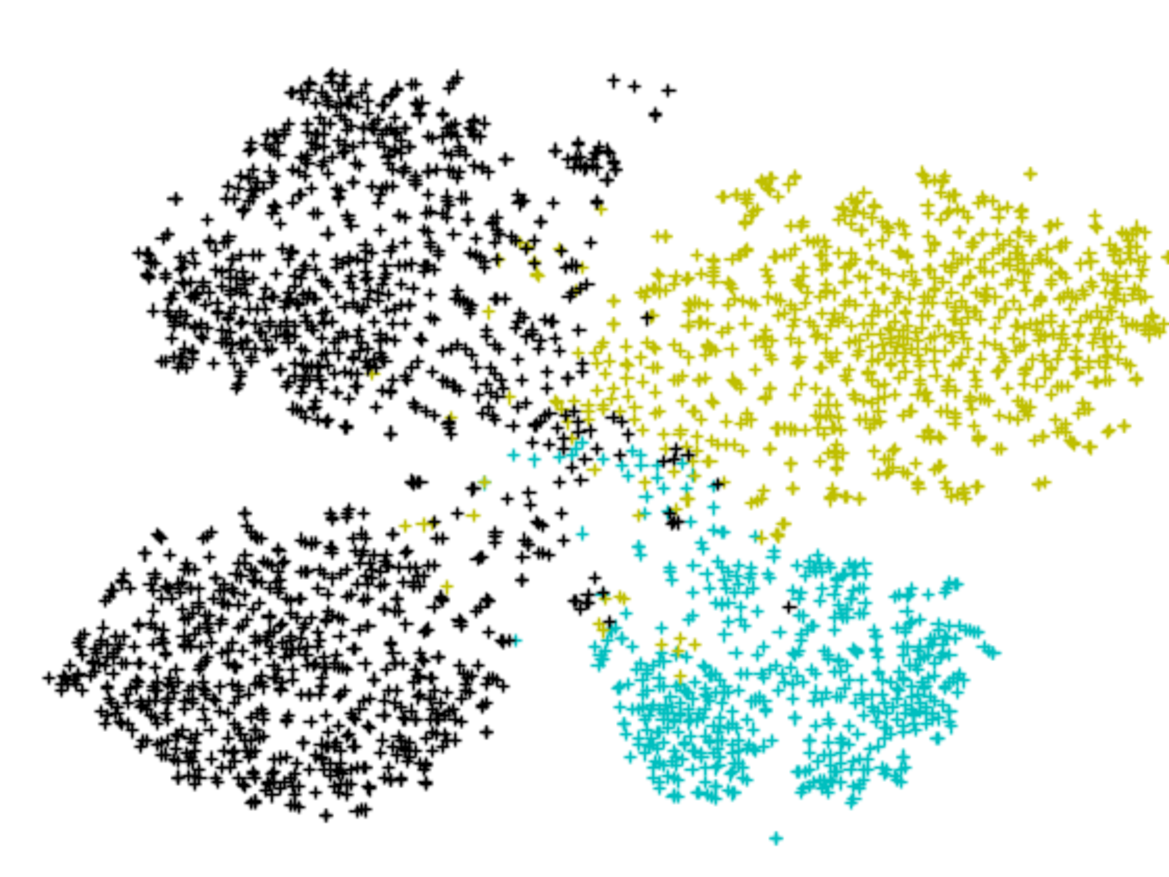
\includegraphics[width=\linewidth]{images/none}
    \caption{}
    \label{fig:null}
  \end{subfigure}
%
  \begin{subfigure}[b]{0.38\linewidth}
    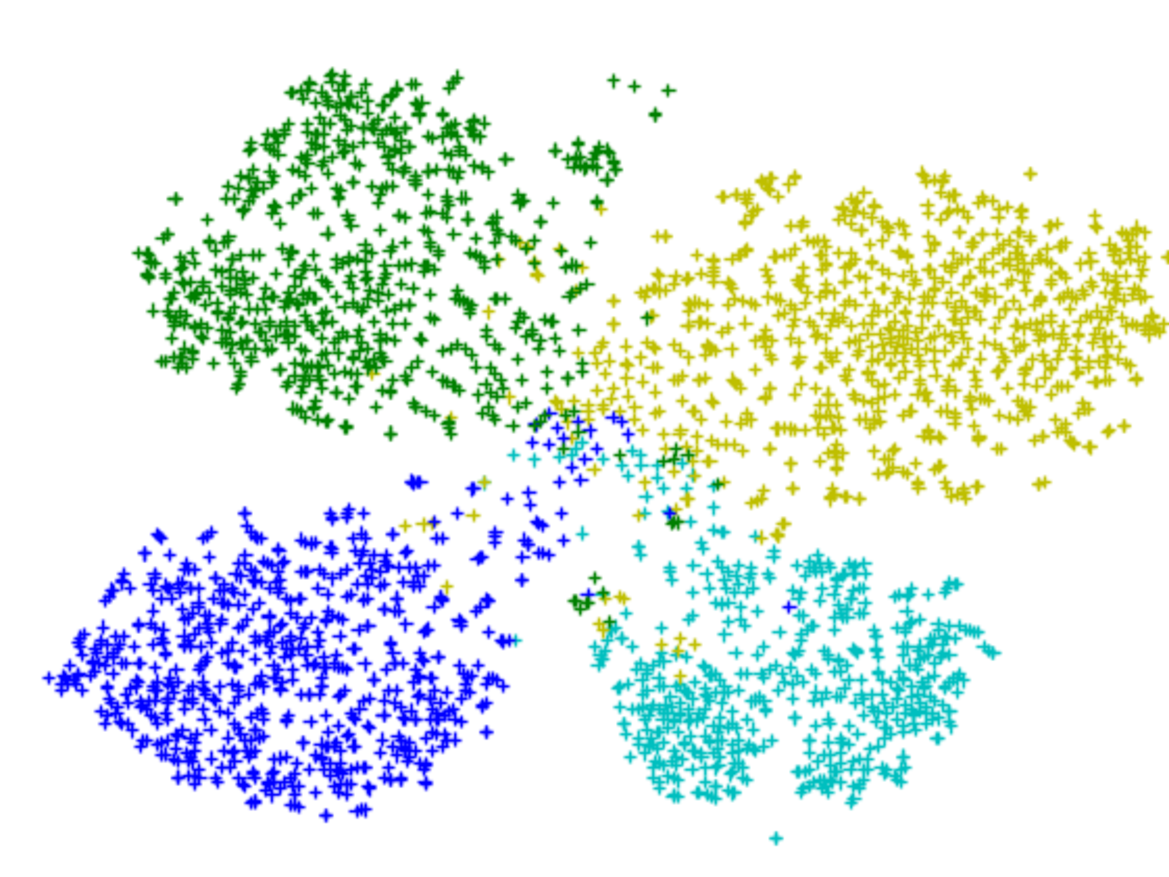
\includegraphics[width=\linewidth]{images/truth}
    \caption{}
% \caption{Points colored according to their ground truth labels}
    \label{fig:truth}
  \end{subfigure}
%
  \begin{subfigure}[b]{0.38\linewidth}
    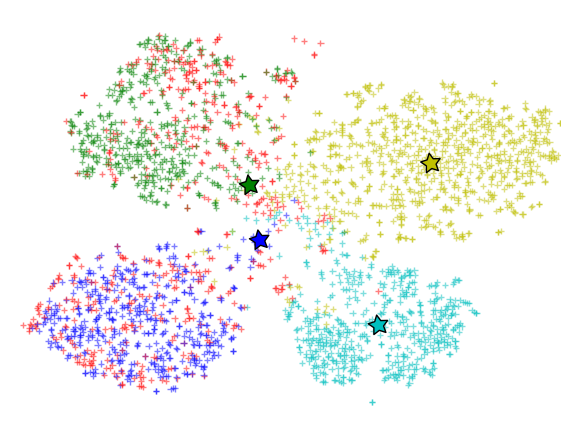
\includegraphics[width=\linewidth]{images/knn}
    % \caption{Signatures mapped to image spacing using Eq. \eqref{eq:dic} and denoted by stars. Then classification done using nearest neighbor}
    \caption{}
\label{fig:knn}
  \end{subfigure}
%
  \begin{subfigure}[b]{0.38\linewidth}
    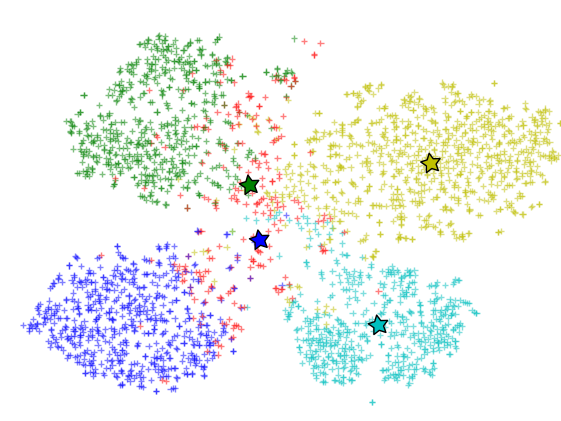
\includegraphics[width=\linewidth]{images/kmeans}
    % \caption{Stars as previous. Classification done by our compatibility function on cluster assignments from k-means}
    \caption{}
\label{fig:kmeans}
  \end{subfigure}
%
  \begin{subfigure}[b]{0.38\linewidth}
    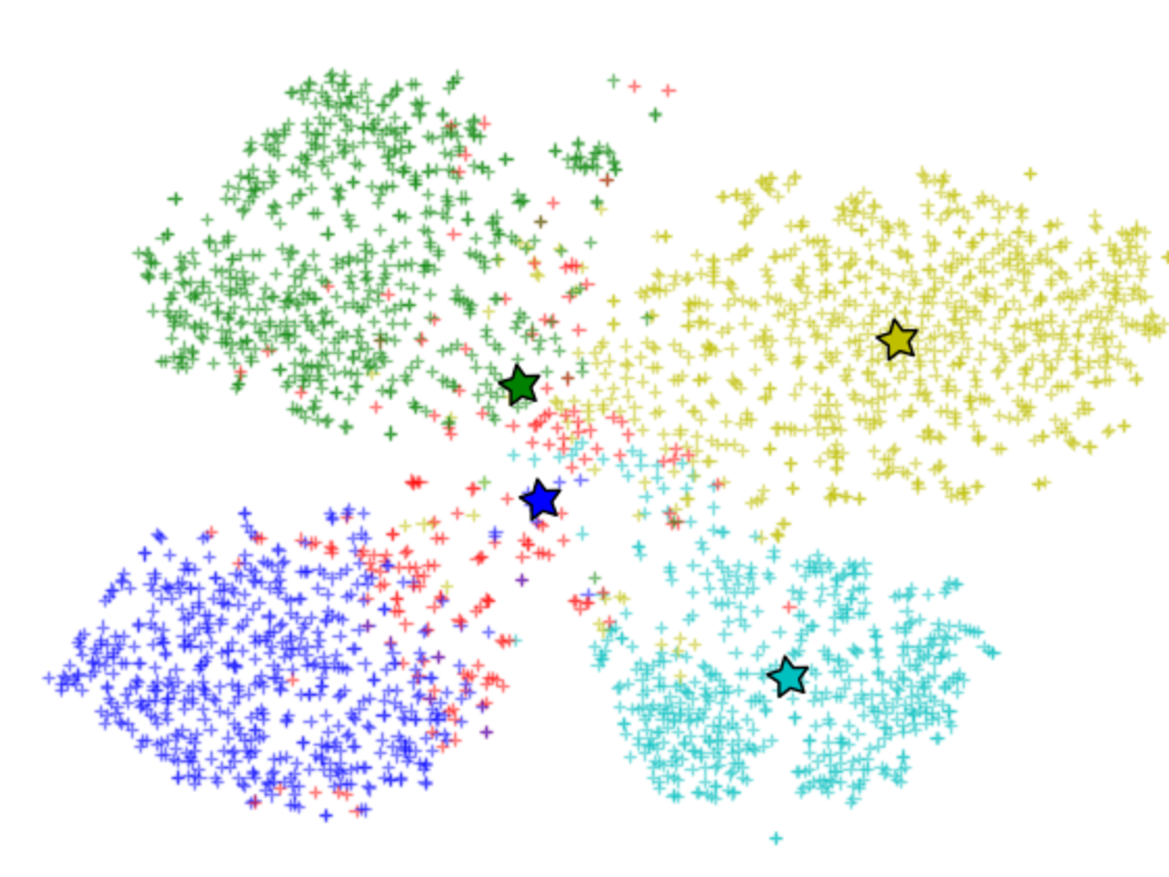
\includegraphics[width=\linewidth]{images/own_cluster}
    \caption{}
    \label{fig:clustering}
% \caption{Stars as previous. Classification by our compatibility function using our supervised clustering}
  \end{subfigure}
%
  \begin{subfigure}[b]{0.38\linewidth}
    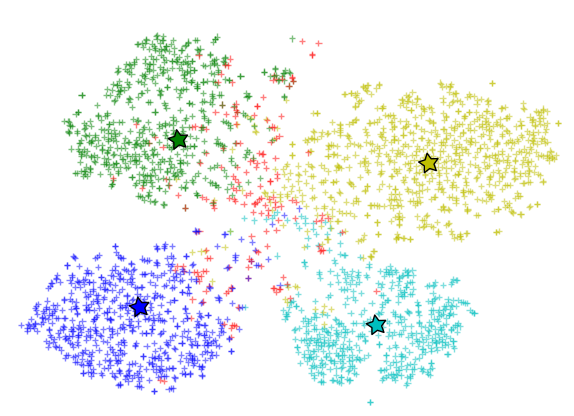
\includegraphics[width=\linewidth]{images/jeac}
    \caption{}
    \label{fig:jeac}
% \caption{Class signatures mapped to image space (stars) and cluster assignment by JEaC}
  \end{subfigure}
  \caption[تحلیل قسمت‌های مختلف روش پیشنهادی]{
  نمایش دوبعدی چهار دسته از مجموعه دادگان AwA با استفاده از نگاشت \lr{t-SNE}، دو دسته‌ی دیده شده شامل بزگوزن (فیروزه‌ای) خرس گریزلی (زرد) و دو دسته‌ی دیده نشده شامپانزه (آبی) و پاندا (سبز). تصاویر با نماد بعلاوه و نگاشت توصیف دسته‌ها در فضای تصاویر با ستاره نشان داده شده است. در تصاویر (ب) تا (و) نقطه‌های قرمز نمونه‌هایی که را نشان می‌دهد که دسته‌ای به جز چهار دسته‌ی موجود در شکل برای آن‌ها پیش‌بینی شده است.
  \textbf{آ)}
   دسته‌های دیده شده با برچسب صحیح و دیده‌نشده با رنگ مشکی
\textbf{ب)}
 نمایش برچسب صحیح برای تمامی دسته‌ها
  \textbf{ج)} توصیف‌ها با نگاشت \eqref{eq:d_answer}
  به فضای تصاویر برده شده‌اند و دسته‌بندی با دسته‌بند نزدیک‌ترین همسایه انجام شده است.
  \textbf{د)}
   نگاشت مانند حالت قبل و دسته‌بندی با تابع مطابقت پیشنهادی به همراه خوشه‌بند \lr{k-means}
  \textbf{هـ)}
   نگاشت مانند حالت قبل و دسته‌بندی با تابع مطابقت پیشنهادی به همراه خوشه‌بند نیمه‌نظارتی پیشنهاد شده
  \textbf{و)}
  دسته‌بندی و نگاشت با استفاده از روش پیشنهادی برای یادگیری نگاشت و خوشه‌بندی توام.
  }
\label{fig:discussion}
\end{figure}

\section{جمع‌بندی}\label{exp:conclusion}
در این فصل نتایج آزمایشات عملی برای روش‌های مختلف پیشنهادی در فصل قبل ارائه شد. ابتدا در بخش \ref{exp:datasets} مجموعه‌دادگان مورد استفاده معرفی شدند. در ادامه
در بخش \ref{exp:nn} شبکه عصبی چندوظیفه‌ای پیشنهادی مورد بررسی قرار داده شد و نتایج آن با سایر روش‌های پیش‌بینی صفت و هم‌چنین حالت ساده شده که از نمونه‌های آزمون استفاده نمی‌کند مقایسه شد. همچنین در بخش \ref{exp:nn_comp} تابع مطابقت پیشنهادی به خروجی این شبکه اضافه شد که دقت پیش‌بینی‌های انجام شده را افزایش داد. در بخش \ref{exp:cluster} عمل‌کرد روش خوشه‌بندی نیمه‌نظارتی پیشنهادی مورد بررسی قرار گرفت. در بخش  \ref{exp:simple}  روش دسته‌بندی با نگاشت به فضای تصاویر و استفاده از تابع مطابقت پیشنهادی و خوشه‌‌بندی نیمه‌نظارتی مورد آزمایش قرار گرفت و در بخش نتایج مربوط \ref{exp:jeac} روش یادگیری و خوشه‌بندی توام ارائه شد. در نهایت در بخش \ref{exp:discussion} نتایج مورد بررسی و مقایسه قرار گرفتند و علل عمل‌کرد برتر روش‌های پیشنهادی عنوان شد.

\chapter{جمع‌بندی} \label{chap:conclusion}
\section{جمع‌بندی}
در این پژوهش مسئله یادگیری بدون برد را برای دسته‌بندی تصاویر مورد بررسی قرار دادیم. در این مسئله برای برخی دسته‌ها در زمان آموزش نمونه‌ی برچسب‌داری در اختیار نیست و این دسته‌ها با استفاده از یک نوع اطلاعات جانبی مشخص می‌شوند و برای آن‌ها دسته‌بند ساخته می‌شود. ابتدا یک چهارچوب کلی برای روش‌های موجود در مسئله یادگیری بدون برد ارائه کردیم. این چهارچوب شامل سه گام ۱) نگاشت تصاویر به یک فضای میانی، ۲) نگاشت توصیف‌ها به فضای میانی و ۳) دسته‌بندی در فضای میانی بود. سپس روش‌های پیشین در قالب این چهارچوب مرور شدند. در این مرور مشاهده کردیم که به استفاده از اطلاعات بدون نظارت موجود در ساختار فضای تصاویر کمتر توجه شده است. 

در ادامه برای استفاده از اطلاعات موجود در ساختار فضای تصاویر، یک تابع مطابقت مبتنی بر خوشه‌بندی تصاویر بیان کردیم که قابلیت اضافه شدن به روش‌های پیشین و بهبود آن‌ها را داراست. با توجه به تکیه‌ی این تابع مطابقت به یک خوشه‌بندی از تصاویر یک روش خوشه‌بندی نیمه‌نظارتی ارائه دادیم که با ساختار و فرض‌های مسئله یادگیری بدون برد منطبق باشد. دو معماری شبکه عصبی ژرف برای نگاشت تصاویر به بردارهای صفت و یا هیستوگرامی از دسته‌های دیده شده ارائه شد و از آن‌ها به همراه تابع مطابقت پیشنهادی برای دسته‌بندی بدون نمود نمونه‌ای استفاده شد. هم‌چنین با ترکیب تابع مطابقت و خوشه‌بندی نیمه‌نظارتی معرفی شده،  روشی برای مسئله یادگیری بدون برد تحت عنوان خوشه‌بندی و یادگیری نگاشت مجزا پیشنهاد کردیم که به نتایجی بهتر از نتایج پیشگام روش‌های پیشین در اکثر آزمایشات دست پیدا کرد. برای رفع نقایص این روش و  افزایش بیشتر دقت دسته‌بندی، روش پیشنهادی دیگری را تحت عنوان یادگیری نگاشت و خوشه‌بندی توام ارائه کردیم که محدودیت‌های ناشی از جدا بودن این مراحل در روش قبلی را برطرف کرده و دقت دسته‌بندی را افزایش داد. 
\section{کار‌های آینده}
با توجه به این مسئله که روش‌هایی که برای توصیف دسته‌های دیده نشده از هیستوگرام شباهت به دسته‌های دیده شده استفاده می‌کنند، به رغم این‌که از اطلاعات نمونه‌های آزمون استفاده نمی‌کنند، نتایج نزدیکی به روش نیمه‌نظارتی پیشنهاد شده توسط ما نزدیک است، بنظر می‌رسد یک شاخه امیدوارکننده برای ادامه پژوهش ترکیب این دو رویکرد باشد. یعنی نگاشت تصاویر و توصیف‌ها به فضای هیستوگرامی از دسته‌های دیده شده به صورتی که یادگیری این نگاشت‌ها و/یا دسته‌بندی در آن فضای مشترک با توجه و استفاده از نمونه‌های آزمون باشد.

یک شاخه دیگر که برای ادامه می‌تواند در نظر گرفته باشد ترکیب رویکرد شبکه‌های عصبی با روش‌های دیگر ارائه شده است، در این حالت با ویژگی‌های تصویر بکارگرفته شده در روش‌های ارائه شده در بخش‌های
\ref{simple_method}
و \ref{jeac}، به جای این که ثابت فرض شوند می‌توانند در جریان آموزش همراه با سایر پارامترها تعیین شوند.

استفاده از اطلاعات جانبی دیگر مانند نمایش برداری نام دسته‌ها به عنوان یک شاخه دیگر مطرح است که با توجه به ضعیف‌تر بودن اطلاعات نظارتی موجود در این نوع امضای  دسته‌ها نسبت به بردار توصیف استفاده شده در این پژوهش، اطلاعات بدون نظارت موجود در نمونه‌های بدون برچسب  می‌تواند موثرتر باشند و بهبود بیشتری ایجاد کند.

پیش‌بینی صفت‌های موجود درون تصویر با استفاده از شبکه‌های عصبی \gls{recurrent} یک ایده‌ی قابل پیگیری دیگر است. با توجه به این که این شبکه‌ها امکان مدل‌سازی روابط صفات را دارا هستند، پیش‌بینی ویژگی با استفاده از این شبکه‌ها می‌تواند نتایج بهتری نسبت به مدل‌هایی که صفات را مستقل فرض می‌کنند داشته باشد. 

%\include{chapters/6}


% -------------------- Bibliography --------------------

\renewcommand{\bibname}{\rl{کتاب‌نامه} }

% -------------------------------------------------------
%  Bibliography
% -------------------------------------------------------


\begin{latin}
\baselineskip=.8\baselineskip


% Uncomment next line to include uncited references
\nocite{*}

\bibliography{bibs/references}
\bibliographystyle{./packages/unsrtabbrv}

\end{latin}
\newpage

\printglossary
%\printabbreviation \newpage
% -------------------- Back Pages --------------------
\newgeometry{left=3cm,right=2.5cm}

% -------------------------------------------------------
%  English Abstract
% -------------------------------------------------------


\pagestyle{empty}
\begin{latin}
  \textbf{Abstract}
In some of object recognition problems, labeled data may not be available for all categories.
 Zero-shot learning utilizes auxiliary information (also called signatures)
 describing each category in order to find a classifier that can recognize samples
from categories with no labeled instance. %RR It is usually only unseen classes
On the other hand, with recent advances made by deep neural networks in computer vision, a rich representation can be obtained from images
that discriminates different categorizes and therefore a obtaining unsupervised information from images is made possible.
However in the previous works, little attention has been paid to using such unsupervised information for task of zero-shot learning.
In this work, we first propose a multi-task neural network to predict attributes from images while exploiting this unsupervised information
in order to mitigate the so called \textit{domain shift problem} in predictions on unseen data.
We also propose a novel semi-supervised zero-shot learning method that works on an embedding space corresponding to
abstract deep visual features. We seek a linear transformation on signatures to map them onto the visual features,
such that the mapped signatures of the seen classes are close to labeled samples of the corresponding
classes and unlabeled data are also close to the mapped signatures of one of the unseen classes.
 We use the idea that the rich deep visual features provide a representation
 space in which samples of each class are usually condensed in a cluster. The effectiveness of the proposed method is demonstrated through extensive
experiments on four public benchmarks improving the state-of-the-art prediction accuracy on three of them.

\bigskip\noindent\textbf{Keywords}:
Zero-shot Learning, Semi-supervised Learining, Deep Learning, Representation Learning.
\end{latin}

\newpage

%-@@@@@@@@@@@@@@@@@@@@@@2-Uncmment:@@@@@@@@@@@@@@@@@@@@@

% -------------------------------------------------------
%  English Thesis Information
% -------------------------------------------------------


\def \MyThesisEnglish {
M.Sc. Thesis \\
Artificial Intelligence
}

\def \MyThesisTitleEnglish {Deep Zero-shot Learning}

\def \MyNameEnglish {
Seyed Mohsen Shojaee
}

\def \MyProfessorEnglish {
Dr. Mahdaieh Soleymani
}

\def \MyPresentationDateEnglish {
Summer 2017
}


\def \MyUniversityEnglish {
Sharif University of Technology
}

\def \MyDepartmentEnglish {
Department of Computer Engineering
}



\pagestyle{empty}

\begin{center}

\begin{latin}

\vspace{0.2cm}


\includegraphics[scale=0.2]{front/template/images/logo.png}

\begin{large}

\MyUniversityEnglish

\MyDepartmentEnglish

\vspace{0.5cm}
\Large\MyThesisEnglish

\end{large}

\vspace{1.3cm}

\LARGE{\textbf{\MyThesisTitleEnglish}}\\

\vspace{1.5cm}

\large{By:}\\
\Large{\textbf{\MyNameEnglish}}\\

\vspace{1cm}

\large{Supervisor:}\\ 
\vspace{0.0cm}
\Large{\textbf{\MyProfessorEnglish}}\\

\vspace{1.3cm}

\large{\MyPresentationDateEnglish}

\end{latin}

\end{center}

\newpage



% -------------------- The End! --------------------

\end{document}
